\documentclass[acmlarge, preprint, authorversion]{acmart}
\settopmatter{printacmref=false}

\pagestyle{plain}
\usepackage{hyperref}

\hypersetup{colorlinks=true,allcolors=blue}

\hypersetup{
    colorlinks=true,
    linkcolor=blue,
    urlcolor=blue,
    citecolor=blue
}

% \usepackage{tipa}
% \usepackage{inconsolata}
\usepackage{amsmath,amssymb,latexsym}
\usepackage{amsmath}
\usepackage{amsthm}
\usepackage{comment}
%\usepackage{amsfonts}
%\usepackage{amssymb}
%\usepackage{mathtools}
\usepackage{commands}
\usepackage{liquidHaskell}
\usepackage{xspace}
\usepackage{epsfig}
\usepackage{booktabs}
\usepackage{listings}
% \usepackage{stmaryrd}
\usepackage{flushend}
\usepackage{ifthen}
\usepackage[outdir=./]{epstopdf}

% \bibliographystyle{ACM-Reference-Format}
% \citestyle{acmauthoryear}

% \renewcommand{\ttdefault}{pcr}

% \newtheorem{theorem}{Theorem}
% \newtheorem{lemma}{Lemma}
% \newtheorem{definition}{Definition}
% \newtheorem{corollary}{Corollary}

\usepackage{thmtools}
\declaretheoremstyle[%
  spaceabove=-6pt,%
  spacebelow=6pt,%
  headfont=\normalfont\itshape,%
  postheadspace=1em,%
  qed=\qedsymbol,%
  headpunct={}
]{mystyle}
\declaretheorem[name={Proof:},style=mystyle,unnumbered,
]{myproof}

\usepackage[inference]{semantic}

\usepackage{listings}
\usepackage{amssymb}

% uncomment next line to restore colors
\def\withcolor{}


\ifdefined\withcolor
	 \definecolor{haskellblue}{rgb}{0.0, 0.0, 1.0}
	 \definecolor{haskellstr}{rgb}{0.2, 0.2, 0.6}
	 \definecolor{haskellred}{rgb}{1.0, 0.0, 0.0}
     \definecolor{gray_ulisses}{gray}{0.55}
     \definecolor{castanho_ulisses}{rgb}{0.71,0.33,0.14}
     \definecolor{preto_ulisses}{rgb}{0.41,0.20,0.04}
     \definecolor{green_ulises}{rgb}{0.2,0.75,0}
     \definecolor{haskelltypes}{rgb}{0.71,0.33,0.14}
     \definecolor{logiccolor}{rgb}{0.0, 0.0, 1.0}
\else
	\definecolor{haskellblue}{gray}{0.1}
	\definecolor{haskellstr}{gray}{0.1}
	\definecolor{haskellred}{gray}{0.1}
	\definecolor{gray_ulisses}{gray}{0.1}
	\definecolor{castanho_ulisses}{gray}{0.1}
	\definecolor{preto_ulisses}{gray}{0.1}
	\definecolor{green_ulisses}{gray}{0.1}
	\definecolor{haskelltypes}{gray}{0.1}
    \definecolor{logiccolor}{gray}{0,1}
\fi

% RJ: I don't like the colors. Too confusing.
%
% \definecolor{lcolor}{rgb}{0.0, 0.0, 1.0}
% \definecolor{lappcolor}{rgb}{1.0, 0.0, 0.0}
% \definecolor{lappascolor}{rgb}{0.0, 1.0, 0.0}

\definecolor{lcolor}{gray}{0.0}
\definecolor{lappcolor}{gray}{0.0}
\definecolor{lappascolor}{gray}{0.0}

\def\codesize{\small}
% \def\codesize{\footnotesize}

% \newcommand\showfocus[1]{\color{lappcolor}{#1}}
% \newcommand\showfocus[1]{\underbar{#1}}
\newcommand\showfocus[1]{\color{purple}{\textbf{#1}}}
\newcommand\showlogic[1]{\color{logiccolor}{#1}}

\lstdefinelanguage{HaskellUlisses} {
	basicstyle=\ttfamily\codesize,
	moredelim=[is][\showfocus]{\#}{\#},
	moredelim=[is][\showlogic]{!}{!},
	sensitive=true,
	morecomment=[l][\color{gray_ulisses}\ttfamily\itshape\codesize]{--},
	morecomment=[s][\color{gray_ulisses}\ttfamily\itshape\codesize]{\{-}{-\}},
	morestring=[b]",
    %% escapeinside={(*}{*)},
	stringstyle=\color{haskellstr},
	showstringspaces=false,
	numberstyle=\codesize,
	numberblanklines=true,
	showspaces=false,
	breaklines=true,
	showtabs=false,
  %% whitespace hackery
  %% lineskip=-2pt,
  %% % aboveskip=\smallskipamount,
  %% belowskip=0pt,
  literate={
	         {<!}{{{\color{lcolor}<!}}}2
           {==!}{{{\color{lcolor}==!}}}3
           {`}{{{$^{\backprime}{}$}}}1
           % {QED}{{{\color{lcolor}QED}}}3
           % {***}{{{\color{lcolor}***}}}3
           {?}{{{\color{lcolor}?}}}1
           {<=}{{$\leq$}}1
           {theta}{{$\theta$}}1
           {rf}{{{\color{lappcolor}f}}}1
           {gf}{{{\color{lappascolor}f}}}1
           {rmap}{{{\color{lappcolor}map}}}3
           {gmap}{{{\color{lappascolor}map}}}3
           {r.}{{{\color{lappcolor}.}}}1
           {g.}{{{\color{lappascolor}.}}}1
           {r++}{{{\showfocus{++}}}}2
           {g++}{{{\color{lappascolor}++}}}2
           %{r>>=}{{{\color{lappcolor}>>=}}}3
           %{g>>=}{{{\color{lappascolor}>>=}}}3
           {gfib}{{{\color{lappascolor}fib}}}3
           {rfib}{{{\color{lappcolor}fib}}}3
           {r++}{{{\color{lappcolor}++}}}2
           % {>>=}{$\ebind$}2
           {op}{{$\odot$}}1
           {env}{{$\Gamma$}}1
           {|-}{{$\vdash$}}1
          % {>=}{{$\geq$}}1
          % {<}{{$<$}}1
          % {>}{{$>$}}1
           {<=!}{{{\color{lcolor}<=!}}}3
          % {\\}{{$\lambda$}}1
           {!=}{{$\neq$}}1
           {forall}{{$\forall$}}1
           {->}{{$\rightarrow$}}2
           {=*}{{$\eqfun$}}2
           {Set_mem}{{$\in$}}1
           {Set_cup}{{$\cup$}}1
           {Set_cap}{{$\cap$}}1
           {Set_emp}{{$\emptyset$}}1
           {Set_sub}{{$\subseteq$}}1
           {<=>}{{$\Leftrightarrow$}}3
           {=>}{{$\Rightarrow$}}2
           {1->}{{$\rightarrow$}}1
           {1=>}{{$\Rightarrow$}}1
           {||-}{{$\vdash$}}1
           {|->}{{$\mapsto$}}2
           {<:}{{$\preceq$}}1
           {Inarritu}{Inarritu}8},
%           {Inarritu}{I$\tilde{\text{n}}\acute{\text{a}}$rritu}8,
	emph=
	{[1]
		FilePath,IOError,abs,acos,acosh,all,and,any,appendFile,approxRational,asTypeOf,asin,
		asinh,atan,atan2,atanh,basicIORun,break,catch,ceiling,chr,compare,concat,concatMap,
		cos,cosh,curry,cycle,decodeFloat,denominator,digitToInt,div,divMod,drop,
		dropWhile,either,elem,encodeFloat,enumFrom,enumFromThen,enumFromThenTo,enumFromTo,
		error,even,exponent,fail,mapMaybe,filter,flip,floatDigits,floatRadix,floatRange,floor,
		foldl,foldl1,foldr1,fromDouble,fromEnum,fromInt,fromInteger,fromIntegral,
		fromRational,fst,gcd,getChar,getContents,getLine,head,inRange,index,init,intToDigit,
		interact,ioError,isAlpha,isAlphaNum,isAscii,isControl,isDenormalized,isDigit,isHexDigit,
		isIEEE,isInfinite,isLower,isNaN,isNegativeZero,isOctDigit,isPrint,isSpace,isUpper,iterate,
		last,lcm,length,lex,lexDigits,lexLitChar,lines,log,logBase,lookup,mapM,mapM_,max,
		maxBound,posMax,negMax,maximum,maybe,min,minBound,minimum,mod,negate,notElem,null,numerator,odd,
		or,ord,pi,pred,primExitWith,print,product,putChar,putStr,putStrLn,quot,
		quotRem,range,rangeSize,read,readDec,readFile,readFloat,readHex,readIO,readInt,readList,readLitChar,
		readLn,readOct,readParen,readSigned,reads,readsPrec,realToFrac,recip,rem,repeat,replicate,return,
		reverse,round,scaleFloat,scanl,scanl1,scanr,scanr1,seq,sequence,sequence_,show,showChar,showInt,
		showList,showLitChar,showParen,showSigned,showString,shows,showsPrec,significand,signum,sin,
		sinh,snd,span,splitAt,sqrt,subtract,succ,tail,take,takeWhile,tan,tanh,threadToIOResult,toEnum,
		toInteger,toLower,toRational,toUpper,truncate,uncurry,undefined,unlines,until,unwords,unzip,
		unzip3,userError,words,writeFile,zip,zip3,zipWith,zipWith3,listArray,doParse,empty,for,initTo,
        assert,compose,checkGE,maxEvens,empty,create,get,set,initialize,idVec,fastFib,fibMemo,
        ex1,ex2,ex3,incr,inc,dec,isPos,positives,find,len,size,union,fromList,initUpto,trim,
        insertSort,decsort,qsort,reverse,append,upperCase, ifM, whileM, get, decrM, diff,
        project, select, elts, keys, dkeys, dfun, addKey, pTrue, emptyRD, rFalse,
        	dom, rng, isI, isD, isS, movie1, movie2,  toI, toS, toD, good_titles, runState, ret,
        	update, getCtr, setCtr, ctr, rdCtr, wrCtr, ifTest, whileTest, posCtr, zeroCtr, decr, decCtr,
        	pread , pwrite , plookup , pcontents, pcreateF , pcreateFP, pcreateD, active, caps, pset, eqP,
        	write, contents, alloc, derivP, copyP, createDir, store, copyRec, copySpec,
        	forM_, when, flookup, fread, createDir, pcreateFile, isFile, copyFrame, ?
	},
	emphstyle={[1]\color{haskellblue}},
	emph=
	{[2]Show,Eq,Iso,VerifiedOrd,Ord,Num,UpClosed,Comp,Wit,Witness,Inductive,Meet,Flip,TRUE,
	    Peano,Nat,Pos,Neg,IntGE,Plus,List,
        Bool,Char,Double,Either,Float,IO,Integer,Int,Maybe,
        Ordering,Rational,Ratio,ReadS,ShowS,String,Word8,
        InPacket,Tree,Vec,NullTerm,IncrList,DecrList,
        UniqList,BST,MinHeap,MaxHeap,World,RIO,IO,HIO,Post,Pre,
        Privilege, Prop, Chain, ChainTy, Range, Dict, RD, Dom, Set, P, Univ, Schema, MovieSchema, RT,
        TDom, TRange, MoviesTable, RTSubEqFlds, RTEqFlds, Disjoint, Union, Ret, Seq, Trans, Map,
        Pure, Then, Else, Exit, Inv, OneState, Priv, Path, FH, Stable,
	    Nat, Monoid, VerifiedMonoid, VerifiedComMonoid, Plus_2_2_eq_4, Plus_com, Par, Term,
	    Formula, Assignment, Body, Accel, Real, Accel', RVar, VerifiedCommutativeMonoid
	},
	emphstyle={[2]\color{castanho_ulisses}},
	emph=
	{[3]
		case,class,newtype,data,deriving,do,else,if,import,in,infixl,infixr,instance,let,
		module,of,primitive,then,refinement,type,where,forall,bound,
		% otherwise,
		measure,reflect,predicate
	},
	emphstyle={[3]\color{preto_ulisses}\textbf},
	emph=
	{[4]
		quot,rem,div,mod,elem,notElem,seq
	},
	emphstyle={[4]\color{castanho_ulisses}\textbf},
	emph=
	{[5]
		EQ,GT,LT,Left,Right
		%, False, True, Just, Nothing
	},
	emphstyle={[5]\color{preto_ulisses}\textbf},
	emph=
	{[6]
	    axiomatize, measure, inline
	},
	emphstyle={[6]\color{lcolor}}
}

%%%ORIG
%%%\lstnewenvironment{code}
%%%{\textbf{Haskell Code} \hspace{1cm} \hrulefill \lstset{language=HaskellUlisses}}
%%%{\hrule\smallskip}

%V1
%\lstnewenvironment{code}
%{\smallskip \lstset{language=HaskellUlisses}}
%{\smallskip}

\lstnewenvironment{code}
{\lstset{language=HaskellUlisses}}
{}

\lstnewenvironment{mcode}
{\lstset{language=HaskellUlisses,columns=fullflexible,keepspaces,mathescape}}
{}

\lstMakeShortInline[language=HaskellUlisses,mathescape,keepspaces,mathescape,basicstyle=\ttfamily\normalsize,breakatwhitespace]@


\lstdefinelanguage{Pseudo} {
	basicstyle=\ttfamily\codesize,
	sensitive=true,
  mathescape=true,
	morecomment=[l][\color{gray_ulisses}\ttfamily\codesize]{--},
	morecomment=[s][\color{gray_ulisses}\ttfamily\codesize]{\{-}{-\}},
	morestring=[b]",
	showstringspaces=false,
	numberstyle=\codesize,
	numberblanklines=true,
	showspaces=false,
	breaklines=true,
	showtabs=false
}

\lstdefinelanguage{java} {
    keywordstyle=[1],
    keywordstyle=[2]\color{ForestGreen},
    keywordstyle=[3]\color{Bittersweet},
    keywordstyle=[4]\color{RoyalPurple},
    morekeywords={region,private,synchronized}
}


\newcommand{\isTechReport}{false} % true or false
\acmYear{2017}
\acmMonth{2}

\begin{document}


%\title{From Types to Proofs via Refinement Reflection}
%\title{\ifthenelse{\equal{\isTechReport}{true}}
%       {{Technical Report:}}
%        {}
%        Refinement Reflection
%       }
%\subtitle{\emph{(or, how to convert a legacy programming language into a proof assistant)\vspace{-17mm}}}

\ifthenelse{\equal{\isTechReport}{true}}{
\title{Technical Report: Refinement Reflection:}
}{
\title{Refinement Reflection:}
}
% \authorinfo{}{}
% \authorinfo{OMITTED FOR BLIND REVIEW}{}
% \authorinfo{Niki Vazou \and Ranjit Jhala}{University of California, San Diego}{}

\subtitle{Parallel Legacy Languages as Theorem Provers}


\begin{abstract}
We introduce \emph{refinement reflection}, a method
to extend \emph{legacy} languages---with highly tuned
libraries, compilers, and run-times---into theorem provers.
%
The key idea is to reflect the code implementing a
user-defined function into the function's (output)
refinement type.
%
As a consequence, at \emph{uses} of the function,
the function definition is unfolded into the refinement logic
in a precise and predictable manner.
%
We have implemented our approach in \toolname
thereby retrofitting theorem proving into Haskell.
%
We show how to use reflection to verify
that many widely used instances of the Monoid,
Applicative, Functor, and Monad typeclasses
actually satisfy key algebraic laws required to 
make the code using the typeclasses safe.
%
Finally, transforming a mature language---with
highly tuned parallel runtime---into a theorem
prover  enables us to build the first
\emph{deterministic parallelism library}
that verifies assumptions about associativity
and ordering---that are crucial for determinism
but simply assumed by existing systems.
\end{abstract}

% \vspace{-5mm}

%%\begin{abstract}
%%Refinement Reflection turns your favorite programming
%%language into a proof assistant by reflecting
%%the ​code implementing a​ user-defined function
%%into the function's (output) refinement type.
%%%
%%As a consequence, at \emph{uses} of the function,
%%the function definition is unfolded into the refinement logic
%%in a precise, predictable and most
%%importantly, programmer controllable way.
%%%
%%In the logic, we encode functions and lambdas using uninterpreted symbols
%%preserving SMT-based decidable verification.
%%In the language, we provide a library of combinators that lets programmers
%%compose proofs from basic refinements and function definitions.
%%%
%%We have implemented our approach in the Liquid Haskell system,
%%thereby converting Haskell into an interactive proof assistant,
%%that we used to verify a variety of properties ranging
%%from arithmetic properties of higher order, recursive functions
%%to the Monoid, Applicative, Functor and Monad type class laws
%%for a variety of instances.
%%%
%%\new{Finally, transforming a mature language---with a parallel runtime---into a proof
  %%assistant enables us to build the first {\em deterministic parallelism
    %%library} that verifies assumptions about associativity and
  %%ordering---necessary to determinism but simply assumed by existing systems.}
%%\end{abstract}



%% Author with two affiliations and emails.
\author{Niki Vazou}
\affiliation{
  \institution{University of Maryland}           %% \institution is required
}


\author{Ranjit Jhala}
\affiliation{
  \institution{UC San Diego}           %% \institution is required
}

\author{Vikraman Choudhury}
\author{Ryan Scott}
\author{Ryan Newton}
\affiliation{
  \institution{Indiana University}            %% \institution is required
}
% \email{first1.last1@inst1.edu}          %% \email is recommended


\maketitle

\section{Introduction}\label{sec:intro}

We introduce \emph{refinement reflection}, a method
to extend \emph{legacy} programming languages---with highly tuned
libraries, compilers, and run-times---into theorem provers,
by letting programmers specify and verify
arbitrary properties of their code simply
by writing programs in the legacy language.

Previously, SMT-based refinement types
\citep{ConstableS87,Rushby98} have been
used to retrofit so-called ``shallow''
verification \eg array bounds checking into
%
ML~\cite{pfenningxi98,GordonRefinement09,LiquidPLDI08},
%
C~\cite{deputy,LiquidPOPL10},
%
Haskell~\citep{Vazou14},
%
TypeScript~\cite{Vekris16}, and
%
Racket~\cite{RefinedRacket}.
%
% Scala~\cite{ScalaLiquidTyper}.
%
To keep checking decidable, the specifications
are restricted to quantifier free formulas over
decidable theories.
%
However, to verify ``deep'' specifications as
in theorem proving languages like Agda, Coq, Dafny,
\fstar and Idris we require mechanisms that
\emph{represent} and \emph{manipulate} the
exact descriptions of user-defined functions.
%
So far, this has entailed either building new
languages on specialized type theories or
encoding functions with SMT axioms which makes
verification undecidable and hence, unpredictable.

% Refinement reflection lets us retrofit
% theorem proving onto legacy languages,
% while keeping verification decidable
% and predictable.
%
\mypara{1. Refinement Reflection}
%
Our first contribution is the notion of
refinement reflection: the code
implementing a user-defined function can
be \emph{reflected} into the function's
(output) refinement type, thus converting
the function's (refinement) type signature
into a deep specification of the functions
behavior.
%
This simple idea has a profound consequence:
at \emph{uses} of the function, the standard
rule for (dependent) function application
yields a precise, predictable and most
importantly, programmer controllable
means of \emph{instantiating} the deep
specification that is not tethered to
brittle SMT heuristics.
%
Specifically, we show how to use ideas for
\emph{defunctionalization} from the theorem
proving literature which encode functions
and lambdas using uninterpreted symbols,
to encode terms from an expressive higher
order language as decidable refinements,
letting us use SMT-based congruence
closure for decidable and predictable
verification~(\S~\ref{sec:theory}).

\mypara{2. A Library of Proof Combinators}
%
Our second contribution is a
\emph{library of combinators}
that lets programmers
\emph{compose proofs}
from basic refinements
and function definitions.
%
We show how to represent proofs
simply as unit-values refined
by the proposition that
they prove. %~(\S~\ref{sec:library}).
%
We show how to build up sophisticated proofs
using a small library of combinators that
permits reasoning in an algebraic or
equational style.
%
Furthermore, since proofs are literally
just programs, our proof combinators let
us use standard language mechanisms like
branches (to encode case splits),
recursion (to encode induction), and
functions (to encode auxiliary lemmas)
to write proofs that look very much like
transcriptions of their pencil-and-paper
analogues~(\S~\ref{sec:overview}).

\mypara{3. Verified Typeclass Laws}
%
Our third contribution is an implementation
of refinement reflection in \toolname~\citep{Vazou14},
thereby converting the legacy language
Haskell into a theorem prover.
%
We demonstrate the benefits of this conversion
by proving typeclass laws.
%
Haskell's typeclass machinery has led to
a suite of expressive abstractions and optimizations
which, for correctness, crucially require
typeclass \emph{instances} to obey key algebraic laws.
We show how reflection can be used to verify
that widely used instances of the Monoid, Applicative,
Functor, and Monad typeclasses satisfy the
respective laws, making the use of these typeclasses safe~(\S~\ref{sec:evaluation}).

\mypara{4. Verified Deterministic Parallelism}
Finally, to showcase the benefits of retrofitting
theorem proving onto legacy languages, we perform
a case study in \emph{deterministic parallelism}.
%
%
Existing deterministic languages place unchecked
obligations on the user to guarantee, \eg the
associativity of a fold.
%
Violations can compromise type soundness
and correctness.
%
Closing this gap requires only modest proof
effort---touching only a small subset of
the application.
%
But for this solution to be possible requires a
\emph{practical}, \emph{parallel} programming
language that supports deep verification.
%
Before \toolname there was no such parallel language.
%
% Refinement reflection opens up this new possibility
% paving the way towards high-performance with
% correctness guarantees.
%
We show how \toolname lets us verify the unchecked obligations
from benchmarks taken from three existing parallel programming
systems, and thus, paves the way towards
high-performance with correctness guarantees~(\S~\ref{sec:eval-parallelism}).


% \new{We evaluate this possibility, taking small programs from three existing
%   parallel programming systems and verifying their unchecked
%   obligations~(\S~\ref{sec:eval-parallelism}).

%% To summarize, this paper describes a means of
%% retrofitting deep specification and verification
%% into your favorite language, by making the
%% following contributions:
%% %
%% \begin{itemize}
%% \item We start with an informal description of
      %% refinement reflection, and how it can
      %% be used to prove theorems about functions,
      %% by writing functions~(\S~\ref{sec:overview}).
%%
%% \item We formalize refinement reflection using
      %% a core calculus and prove soundness with
      %% respect to denotational
      %% semantics~(\S~\ref{sec:formalism}).
      %% Then, we show how to keep type checking
      %% decidable~(\S~\ref{sec:algorithmic})
      %% by using uninterpreted functions to
      %% reason about higher-order specifications.
%%
%% \item Finally, we have implemented refinement reflection
      %% in \toolname, a refinement type system for Haskell.
      %% We develop a library of (refined) proof combinators
      %% and evaluate our approach by proving various theorems
      %% about recursive, higher-order functions operating over
      %% integers and algebraic data types~(\S~\ref{sec:evaluation}).
%% \end{itemize}

\section{Overview}
\label{sec:overview}
\label{sec:examples}

We begin with an overview of how refinement reflection
allows us to write proofs \emph{of} and \emph{by}
Haskell functions.

\subsection{Refinement Types}

First, we recall some preliminaries about specification
and verification with refinement types.

% and how they enable shallow specification and verification.

\mypara{Refinement types} are the source program's (here
Haskell's) types decorated with logical predicates drawn
from an SMT decidable logic~\citep{ConstableS87,Rushby98}.
%
For example, we define the @Nat@ type as
@Int@ refined by the predicate @0 <= v@
which belongs to the quantifier free
logic of linear arithmetic and
uninterpreted functions (QF-UFLIA~\cite{SMTLIB2}).
%
\begin{code}
    type Nat = { v:Int | 0 <= v }
\end{code}
%
Here, @v@ names the value described by the type so
the above denotes ``set of @Int@ values @v@ that are not less than 0''.

\mypara{Specification \& Verification}
%
We can use refinements to define and type the
textbook Fibonacci function as:
%
\begin{code}
    fib :: Nat -> Nat
    fib 0 = 0
    fib 1 = 1
    fib n = fib (n-1) + fib (n-2)
\end{code}
%
Here, the input type's refinement specifies a
\emph{pre-condition} that the parameters must
be @Nat@, which is needed to ensure termination,
and the output types's refinement specifies a
\emph{post-condition} that the result is also a @Nat@.
%
Refinement type checking lets us specify
and (automatically) verify the shallow property
that if @fib@ is invoked with a non-negative
@Int@, then it terminates and yields
a non-negative @Int@.

\mypara{Propositions}
%
We can use refinements to define a data type
representing propositions simply as an alias
for unit, a data type that carries no useful
runtime information:
%
\begin{mcode}
    type $\typp$ = ()
\end{mcode}
%
which can be \emph{refined} with
propositions about the code.
For example, the following type states that
$2 + 2$ equals $4$
%
\begin{mcode}
    type Plus_2_2_eq_4 = { v: $\typp$ | 2 + 2 = 4 }
\end{mcode}
%
For clarity, we abbreviate the above type by omitting
the irrelevant basic type $\typp$ and variable @v@:
%
\begin{mcode}
    type Plus_2_2_eq_4 = { 2 + 2 = 4 }
\end{mcode}
%
Function types encode universally quantified propositions:
%
\begin{mcode}
    type Plus_com = x:Int -> y:Int -> { x + y = y + x }
\end{mcode}
%
The parameters @x@ and @y@ refer to input
values: any inhabitant of the above is a
proof that @Int@ addition commutes.

\mypara{Proofs}
%
We \emph{prove} the above theorems by
writing Haskell programs. To ease this task, \toolname
provides primitives to construct proof terms by
``casting'' expressions to \typp.
%
\begin{mcode}
    data $\tqed$ = QED

    (**) :: a -> $\tqed$ -> $\typp$
    _ ** _  = ()
\end{mcode}
%
To resemble mathematical proofs, we make this casting post-fix.
Thus, we write @e ** QED@ to cast @e@ to a value of \typp.
%
For example, we can prove the above propositions by defining
@trivial = ()@ and then writing:
%
\begin{code}
    pf_plus_2_2 :: Plus_2_2_eq_4          pf_plus_comm :: Plus_comm
    pf_plus_2_2 = trivial ** QED          pf_plus_comm = \x y -> trivial ** QED
\end{code}
%
Via standard refinement type checking, the above code yields
the respective verification conditions (VCs),
%
$$ 2 + 2 = 4 \quad \quad \quad \quad \quad \quad \forall \ x,\ y\ .\ x + y = y + x $$
%
%%\begin{align*}
                      %%2 + 2 & = 4 \\
  %%\forall \ x,\ y\ .\ x + y & = y + x
%%\end{align*}
%
which are easily proved valid by the SMT solver, allowing us
to prove the respective propositions.

\mypara{A Note on Bottom:} Readers familiar with Haskell's
semantics may be concerned that ``bottom'', which inhabits
all types, makes our proofs suspect.
%
Fortunately, as described in \citet{Vazou14}, \toolname
ensures that all terms with non-trivial refinements
provably terminate and evaluate to (non-bottom) values,
which makes our proofs sound.

\subsection{Refinement Reflection}

Suppose we wish to prove properties about the @fib@
function, \eg that @fib 2@ equals @1@.
%
\begin{code}
    type fib2_eq_1 = { fib 2 = 1 }
\end{code}
%
%% \NV{By Standard refinement type checking, you mean liquid types, not FStar}
Standard refinement type checking runs into two problems.
%
First, for decidability and soundness, arbitrary user-defined
functions do not belong to the refinement logic, \ie we cannot
\emph{refer} to @fib@ in a refinement.
%
Second, the only specification that a refinement type checker
has about @fib@ is its shallow type @Nat -> Nat@ which is
too weak to verify @fib2_eq_1@.
%
To address both problems, we @reflect fib@ into the logic which
sets the three steps of refinement reflection in motion.
%%
%\begin{code}
  %reflect fib
%\end{code}

\mypara{Step 1: Definition}
%
The annotation tells \toolname to declare an
\emph{uninterpreted function} @!fib! :: Int -> Int@
in the refinement logic.
%
By uninterpreted, we mean that the logical @!fib!@
is \emph{not} connected to the program function
@fib@; in the logic, @!fib!@
only satisfies the \emph{congruence axiom}
%
$\forall n, m.\ n = m\ \Rightarrow\ \fib{n} = \fib{m}$.
%
On its own, the uninterpreted function is not
terribly useful, as it does not let us prove
% It lets us prove theorems like
% $$\forall m,\ n.\ m = n \Rightarrow \fib{m} = \fib{n}$$
%
%% \begin{code}
  %% fib_cong :: n:Nat -> m:Nat -> {m=n => fib m = fib n}
  %% fib_cong = trivial ** QED
%% \end{code}
%% %
%but not
@fib2_eq_1@ which requires reasoning about the
\emph{definition} of @fib@.

\mypara{Step 2: Reflection}
%
In the next key step, \toolname reflects the
definition into the refinement type of @fib@
by automatically strengthening the user defined
type for @fib@ to:
%
\begin{code}
    fib :: n:Nat -> { v:Nat | fibP v n }
\end{code}
%
where @fibP@ is an alias for a refinement
\emph{automatically derived} from the
function's definition:
%
\begin{mcode}
    fibP v n = v = if n = 0 then 0 else (if n = 1 then 1 else !fib! (n-1) + !fib! (n-2))
\end{mcode}

\mypara{Step 3: Application}
%
With the reflected refinement type,
each application of @fib@ in the code
automatically unfolds the @fib@ definition
\textit{once} in the logic.
%
We prove @fib2_eq_1@ by:
%
\begin{code}
    pf_fib2 :: { !fib! 2 = 1 }
    pf_fib2 = let { t0 = #fib# 0; t1 = #fib# 1; t2 = #fib# 2 } in ()
\end{code}
%
We write @#f#@ to denote places where the
unfolding of @f@'s definition is important.
%
Via refinement typing, the above proof yields the
following VC that is discharged by the SMT solver,
even though @!fib!@ is uninterpreted:
%
$$((\fibdef\ (\fib\ 0)\ 0) \ \wedge (\fibdef\ (\fib\ 1)\ 1) \ \wedge (\fibdef\ (\fib\ 2)\ 2)) \  \Rightarrow\ (\fib{2} = 1)$$
%
% \begin{align*}
   % & (\fibdef\ (\fib\ 0)\ 0) \ \wedge\ (\fibdef\ (\fib\ 1)\ 1) \ \wedge\ \\
   % & (\fibdef\ (\fib\ 2)\ 2) \  \Rightarrow\ (\fib{2} = 1)
% \end{align*}
%
Note that the verification of @pf_fib2@ relies
merely on the fact that @fib@ was applied
to (\ie unfolded at) @0@, @1@ and @2@.
%
The SMT solver automatically \emph{combines}
the facts, once they are in the antecedent.
The following is also verified:
%
\begin{code}
    pf_fib2' :: { !fib! 2 = 1 }
    pf_fib2' = [ #fib# 0, #fib# 1, #fib# 2 ] ** QED
\end{code}
%
%
Thus, unlike classical dependent typing, refinement
reflection \emph{does not} perform any type-level
computation.

\mypara{Reflection vs. Axiomatization}
%
An alternative \emph{axiomatic} approach,
used by Dafny~\citep{dafny} and
\fstar~\citep{fstar},
is to encode @fib@ using a universally
quantified SMT formula (or axiom):
$\forall n.\ \fibdef\ (\fib\ n)\ n$.
%
Axiomatization offers greater automation than
reflection. Unlike \toolname, Dafny
%and \fstar
will verify the following by
\emph{automatically instantiating} the above
axiom at @2@, @1@ and @0@:
%
\begin{code}
    axPf_fib2 :: { !fib! 2 = 1 }
    axPf_fib2 = trivial ** QED
\end{code}
%
The automation offered by axioms is a bit of a
devil's bargain, as axioms render checking of
the VCs \emph{undecidable}.
%
In practice, automatic axiom instantation can
easily lead to infinite ``matching loops''.
%
For example, the existence of a term \fib{n} in a VC
can trigger the above axiom, which may then produce
the terms \fib{(n-1)} and \fib{(n-2)}, which may then
recursively give rise to further instantiations
\emph{ad infinitum}.
%
To prevent matching loops an expert must carefully
craft ``triggers'' and provide a ``fuel''
parameter~\citep{Amin2014ComputingWA} that can be
used to restrict the numbers of the SMT unfoldings,
which ensure termination, but can cause the axiom
to not be instantiated at the right places.
%
In short, per the authors of Dafny, the
undecidability of the VC checking and its
attendant heuristics makes verification
unpredictable~\citep{Leino16}.

\subsection{Structuring Proofs}

In contrast to the axiomatic approach,
with refinement reflection the VCs are
deliberately designed to always fall in
an SMT-decidable logic, as function symbols
are uninterpreted.
%
It is up to the programmer to unfold the
definitions at the appropriate places,
which we have found, with careful design
of proof combinators, to be quite
a natural and pleasant experience.
%
To this end, we have developed a library
of proof combinators that permits reasoning
about equalities and linear arithmetic,
inspired by Agda~\citep{agdaequational}.

\mypara{``Equation'' Combinators}
%
We equip \toolname with a family of
equation combinators @op.@ for each
logical operator @op@ in
$\{=, \not =, \leq, <, \geq, > \}$,
the operators in the theory QF-UFLIA.
%
The refinement type of @op.@  \emph{requires}
that $x \odot y$ holds and then \emph{ensures}
that the returned value is equal to @x@.
%
For example, we define @=.@ as:
%
\begin{mcode}
    (=.) :: x:a -> y:{ a | x = y} -> { v:a | v = x }
    x =. _ = x
\end{mcode}
%
and use it to write the following ``equational'' proof:
%
\begin{mcode}
    eqPf_fib2 :: { !fib! 2 = 1 }
    eqPf_fib2 =  #fib# 2 =. #fib# 1 + #fib# 0 =. 1 ** QED
\end{mcode} %$

\mypara{``Because'' Combinators}
%
Often, we need to compose ``lemmata'' into larger
theorems. For example, to prove @!fib! 3 = 2@ we
may wish to reuse @eqPf_fib2@ as a lemma.
%
To this end, \toolname has a ``because'' combinator:
%
\begin{mcode}
    ($\because$) :: ($\typp$ -> a) -> $\typp$ -> a
    f $\because$ y = f y
\end{mcode}
%
The operator is simply an alias for function
application that lets us write
%
@ x op. y $\because$ p@ (instead of @(op.) x y p@)
where @(op.)@ is extended to accept an \textit{optional} third proof
argument via Haskell's typeclass mechanisms.
%
We use the because combinator to
prove that @!fib! 3 = 2@ with a Haskell function:
%
\begin{mcode}
    eqPf_fib3 :: { !fib! 3 = 2 }
    eqPf_fib3 =  #fib# 3 =. fib 2 + #fib# 1 =. 2 $\because$ eqPf_fib2 ** QED
\end{mcode}

\mypara{Arithmetic and Ordering}
%
SMT based refinements let us go well beyond just equational
reasoning. Next, lets see how we can use arithmetic and
ordering to prove that @fib@ is (locally) increasing,
%
\ie for all $n$, $\fib{n} \leq \fib{(n+1)}$.
%
\begin{mcode}
    fibUp :: n:Nat -> { !fib! n <= !fib! (n+1) }
    fibUp n | n == 0
            =  #fib# 0 <. #fib# 1 ** QED
            | n == 1
            =  fib 1 <=. fib 1 + fib 0 <=. #fib# 2 ** QED
            | otherwise
            =  #fib# n
            =. fib (n-1) + fib (n-2)
            <=. fib n     + fib (n-2) $\because$ fibUp (n-1)
            <=. fib n     + fib (n-1) $\because$ fibUp (n-2)
            <=. #fib# (n+1) ** QED
\end{mcode} %$

\mypara{Case Splitting and Induction}
%
The proof @fibUp@ works by induction on @n@.
%
In the \emph{base} cases @0@ and @1@, we simply assert
the relevant inequalities. These are verified as the
reflected refinement unfolds the definition of
@fib@ at those inputs.
%
The derived VCs are (automatically) proved
as the SMT solver concludes $0 < 1$ and $1 + 0 \leq 1$
respectively.
%
In the \emph{inductive} case, @fib n@ is unfolded
to  @fib (n-1) + fib (n-2)@, which, because of the
induction hypothesis (applied by invoking @fibUp@
at @n-1@ and @n-2@) and the SMT solver's arithmetic
reasoning, completes the proof.

\mypara{Reflection and Refinement Types}
The above examples illustrate how refinement types
critically allow us to restrict the domain of both
reflected functions and proof terms in order to
enable sound theorem proving.
%
\begin{itemize}
  \item \emphbf{Totality}
  First, by refining @Int@ to @Nat@ we restrict
  the domain of Haskell's partial function @fib@
  which lets us use @!fib!@ as a total function in
  the logic. Specifically, refinement type checking
  ensures soundness by verifying that @fib@ is never
  called on negative numbers.
%
\item \emphbf{Induction}
  Second, the refinement type @Nat@
  in the argument of @fibUp@ constrains @fibUp@'s
  domain, turning @fibUp@ into a total proof that
  encodes induction on Natural numbers, while
  reasoning about Haskell's runtime integers.
\end{itemize}
%
Thus, refinement types let us encode proofs that
only hold on refined types, like @Nat@ while using
Haskell's Integers, instead of forcing to switch
to a user or library defined @Data.Natural@ Haskell
type.
%
As a less elegant alternative, usually followed
in dependently typed languages, @fib@ could be
defined as a function returning a @Maybe@ -- \ie
returning @Nothing@ on negative inputs.
Then the code and proofs would be littered with cases analyses
required to extract @fib@'s result.
%
Another alternative is \dafny's approach
that uses code level assumptions and assertions
to restrict function's domain and range.
%
While these assumptions and assertions can
be semi-automatically discharged using the
SMT solver, they impose programmer overheads
as they cannot be inferred unlike refinement
types that are inferred using
the abstract interpretation framework of
liquid typing~\cite{LiquidPLDI08}.


\subsection{Case Study: Deterministic Parallelism}
\label{sec:detpar}

%% The natural integration of deep verification with a language like Haskell makes
%% it possible to engage in lightweight, incremental verification of program
%% properties.

One benefit of an in-language prover is that it lowers
the barrier to \emph{small} verification efforts that
touch only a fraction of the program, and yet
ensure critical invariants that Haskell's type
system cannot.
%
Here we consider parallel programming, which is commonly
considered error prone and entails proof obligations on
the user that typically go unchecked.

The situation is especially precarious with parallel
programming frameworks that claim to be \emph{deterministic}
and thus usable within purely functional programs.
These include Deterministic Parallel Java (DPJ \cite{DPJ}),
Concurrent Revisions for .NET~\cite{concurrent-revisions-oopsla}
and Haskell's LVish~\cite{kuper2014freeze},
Accelerate~\cite{accelerate-icfp13},
and REPA~\cite{repa-icfp10}.
%
Accelerate's parallel fold function, for instance,
claims to be deterministic---and its purely functional
type means the Haskell optimizer will \emph{assume}
its referential transparency---but its determinism
depends on an associativity guarantee which must
be assured \emph{by the programmer} rather than
the type system.
%
Thus, simply folding the minus function, @fold (-) 0 arr@,
is sufficient to violate determinism and Haskell's pure semantics.

Likewise, DPJ goes to pains to develop a new type
system for parallel programming, but then provides
a ``commutes'' annotation for methods updating shared
state, compromising the \emph{guarantee} and going
back to trusting the user.
%
LVish has the same Achilles heel. Consider set insertion:
%
\begin{code}
  insert :: Ord a => a -> Set s a -> Par s ()
\end{code}
%
which returns an (effectful) @Par@ computation that can be
run within a pure function to produce a pure result.
%
At first glance it would seem that trusting the implementation of the
concurrent set is sufficient to assure a deterministic outcome.
%
However, the interface has an @Ord@ constraint, which means
this polymorphic function works with user-defined data types
and thus, orderings.
%
What if the user fails to implement a total order?
%
Then, even a correct implementation of, \eg a concurrent
skiplist~\cite{concurrent-skiplist}, can reveal different
insertion orders due to concurrency, thus wrecking the
determinism guarantee.

%% verifiedInsert :: HasPut e => VerifiedOrd a
%%                => a -> ISet s a -> Par e s ()

% \mypara{LVish}
%% We demonstrate the use of \toolname{} to ensure guarantees of
%% deterministic parallel programming. We choose this case study, because, to the
%% best of our knowledge, there exists no practical deterministic parallel
%% programming system, including user-defined parallel folds, which does not have
%% {\em soundness holes}---due to trusted assumptions of user code.

%% {\em LVish}\cite{kuper2014freeze} is a programming library for Haskell, which
%% exposes effectful parallel programming against lattice-variables (LVars) whose
%% states change monotonically during parallel regions of program execution. LVish
%% programs operate on Haskell data types, and LVish requires the operations on
%% these datatypes to satisfy some first order laws, which cannot be expressed in
%% Haskell. However, we can leverage \toolname to verify these properties for
%% arbitrary user-defined datatypes.

%% LVish provides two implementations of concurrent sets, @PureSet@ and @SLSet@,
%% where the underlying data structure is a size-balanced binary tree and
%% concurrent skiplist respectively. The @insert@ operation on a set requires a
%% total ordering on the elements, we can express that in the type signature by
%% \new{The implementation doesn't change, in fact, the}
%% @VerifiedOrd@ \new{methods do not even need to exist at runtime. A sufficiently
%%   smart compiler could optimize away these proof obligations during code
%%   generation.}
% \RN{Let's save the issue of runtime impact for the eval.}

In summary, parallel programs naturally need to communicate,
but the mechanisms of that communication---such as folds or
inserts into a shared structure---typically carry additional
proof obligations.  This in turn makes parallelism a liability.
Fortunately, we can remove the risk with verification.

% But what if we could use verification to remove the risk?

% through contributions to shared structures (otherwise they are really separate
% programs)


\mypara{Verified Typeclasses}
%
Our solution involves simply changing the @Ord@ constraint above to
@VerifiedOrd@.
%
\begin{mcode}
    insert :: VerifiedOrd a => a -> Set s a -> Par s ()
\end{mcode}
%
This constraint changes the interface but not the implementation of @insert@.
%
% \NV{Why does insert now requires Verified Ord? Is it using the extra methods
% in the implementation?}
%% \note{VerifiedSemigroup story + lifting + isomorphism ("bootstrapping
%%   instances") + detpar propaganda}
%
%% It is an informal requirement when using
%% typeclasses in GHC that some typeclass laws be satisfied. For example, the @Ord@
%% typeclass in GHC requires that the $\leq$ operation be a total order. Using
%% \toolname, we can extend it to include the required properties of a total order,
%% which we call a @VerifiedOrd@.
The additional methods of the verified type class don't add operational
capabilities, but rather impose additional proof obligations:

\begin{code}
    class Ord a => VerifiedOrd a where
      antisym :: x:a -> y:a -> { x <= y && y <= x => x = y }
      trans   :: x:a -> y:a -> z:a -> { x <= y && y <= z => x <= z }
      total   :: x:a -> y:a -> { x <= y || y <= x }
\end{code}

% ---------------------------------------------------------------
% \mypara{Verified Monoids}

\mypara{Verified Monoids}
%
Similarly, we can refine the @Monoid@ typeclass with refinements
expressing the @Monoid@ laws.
%
\begin{code}
    class Monoid a => VerifiedMonoid a where
      lident :: x:a -> { mempty <> x = x }
      rident :: x:a -> { x <> mempty = x }
      assoc  :: x:a -> y:a -> z:a -> { x <> (y <> z) = (x <> y) <> z }
\end{code}
The @VerifiedMonoid@ typeclass constraint requires the binary operation
to be associative, thus can be safely used to fold on
an unknown number of processors.
%% A parallel fold requires the underlying binary operation to be associative and
%% have a well-behaved identity element, or a @Monoid@.


%% We can then extend the @ParFoldable@ typeclass to a @VerifiedParFoldable@ which
%% enforces a @VerifiedMonoid@ constraint.

%% \NV{Not sure if the below code adds any information: too difficult to follow,
%%   especially for non Haskell people} \NV{I suggest to say similarly to Verified
%%   Ord and add a link to appendix}
%%\RN{I concur with Niki -- we often whitewash away details of the library for
%%  presentation purposes.  E.g. we are not going to explain effect signatures in
%%  this paper.}

%% \begin{code}
%% class ParFoldable c
%%    => VerifiedParFoldable c where
%%   verifiedPmapFold :: forall m e s a .
%%   ( ParFuture m, HasGet e
%%   , HasPut e, FutContents m a,
%%   , VerifiedMonoid a )
%%   => (ElemOf c -> m e s a) -- compute one
%%                            -- result
%%   -> c                     -- element generator
%%                            -- to consume
%%   -> m e s a
%% \end{code}


%%  -------------------------------------------------------------------------

\mypara{Verified instances for primitive types}
@VerifiedOrd@ instances for primitive types like @Int@ and @Double@ are trivial to
write; they just appeal to the SMT solver's built-in theories.
%
For example, the following proves totality (of ordering) for @Int@.
\begin{code}
    totInt :: x:Int -> y:Int -> {x <= y || y <= x}
    totInt _ _ = trivial ** QED
\end{code}

\mypara{Verified instances for algebraic datatypes}
%
We use structural induction to prove the class laws
for user defined algebraic datatypes. For example,
we can inductively define @Peano@ numerals
and then write a function to compare two @Peano@
numbers:
%
\begin{mcode}
    data Peano = Z | S Peano

    reflect leq :: Peano -> Peano -> Bool
    leq Z _         = True
    leq (S _) Z     = False
    leq (S n) (S m) = leq n m
\end{mcode}
%
In \S~\ref{sec:theory} we will describe
exactly how the reflection mechanism (illustrated
via @fibP@) is extended to account for ADTs like @Peano@.
%
\toolname automatically checks
that @leq@ is total~\citep{Vazou14}, which
lets us safely @reflect@ it into the logic.
%
Next, we prove that @leq@ is total on @Peano@ numbers
%
\begin{mcode}
    totalPeano :: n:Peano -> m:Peano -> {leq n m || leq m n} / [toInt n + toInt m]
    totalPeano Z     m     = leq Z m ** QED
    totalPeano n     Z     = leq Z n ** QED
    totalPeano (S n) (S m) =  leq (S n) (S m) || leq (S m) (S n)
                           =. leq n m || leq m n
                           $\because$ totalPeano m n ** QED
\end{mcode}
%
The proof goes by induction, splitting cases on
whether the number is zero or non-zero. Consequently,
we pattern match on the parameters @n@ and @m@ and furnish
separate proofs for each case.
%
In the ``zero'' cases, we simply unfold the definition
of @leq@.
%
In the ``successor'' case, after unfolding we (literally)
apply the induction hypothesis by using the because operator.
%
The termination hint @[toInt n + toInt m]@,
where @toInt@ maps @Peano@ numbers to integers,
is used to verify well-formedness of the @totalPeano@
proof term.
%
\toolname's termination and totality checker
use the hint to
verify that we are in fact doing induction
properly~(\S~\ref{sec:types-reflection}).
%
We can write the rest of the @VerifiedOrd@ proof methods
in a fashion similar to @totalPeano@ and use them to
create verified instances:
%
\begin{code}
    instance Ord Peano where          instance VerifiedOrd Peano where
      (<=) = leq                        total = totalPeano
\end{code}
%
Proving all the four @VerifiedOrd@ laws is a burden on the programmer.
%becomes a burden as the datatype grows more complicated.
%
Since @Peano@ is isomorphic to @Nat@s, next we present how
to reduce the @Peano@ proofs into the SMT automated integer proofs.

\mypara{Isomorphisms}
%
In order to reuse proofs for a custom datatype,
we provide a way to translate verified instances between isomorphic types~\cite{barthe2001type}.
%% If our datatype is isomorphic to a nesting of binary sums and products, we
%% should be able to reusing existing proofs.
%% To verify operations on custom data types efficiently, we
%% need to be able lift verified instances on one type to another.
%
We design a typeclass @Iso@ to witnesses type isomorphism.
%  that
% two types are isomorphic.
%, with respect to the built-in equality in \toolname{}
%which is a congruence.
%
\begin{mcode}
    class Iso a b where
      to     :: a -> b
      from   :: b -> a
      toFrom :: x:a -> {to (from x) = x}
      fromTo :: x:a -> {from (to x) = x}
\end{mcode}
%
For two isomorphic types @a@ and @b@
we compare instances of @b@ using @a@'s
comparison method.
%
\begin{mcode}
    instance (Ord a, Iso a b) => Ord b where
      x <= y = from x <= from y
\end{mcode}
%
Then, we prove that @VerifiedOrd@ laws are closed under isomorphisms.
%
For example, we prove totality of comparison on @b@
using the @VerifiedOrd@ totality on @a@ as:
%
\begin{mcode}
    instance (VerifiedOrd a, Iso a b) => VerifiedOrd b where
      total :: x:b -> y:b -> {x <= y || y <= x}
      total x y =  x <= y || y <= x
                =. (from x) <= (from y) || (from y) <= (from x)
                $\because$ total (from x) (from y) ** QED
\end{mcode}
%
Now, we can simply use Haskell's instances,
to obtain a @VerifiedOrd@ instance for @Peano@
by creating an @Iso Nat@ instance for @Peano@.

\mypara{Proof Composition via Products}
Finally, we present a mechanism to automatically
reduce proofs on product types to proofs of the
product components.
%
For example, lexicographic ordering preserves the ordering laws.
%
First, we use class instances to define lexicographic ordering.
%
\begin{mcode}
    instance (VerifiedOrd a, VerifiedOrd b) => Ord (a, b) where
      (x1, y1) <= (x2, y2) = if x1 == x2 then y1 <= y2 else x1 <= x2
\end{mcode}
%
Then, we prove that lexicographic ordering
preserves the ordering laws, for example, totality:
%
\begin{mcode}
    instance (VerifiedOrd a, VerifiedOrd b) => VerifiedOrd (a, b) where
      total :: p:(a, b) -> q:(a, b) -> {p <= q || q <= p}
      total p@(x1, y1) q@(x2, y2) =  p <= q || q <= p
                                  =. if x1 == x2 then (y1 <= y2 || y2 <= y1)
                                                 else True $\because$ total x1 x2
                                  =. True $\because$ total y1 y2
                                  ** QED
\end{mcode}
%
Haskell's typeclass machinery will now let us
obtain a @VerifiedOrd@ instance for @(Peano, Peano)@
from the @VerifiedOrd@ instance for @Peano@.
%
In short, we can decompose an algebraic datatype
into an isomorphic type using sums and products
to generate verified instances for arbitrary Haskell
datatypes. This could be combined with GHC's support
for generics~\cite{ghc-generics} to fully automate the
derivation of verified instances for user datatypes.
%
In \S\ref{sec:eval-parallelism}, we use these ideas
to develop safe interfaces to LVish modules
and to verify patterns from DPJ.



\begin{comment}

While we must support user-defined datatypes, it is typically only a small
subset of an application---such as the key types for a concurrent collection
that requires verification effort.


%%@VerifiedOrd@ instances for primitive types like @Int@, @Double@ are trivial to
%%write, they just appeal to the SMT solver's built-in theories. Using the
%%isomorphism machinery discussed later in this section, we can scale up these
%%instances to arbitrary Haskell data types.
\VC{Too long, which parts to cut?}

\begin{code}
data List a = Nil | a : List a
type ListRep a = Either () (a, List a)

reflect toRep :: List a -> ListRep a
toRep Nil = Left ()
toRep (x : xs) = Right (x , xs)

reflect fromRep :: ListRep a -> List a
fromRep (Left ()) = Nil
fromRep (Right (x, xs)) = x : xs

toFrom :: xs:ListRep a
       -> {toRep (fromRep xs) == xs}
toFrom (Left ())
  =  toRep (fromRep (Left ()))
  =. toRep Nil
  =. Left ()
  ** QED
toFrom (Right (x, xs))
  =  toRep (fromRep (Right (x, xs)))
  =. toRep (x : xs)
  =. Right (x, xs)
  ** QED

fromTo :: xs:List a
       -> {fromRep (toRep xs) == xs}
fromTo Nil
  =  fromRep (toRep Nil)
  =. fromRep (Left ())
  =. Nil
  ** QED
fromTo (x : xs)
  =  fromRep (toRep (x : xs))
  =. fromRep (Right (x, xs))
  =. x : xs
  ** QED

instance Iso (ListRep a) (List a) where
  to   = fromRep
  from = toRep
  tof  = fromTo
  fot  = toFrom
\end{code}

\RN{I'm not making any cuts on these big code blocks yet, but clearly they do
  need cutting.  TODO.}


%%  -------------------------------------------------------------------------
\mypara{Isomorphisms}
%
In order to reuse proofs for a custom datatype, by decomposing it into sums and
products, we need a way to translate verified instances between isomorphic types.
%% If our datatype is isomorphic to a nesting of binary sums and products, we
%% should be able to reusing existing proofs.
%% To verify operations on custom data types efficiently, we
%% need to be able lift verified instances on one type to another.
%
We design a typeclass @Iso@ which witnesses the fact that
two types are isomorphic, with respect to the built-in equality in \toolname{}
which is a congruence.

\begin{code}
class Iso a b where
  to   :: a -> b
  from :: b -> a
  tof  :: x:a -> {to (from x) = x}
  fot  :: x:a -> {from (to x) = x}
\end{code}

We can provide @Iso@ instances for each verified typeclass, because
first-order laws are closed under isomorphisms.
\red{As an example, we show the proof of \il{antisym} for \il{VerifiedOrd}.}

\begin{mcode}
reflect iso<= :: (VerifiedOrd a, Iso a b)
              => b -> b -> Bool
iso<= x y = (from x) <= (from y)

fromInjective :: Iso a b => x:b -> y:b
              -> {from x = from y => x = y}
fromInjective x y
  =  from x == from y
  =. to (from x) == to (from y)
  =. x == to (from y) $\because$ tof x
  =. x == y           $\because$ tof y
  ** QED

iso<=Antisym :: (VerifiedOrd a, Iso a b)
             => x:b -> y:b
             -> {iso<= x y && iso<= y x => x = y}
iso<=Antisym x y
  =  iso<= x y && iso<= y x
  =. (from x) <= (from y) && (from y) <= (from x)
  =. (from x) == (from y)
    $\because$ antisym (from x) (from y)
  =. x == y $\because$ fromInjective x y
  ** QED
\end{mcode}

\end{comment}

\section{Refinement Reflection: \corelan}
\label{sec:formalism}
\label{sec:types-reflection}
\label{sec:theory}

We formalize refinement reflection in two steps.
%
First, we develop a core calculus \corelan with an
\emph{undecidable} type system based on denotational
semantics. We show how the soundness of the type system
allows us to \emph{prove theorems} using \corelan.
%
Next, in \S~\ref{sec:theory:algorithmic} we define
a language \smtlan that soundly approximates \corelan
while enabling decidable SMT-based type checking.


\subsection{Syntax}

\begin{figure}[t]
\begin{minipage}[b]{0.47\textwidth}
%\newcommand{\ra}[1]{\renewcommand{\arraystretch}{#1}}

%\begin{figure}[t!]
%\vspace{-5mm}
%\centering
$$
\begin{array}{rrcl}
\emphbf{Operators}
  & \odot
  & ::= & = \spmid  <
\\[0.03in]

\emphbf{Constants}
  & c
  & ::=
  & \land \spmid \lnot \spmid \odot \spmid +,-,\dots  \\
  && \spmid & \etrue\spmid \efalse \spmid 0, \pm 1, \dots
\\[0.03in]

\emphbf{Values}
  & w & ::=&  c
             \spmid \efun{x}{\typ}{e} \spmid D\ \overline{w}
\\[0.03in]

\emphbf{Expressions}
  & e & ::=    & w \spmid x \spmid \eapp{e}{e}      \\
  &   & \spmid & \ecase{x}{e}{\dc}{\overline{x}}{e}
  %% &   & \spmid & \eletb{x}{\gtyp}{e}{e}
\\[0.03in]

\emphbf{Binders}
  & \bd & ::= & e \spmid \eletb{x}{\gtyp}{\bd}{\bd}
\\[0.03in]

\emphbf{Program}
  & \prog & ::= & \bd \spmid \erefb{x}{\gtyp}{e}{\prog}
\\[0.03in]

% \emphbf{Logical Labels}
%  & L & ::= & \la \spmid \lm
%\\[0.03in]

\emphbf{Basic Types}
  & \btyp
  & ::=
  & \tint \spmid \tbool \spmid T
\\[0.03in]

\emphbf{Ref. Types}
  & \typ
  & ::=   & \tref{v}{\btyp^{[\tlabel]}}{\reft} \spmid \tfun{x}{\typ}{\typ}
\\[0.05in]
\end{array}
$$
\caption{\textbf{Syntax of \corelan}}
\label{fig:syntax}

%\vspace{-2mm}
% \end{figure}

%%\begin{figure}[t!]
%%\centering
%%
%%\emphbf{Contexts}\hfill{{$\fbox{\textit{C}}$}}
%%$$
%%\begin{array}{rcl}
%%  C & ::=    & \bullet \spmid C\ e \spmid c\ C \spmid D\ \overline{e}\ C\ \overline{e}\\
%%    & \spmid & \ecase{y}{C}{\dc_i}{\overline{x}}{e_i}
%%  \\[0.03in]
%%\end{array}
%%$$
%%
%%\emphbf{Reductions}\hfill{{$\fbox{\goesto{\prog}{\prog'}}$}}
%%\begin{align*}
%%C[\prog]
%%  & \hookrightarrow
%%   C[\prog'],\quad \text{if}\ \goesto{\prog}{\prog'}
%%  \\
%%{c\ v}
%%  & \hookrightarrow
%%   {\ceval{c}{v}}
%%  \\
%%{({\efun{x}{\typ}{e})}\ {e'}}
%%  & \hookrightarrow
%%   {\SUBST{e}{x}{e'}}
%%  \\
%%{\ecase{y}{\dc_j\ \overline{e}}{\dc_i}{\overline{x_i}}{e_i}}
%%  &\hookrightarrow
%%  {\SUBST{\SUBST{e_j}{y}{\dc_j\ \overline{e}}}{\overline{x_i}}{\overline{e}}}
%%\\
%%{\erefb{x}{\gtyp}{e}{\prog}}
%%  & \hookrightarrow
%%  {\SUBST{\prog}{x}{\efix{(\efun{x}{\gtyp}{e})}}}
%%\\
%%{\eletb{x}{\gtyp}{\bd_x}{\bd}}
%%  & \hookrightarrow
%%{\SUBST{\bd}{x}{\efix{(\efun{x}{\gtyp}{\bd_x})}}}
%%\\
%%{\efix{\prog}}
%%  & \hookrightarrow
%%  {\prog\ (\efix{\prog})}
%%\end{align*}
%%\caption{\textbf{Operational Semantics of \corelan}}
%%\label{fig:semantics}
%%\end{figure}

\end{minipage}
\hspace{0.2in}
\begin{minipage}[b]{0.47\textwidth}
%% \begin{figure}[t!]
%% \vspace{-5mm}
%% \centering
$$
\begin{array}{rrcl}
\emphbf{Predicates}
  & \pred & ::= &
    \pred \binop \pred \spmid
    \unop \pred \\
  && \spmid & n \spmid b \spmid x \spmid \dc \spmid  x\ \overline{\pred}\\
%%  && \spmid & \forall \overline{\tbind{x}{\sort}}. \pred
  && \spmid & \eif{\pred}{\pred}{\pred}
\\[0.03in]

\emphbf{Integers}
  & n
  & ::= & 0, -1, 1, \dots
\\[0.03in]

\emphbf{Booleans}
  & b
  & ::= & \etrue \spmid \efalse
\\[0.03in]

\emphbf{Binary Ops}
  & \binop
  & ::= & = \spmid < \spmid \land \spmid + \spmid - \spmid \dots
\\[0.03in]

\emphbf{Unary Ops}
  & \unop
  & ::= & \lnot \spmid \dots
\\[0.03in]

\emphbf{Sort Args}
  & \sort_a
  & ::= & \tint \spmid \tbool \spmid \tuniv
         \spmid \tsmtfun{\sort_a}{\sort_a}
\\[0.03in]
\emphbf{Sorts}
  & \sort
  & ::=  & \sort_a \spmid \sort_a \rightarrow \sort
\end{array}
$$
\caption{\textbf{Syntax of \smtlan}}
\label{fig:smtsyntax}
% \vspace{-2mm}
% \end{figure}

\end{minipage}
\end{figure}

%
Figure~\ref{fig:syntax} summarizes the syntax of \corelan,
which is essentially the calculus \undeclang~\cite{Vazou14}
with explicit recursion and a special $\erefname$ binding
to denote terms that are reflected into the refinement logic.
%
The elements of \corelan are layered into
primitive constants, values, expressions, binders
and programs.

\mypara{Constants}
The primitive constants of \corelan
include primitive relations $\op$,
here, the set $\{ =, <\}$.
%
Moreover, they include the
primitive booleans $\etrue$, $\efalse$,
integers $\mathtt{-1}, \mathtt{0}$, $\mathtt{1}$, \etc,
and logical operators $\mathtt{\land}$, $\mathtt{\lor}$, $\mathtt{\lnot}$, \etc.

\mypara{Data Constructors}
%
Data constructors are special constants.
% Each data type has an equality predicate $\haseq{T}$
% that is true only if values of type $T$ can be finitely compared.
For example, the data type \tintlist, which represents
finite lists of integers, has two data constructors: $\dnull$ (nil)
and $\dcons$ (cons).

\mypara{Values \& Expressions}
%
The values of \corelan include
constants, $\lambda$-abstractions
$\efun{x}{\typ}{e}$, and fully
applied data constructors $D$
that wrap values.
%
The expressions of \corelan
include values, variables $x$,
applications $\eapp{e}{e}$, and
$\mathtt{case}$ expressions.

\mypara{Binders \& Programs}
%
A \emph{binder} $\bd$ is a series of possibly recursive
$\mathtt{let}$ definitions, followed by an expression.
%
A \emph{program} \prog is a series of $\erefname$
definitions, each of which names a function
that is reflected into the refinement
logic, followed by a binder.
%
The stratification of programs via binders
is required so that arbitrary recursive definitions
are allowed in the program but cannot be inserted into the logic
via refinements or reflection.
%
(We \emph{can} allow non-recursive $\mathtt{let}$
binders in expressions $e$, but omit them for simplicity.)

\subsection{Operational Semantics}
We define $\hookrightarrow$ to be the small step, call-by-name
$\beta$-reduction semantics for \corelan.
%
We evaluate reflected terms %$\erefb{x}{\gtyp}{e}{\prog}$
as recursive $\mathtt{let}$ bindings, with extra termination-check
constraints imposed by the type system:
%
$$
\erefb{x}{\gtyp}{e}{\prog}
\hookrightarrow
\eletb{x}{\gtyp}{e}{\prog}
$$
%
We define $\evalsto{}{}$ to be the reflexive,
transitive closure of $\evals{}{}$.
%
Moreover, we define $\betaeq{}{}$ to be the reflexive,
symmetric, and transitive closure of $\evals{}{}$.

\mypara{Constants} Application of a constant requires the
argument be reduced to a value; in a single step, the
expression is reduced to the output of the primitive
constant operation, \ie ${c\ v} \hookrightarrow \ceval{c}{v}$.
%
For example, consider $=$, the primitive equality
operator on integers.
%
We have $\ceval{=}{n} \defeq =_n$
where $\ceval{=_n}{m}$ equals \etrue
iff $m$ is the same as $n$.
%

\mypara{Equality}
We assume that the equality operator
is defined \emph{for all} values,
and, for functions, is defined as
extensional equality.
%
That is, for all
$f$ and $f'$,
$\evals{(f = f')}{\etrue}$
   $\mbox{iff}$
  $\forall v.\ \betaeq{f\ v}{f'\ v}$.
%
We assume source \emph{terms} only contain implementable equalities
over non-function types; while function extensional equality only
appears in \emph{refinements}. % and is approximated by the underlying logic.

\subsection{Types}

\corelan types include basic types, which are \emph{refined} with predicates,
and dependent function types.
%
\emph{Basic types} \btyp comprise integers, booleans, and a family of data-types
$T$ (representing lists, trees \etc).
%
For example, the data type \tintlist represents lists of integers.
%
We refine basic types with predicates (boolean-valued expressions \refa) to obtain
\emph{basic refinement types} $\tref{v}{\btyp}{\refa}$.
%
%
We use \tlabel to mark provably terminating
computations and use
refinements to ensure that if
${{e}\text{:}{\tref{v}{\btyp^\tlabel}{\refa'}}}$,
then $e$ terminates.
%
%OK \NV{NEW}
As discussed by~\citet{Vazou14} termination labels
can be checked using refinement types and are used
to ensure that refinements cannot diverge as required
for soundness of type checking under lazy evaluation.
%OK \NV{END NEW}
%
Finally, we have dependent \emph{function types} $\tfun{x}{\typ_x}{\typ}$
where the input $x$ has the type $\typ_x$ and the output $\typ$ may
refer to the input binder $x$.
%
We write $\btyp$ to abbreviate $\tref{v}{\btyp}{\etrue}$,
and \tfunbasic{\typ_x}{\typ} to abbreviate \tfun{x}{\typ_x}{\typ} if
$x$ does not appear in $\typ$.



\mypara{Denotations}
%
Each type $\typ$ \emph{denotes} a set of expressions $\interp{\typ}$,
that is defined via the operational semantics~\cite{Knowles10}.
%
Let $\shape{\typ}$ be the type we get if we erase all refinements
from $\typ$ and $\bhastype{}{e}{\shape{\typ}}$ be the
standard typing relation for the typed lambda calculus.
%
Then, we define the denotation of types as:

\begin{align*}
\interp{\tref{x}{\btyp}{r}} \defeq &\
  \{ e \mid  \bhastype{}{e}{\btyp}
           , \mbox{ if } \evalsto{e}{w} \mbox{ then } \evalsto{r\subst{x}{w}}{\etrue}
  \}\\
\interp{\tref{x}{\btyp^\tlabel}{r}} \defeq &\
  \interp{\tref{x}{\btyp}{r}} \cap \{ e \mid  \evalsto{e}{w}\}\\
\interp{\tfun{x}{\typ_x}{\typ}} \defeq &\
  \{ e \mid \bhastype{}{e}{\shape{\tfunbasic{\typ_x}{\typ}}}
           , \forall e_x \in \interp{\typ_x}.\ (\eapp{e}{e_x}) \in \interp{\typ\subst{x}{e_x}}
  \}
\end{align*}


\mypara{Constants}
For each constant $c$ we define its type \constty{c}
such that $c \in \interp{\constty{c}}$.
%
For example,
%
$$
\begin{array}{lcl}
\constty{3} &\doteq& \tref{v}{\tint^\tlabel}{v = 3}\\
\constty{+} &\doteq& \tfun{\ttx}{\tint^\tlabel}{\tfun{\tty}{\tint^\tlabel}{\tref{v}{\tint^\tlabel}{v = x + y}}}\\
\constty{\leq} &\doteq& \tfun{\ttx}{\tint^\tlabel}{\tfun{\tty}{\tint^\tlabel}{\tref{v}{\tbool^\tlabel}{v \Leftrightarrow x \leq y}}}\\
\end{array}
$$


\subsection{Refinement Reflection}\label{subsec:logicalannotations}
%
The key idea in our work is to
\emph{strengthen} the output type of functions
with a refinement that \emph{reflects} the
definition of the function in the logic.
%
We do this by treating each
%
$\erefname$-binder
%
(${\erefb{f}{\gtyp}{e}{\prog}}$)
%
as a $\eletname$-binder
%
(${\eletb{f}{\exacttype{\gtyp}{e}}{e}{\prog}}$)
%
during type checking (rule $\rtreflect$ in Figure~\ref{fig:typing}).

\mypara{Reflection}
%
We write \exacttype{\typ}{e} for the \emph{reflection}
of the term $e$ into the type $\typ$,  defined by strengthening
\typ as:
%
$$
\begin{array}{lcl}
\exacttype{\tref{v}{\btyp{^\tlabel}}{r}}{e}
  & \defeq
  & \tref{v}{\btyp{^\tlabel}}{r \land v = e}\\
\exacttype{\tfun{x}{\typ_x}{\typ}}{\efun{x}{}{e}}
  & \defeq
  & \tfun{x}{\typ_x}{\exacttype{\typ}{e}}
\end{array}
$$
%
As an example, recall from \S~\ref{sec:overview}
that the @reflect fib@ strengthens the type of
@fib@ with the refinement @fibP@.

% OK \NV{NEW}

\mypara{Termination Checking}
We defined \exacttype{\cdot}{\cdot} to be a \textit{partial}
function that only reflects provably terminating expressions,
\ie expressions whose result type is marked with \tlabel.
%
If a non-provably terminating function is reflected
in an \corelan expression then type checking will
fail (with a reflection type error in the implementation).
%
This restriction is crucial for soundness,
as diverging expressions can lead to inconsistencies.
%
For example, reflecting the diverging @f x = 1 + f x@
into the logic leads to an inconsistent system that
is able to prove @0 = 1@.
%%This choice complies with both the facts that
%%all refinement expressions are checked to be terminating
%%by the type system (by the rule \rwbase) and, as explained in \S~\ref{sec:algorithmic},
%%all reflected functions are encoded as total uninterpreted functions
%%in the SMT logic of \smtlan.

\mypara{Automatic Reflection}
Reflection of \corelan expressions into the refinements happens
automatically by the type system, not manually by the user.
%
The user simply annotates a function $f$ as $\annotReflect\ f$.
%
Then, the rule $\rtreflect$ in Figure~\ref{fig:typing}
is used to type check the reflected function by strengthening
the $f$'s result via \exacttype{\cdot}{\cdot}.
%
Finally, the rule \rtlet is used to check that the
automatically strengthened type of $f$ satisfies $f$'s implementation.

% OK \NV{END NEW}

\mypara{Consequences for Verification}
%
% Reflection has two consequences for verification.
Reflection has a major consequence for verification:
%
%First, the reflected refinement is \emph{not trusted};
%it is itself verified (as a valid output type)
%during type checking.
%%
%Second,
instead of being tethered to quantifier
instantiation heuristics or having to
program ``triggers'' as in
Dafny~\citep{dafny} or \fstar~\citep{fstar},
%
the programmer can predictably ``unfold'' the
definition of the function during a proof simply
by ``calling'' the function, which, as discussed
in~\S~\ref{sec:evaluation}, we have found to be
a very natural way of structuring proofs.




\subsection{Typing Rules}
\begin{figure}[!t]
\begin{minipage}[t]{0.47\textwidth}
  \emphbf{Typing}\hfill{\fbox{\hastype{\env}{\prog}{\typ}}}\\
$$
\inference{
	\tbind{x}{\gtyp}\in\env
}{
	\hastype{\env}{x}{\gtyp}
}[\rtvar]
\qquad
\inference{
}{
	\hastype{\env}{c}{\constty{c}}
}[\rtconst]
$$

$$
\inference{
	\hastype{\env}{\prog}{\typ'} &
	\issubtype{\env}{\typ'}{\typ}
}{
	\hastype{\env}{\prog}{\typ}
}[\rtsub]
$$
$$
\inference{
    % \haseq{\btyp} &
	\hastype{\env}{e}{\tref{v}{\btyp}{\reft_r}}
}{
	\hastype{\env}{e}{\tref{v}{\btyp}{\reft_r\land v = e}}
}[\rtexact]
$$
$$
\inference{
	\hastype{\env, \tbind{x}{\typ_x}}{e}{\typ}
}{
	\hastype{\env}{\efun{x}{\typ}{e}}{\tfun{x}{\typ_x}{\typ}}
}[\rtfun]
$$

$$
\inference{
	\hastype{\env}{e_1}{(\tfun{x}{\typ_x}{\typ})} &&
	\hastype{\env}{e_2}{\typ_x}
}{
	\hastype{\env}{e_1\ e_2}{\typ}
}[\rtapp]
$$

$$
\inference
	{\hastype{\env, \tbind{x}{\gtyp_x}}{\bd_x}{\gtyp_x} &
	 \iswellformed{\env, \tbind{x}{\gtyp_x}}{\typ_x} \\
	 \hastype{\env, \tbind{x}{\gtyp_x}}{\bd}{\gtyp} &
	 \iswellformed{\env}{\typ}}
	{\hastype{\env}{\eletb{x}{\gtyp_x}{\bd_x}{\bd}}{\typ}}
	[\rtlet]
$$

$$
\inference
	{\hastype{\env}
	 				 {\eletb{f}{\exacttype{\gtyp_f}{e}}{e}{\prog}}
					 {\typ}
	}
	{\hastype{\env}
					 {\erefb{f}{\gtyp_f}{e}{\prog}}
					 {\typ}
	}[\rtreflect]
$$

$$
\inference{
	\hastype{\env}{e}{\tref{v}{T}{e_r}} & \iswellformed{\env}{\typ} \\
	& \forall i. \constty{\dc_i} = \tfunbasic{\overline{\tbind{y_j}{\typ_j}}}{\tref{v}{T}{e_{r_i}}} \\
	& \hastype{\env, \overline{\tbind{y_j}{\typ_j}}, \tbind{x}{\tref{v}{T}{e_r \land e_{r_i}}} }{e_i}{\typ}
}{
	\hastype{\env}{\ecase{x}{e}{\dc_i}{\overline{y_i}}{e_i}}{\typ}
}[\rtcase]
$$

\end{minipage}
\hspace{0.2in}
\begin{minipage}[t]{0.47\textwidth}
	\emphbf{Well Formedness}\hfill{\fbox{\iswellformed{\env}{\typ}}}\\

$$
\inference{
  \hastype{\env,\tbind{v}{\btyp}}{\refa}{\tbool^{\tlabel}}
}{
	\iswellformed{\env}{\tref{v}{\btyp}{\refa}}
}[\rwbase]
$$
$$
\inference{
	\iswellformed{\env}{\typ_x} &
	\iswellformed{\env,\tbind{x}{\typ_x}}{\typ}
}{
	\iswellformed{\env}{\tfun{x}{\typ_x}{\typ}}
}[\rwfun]
$$

	\emphbf{Subtyping}\hfill{\fbox{\issubtype{\env}{\typ_1}{\typ_2}}}\\

$$
\inference{
        \forall \sub\in\interp{\env}.
        \interp{\applysub{\sub}{\tref{v}{\btyp}{\refa_1}}}
        \subseteq
        \interp{\applysub{\sub}{\tref{v}{\btyp}{\refa_2}}}
}{
        \issubtype{\env}{\tref{v}{\btyp}{\refa_1}}{\tref{v}{\btyp}{\refa_2}}
}[\rsubbasecore]
$$

$$
\inference{
	\issubtype{\env}{\typ_x'}{\typ_x} &
	\issubtype{\env,\tbind{x}{\typ_x'}}{\typ}{\typ'}
}{
	\issubtype{\env}{\tfun{x}{\typ_x}{\typ}}{\tfun{x}{\typ_x'}{\typ'}}
}[\rsubfun]
$$\\[0.4in]

\emphbf{Algorithmic-Subtyping}\hfill{\fbox{\aissubtype{\env}{\typ_1}{\typ_2}}}\\

$$
\inference{
%\env' \defeq \env,\tbind{v}{\{\btyp^\tlabel | \refa\}} \\
\env' \defeq \env,\tbind{v}{\tref{v}{\btyp^\tlabel}{\refa}} \\
\tologicshort{\env'}{\refa'}{\tbool}{\pred'}{}{}{} &
\smtvalid{\vcond{\env'}{\pred'}}
%%	\forall \sub\in\interp{\env}.
%%	\interp{\applysub{\sub}{\tref{v}{\btyp}{\refa_1}}}
%%	\subseteq
%%	\interp{\applysub{\sub}{\tref{v}{\btyp}{\refa_2}}}
}{
	\aissubtype{\env}{\tref{v}{\btyp}{\refa}}{\tref{v}{\btyp}{\refa'}}
}[\rsubbasesmt]
$$

\end{minipage}
\caption{Typing of \corelan and algorithmic subtyping of \smtlan}
\label{fig:typing}
\end{figure}

%
Next, we present the type-checking rules of \corelan.

\mypara{Environments and Closing Substitutions}
A \emph{type environment} $\env$ is a sequence of type bindings
$\tbind{x_1}{\typ_1},\ldots,\tbind{x_n}{\typ_n}$. An environment
denotes a set of \emph{closing substitutions} $\sto$ which are
sequences of expression bindings:
$\gbind{x_1}{e_1}, \ldots,$ $\gbind{x_n}{e_n}$ such that:
$$
\interp{\env} \defeq  \{\sto \mid \forall \tbind{x}{\typ} \in \Env.
                                    \sto(x) \in \interp{\applysub{\sto}{\typ}} \}
$$



\mypara{Typing}
A judgment \hastype{\env}{\prog}{\typ} states that
the program $\prog$ has the type $\typ$ in
the environment $\env$.
That is, when the free variables in $\prog$ are
bound to expressions described by $\env$, the
program $\prog$ will evaluate to a value
described by $\typ$.

\mypara{Rules}
%
All but two of the rules are standard~\cite{Knowles10,Vazou14}.
%
First, rule \rtreflect is used to strengthen the type of each
reflected binder with its definition, as described previously
in \S~\ref{subsec:logicalannotations}.
%
Second, rule \rtexact strengthens the expression with
a singleton type equating the value and the expression
(\ie reflecting the expression in the type).
%
This is a generalization of the ``selfification'' rules
from \cite{Ou2004,Knowles10} and is required to
equate the reflected functions with their definitions.
%
For example, the application @fib 1@ is typed as
${\tref{v}{\tint^\tlabel}{\fibdef\ v\ 1 \wedge v = \fib\ 1}}$ where
the first conjunct comes from the (reflection-strengthened)
output refinement of @fib@~\S~\ref{sec:overview} and
the second comes from rule~\rtexact.
%
%%Finally, rule \rtfix is used to type the intermediate
%%$\texttt{fix}$ expressions that appear, not in the
%%surface language but as intermediate terms in the
%%operational semantics.

\mypara{Well-formedness}
%
A judgment \iswellformed{\env}{\typ} states that
the refinement type $\typ$ is well-formed in
the environment $\env$.
%
Following~\citet{Vazou14}, $\typ$ is well-formed if all
the refinements in $\typ$ are $\tbool$-typed,
provably terminating expressions in $\env$.

%%\mypara{Termination}
%%%
%%Under arbitrary beta-reduction semantics
%%(which includes lazy evaluation), soundness
%%of refinement type checking requires checking
%%termination, for two reasons:
%%%
%%(1)~to ensure that refinements cannot diverge, and
%%(2)~to account for the environment during subtyping~\citep{Vazou14}.
%%%
%%We use \tlabel to mark provably terminating
%%computations, and extend the rules to use
%%refinements to ensure that if
%%${\ahastype{\env}{e}{\tref{v}{\btyp^\tlabel}{r}}}$,
%%then $e$ terminates~\citep{Vazou14}.

\mypara{Subtyping}
%
A judgment \issubtype{\env}{\typ_1}{\typ_2} states
that the type $\typ_1$ is a subtype of %the type
$\typ_2$ in the environment $\env$.
%
%%Informally, $\typ_1$ is a subtype of $\typ_2$ if
%%the refinement of $\typ_1$ \emph{implies}
%%the refinement of $\typ_2$
%%under the assumptions described by $\env$.
%
Informally, $\typ_1$ is a subtype of $\typ_2$ if, when
the free variables of $\typ_1$ and $\typ_2$
are bound to expressions described by $\env$,
the denotation of $\typ_1$
is \emph{contained in} the denotation of $\typ_2$.
%
Subtyping of basic types reduces to denotational
containment checking, shown in rule \rsubbasecore.
%
That is, $\typ_1$ is a subtype of $\typ_2$ under $\env$
if for any closing substitution $\sto$ in the denotation
of $\env$,
$\interp{\applysub{\sto}{\typ_1}}$ is contained in
$\interp{\applysub{\sto}{\typ_2}}$.

\mypara{Soundness}
%
Following \undeclang~\citep{Vazou14},
in ~\citet{appendix}
we prove that evaluation preserves typing
and typing implies denotational
inclusion.
%
\begin{theorem}{[Soundness of \corelan]}\label{thm:safety}
\begin{itemize}
\item\textbf{Denotations}
If $\hastype{\env}{\prog}{\typ}$ then
$\forall \sto\in \interp{\env}. \applysub{\sto}{\prog} \in \interp{\applysub{\sto}{\typ}}$.
\item\textbf{Preservation}
If \hastype{\emptyset}{\prog}{\typ}
       and $\evalsto{\prog}{w}$ then $\hastype{\emptyset}{w}{\typ}$.
\end{itemize}
\end{theorem}

Theorem~\ref{thm:safety} lets us interpret well
typed programs as proofs of propositions.
%
For example, in \S~\ref{sec:overview} we verified
that the term \fibincrname proves
$${\tfun{n}{\tnat}{\ttref{\fib{n} \leq \fib{(n+1)}}}}$$
%
Via soundness of \corelan, we get that for each valid input @n@,
the result refinement is valid.
$$
\forall n. \evalsto{0 \leq n}{\etrue} \Rightarrow \evalsto{\texttt{fib}\ n \leq \texttt{fib}\ {(n+1)}}{\etrue}
$$

\section{Algorithmic Checking: \smtlan}
\label{sec:theory:algorithmic}
\label{sec:algorithmic}

Next, we describe \smtlan, a conservative, first order
approximation of \corelan where higher order features are
approximated with uninterpreted functions
and the undecidable type subsumption rule \rsubbasecore
is replaced with a decidable one \rsubbasesmt, yielding
an SMT-based algorithmic type system that is both sound and
decidable.

\mypara{Syntax: Terms \& Sorts}
%
Figure~\ref{fig:smtsyntax} summarizes the syntax
of \smtlan, the \emph{sorted} (SMT-)
decidable logic of quantifier-free equality,
uninterpreted functions and linear
arithmetic (QF-EUFLIA) ~\citep{Nelson81,SMTLIB2}.
%
The \emph{terms} of \smtlan include
integers $n$,
booleans $b$,
variables $x$,
data constructors $\dc$ (encoded as constants),
fully applied unary \unop and binary \binop operators,
and application $x\ \overline{\pred}$ of an uninterpreted function $x$.
%
The \emph{sorts} of \smtlan include built-in
integer \tint and \tbool for representing
integers and booleans.
%
%% NV reflected functions and measures are first order
%% NV because
%% NV 1. they can be partially applied
%% NV 2. they can be passed as arguments
The interpreted functions of \smtlan, \eg
the logical constants $=$ and $<$,
%% NV and the uninterpreted functions app and lam
%% NV but we have not introduced these yet
have the function sort $\sort \rightarrow \sort$.
%
Other functional values in \corelan, \eg
reflected \corelan functions and
$\lambda$-expressions, are represented as
first-order values with
the uninterpreted sort \tsmtfun{\sort}{\sort}.
%
%%The uninterpreted functions of \smtlan, which
%%correspond to reflected \corelan functions,
%%have the function sort $\sort \rightarrow \sort$.
%%%
%%Other functional values in \corelan, \eg
%%$\lambda$-expressions, are represented as
%%first-order values in \smtlan with
%%uninterpreted sort \tsmtfun{\sort}{\sort}.
%%%
The universal sort \tuniv represents all other values.

\mypara{Semantics: Satisfaction \& Validity}
%
An assignment $\sigma$ maps
variables to terms
%
$\sigma \defeq \{ \assignto{x_1}{\pred_1}, \ldots, \assignto{x_n}{\pred_n}\}$.
%
We write
%
${\sigma \models \pred}$
%
if the assignment $\sigma$ is a
\emph{model of} $\pred$, intuitively
if $\applysub{\sigma}{\pred}$ ``is true''~\cite{Nelson81}.
%
A predicate $\pred$ \emph{is satisfiable} if
there exists ${\sigma\models\pred}$.
%
A predicate $\pred$ \emph{is valid} if
for all assignments ${\sigma\models\pred}$.


\subsection{Transforming \corelan into \smtlan}
%
\label{subsec:embedding}

The judgment
\tologicshort{\env}{e}{\typ}{\pred}{\sort}{\smtenv}{\axioms}
states that a $\corelan$ term $e$ is transformed,
under an environment $\env$, into a
$\smtlan$ term $\pred$.
%
Most of the transformation rules are identity
and can be found in~\cite{appendix}.
Here we discuss the non-identity ones.

\mypara{Embedding Types}
%
We embed \corelan types into \smtlan sorts as:
%
\[\arraycolsep=1.4pt
\begin{array}{rclcrcl}
\embed{\tint}                       & \defeq &  \tint  & \quad &
                                             &         &          \\
\embed{\tbool}                      & \defeq &  \tbool & \quad &
\embed{\tref{v}{\btyp^{[\tlabel]}}{\reft}} &\defeq & \embed{\btyp}\\
\embed{T}                           & \defeq &  \tuniv & \quad &
\embed{\tfun{x}{\typ_x}{\typ}} & \defeq & \tsmtfun{\embed{\typ_x}}{\embed{\typ}}\\
\end{array}
\]


\mypara{Embedding Constants}
%
Elements shared on both \corelan and \smtlan
translate to themselves.
%
These elements include
booleans,
integers,
variables,
binary
and unary
operators.
%
SMT solvers do not support currying,
and so in \smtlan, all function symbols
must be fully applied.
%
Thus, we assume that all applications
to primitive constants and data
constructors are fully applied, \eg by converting
source terms like @(+ 1)@ to
@(\z -> z + 1)@.
%


\mypara{Embedding Functions}
%
As \smtlan is first-order, we
embed $\lambda$-abstraction
using the uninterpreted function
\smtlamname{}{}.
%
$$
\inference{
    \tologicshort{\env, \tbind{x}{\typ_x}}{e}{}{\pred}{}{}{} &
        \hastype{\env}{(\efun{x}{}{e})}{(\tfun{x}{\typ_x}{\typ})}\\
}{
	\tologicshort{\env}{\efun{x}{}{e}}{(\tfun{x}{\typ_x}{\typ})}
	        {\smtlamname{\embed{\typ_x}}{\embed{\typ}}\ {x}\ {\pred}}
	        {\sort'}{\smtenv, \tbind{f}{\sort'}}{\andaxioms{\{\axioms_{f_1}, \axioms_{f_2}\}}{\axioms}}
}[\lgfun]
$$
%
The term $\efun{x}{}{e}$ of type
${\typ_x \rightarrow \typ}$ is transformed
to
${\smtlamname{\sort_x}{\sort}\ x\ \pred}$
of sort
${\tsmtfun{\sort_x}{\sort}}$, where
%
$\sort_x$ and $\sort$ are respectively
$\embed{\typ_x}$ and $\embed{\typ}$,
%
${\smtlamname{\sort_x}{\sort}}$
is a special uninterpreted function
of sort
${\sort_x \rightarrow \sort\rightarrow\tsmtfun{\sort_x}{\sort}}$,
and
$x$ of sort $\sort_x$ and $r$ of sort $\sort$ are
the embedding of the binder and body, respectively.
%
As $\smtlamname{}{}$ is an SMT-function,
it \emph{does not} create a binding for $x$.
%
Instead, $x$ is renamed to
a \emph{fresh} name pre-declared in
the SMT logic.


\mypara{Embedding Applications}
%
We embed applications via
defunctionalization~\citep{Reynolds72}
using the uninterpreted $\smtappname{}{}$:
%
$$
\inference{
	\tologicshort{\env}{e'}{\typ_x}{\pred'}{\embed{\typ_x}}{\smtenv}{\axioms'}
	&
	\tologicshort{\env}{e}{\tfun{x}{\typ_x}{\typ}}{\pred}{\tsmtfun{\embed{\typ_x}}{\embed{\typ}}}{\smtenv}{\axioms}
	&
	\hastype{\env}{e}{{\typ_x}\rightarrow{\typ}}
}{
	\tologicshort{\env}{e\ e'}{\typ}{\smtappname{\embed{\typ_x}}{\embed{\typ}}\ {\pred}\ {\pred'}}{\embed{\typ}}{\smtenv}{\andaxioms{\axioms}{\axioms'}}
}[\lgapp]
$$
%
The term ${e\ e'}$, where $e$ and $e'$ have
types ${\typ_x \rightarrow \typ}$ and $\typ_x$,
is transformed to
${\tbind{\smtappname{\sort_x}{\sort}\ \pred\ \pred'}{\sort}}$
where
%
$\sort$ and $\sort_x$ are $\embed{\typ}$ and $\embed{\typ_x}$,
the
${\smtappname{\sort_x}{\sort}}$
is a special uninterpreted function of sort
${\tsmtfun{\sort_x}{\sort} \rightarrow \sort_x \rightarrow \sort}$,
and
$\pred$ and $\pred'$ are the respective translations of $e$ and $e'$.


\mypara{Embedding Data Types}
%
We translate each data constructor to a
predefined \smtlan constant ${\smtvar{\dc}}$ of
sort ${\embed{\constty{\dc}}}$.
$$
	\tologicshort{\env}{\dc}{\constty{\dc}}{\smtvar{\dc}}{\embed{\constty{\dc}}}{\emptyset}{\emptyaxioms}
$$
%
For each datatype, we assume the existence of reflected functions that
\emph{check} the top-level constructor
and \emph{select} their individual fields.
%
For example, for lists, we assume the existence of measures:
%
\begin{mcode}
    isNil []     = True         isCons (x:xs) = True          sel1 (x:xs) = x
    isNil (x:xs) = False        isCons []     = False         sel2 (x:xs) = xs
\end{mcode}
%
Due to the simplicity of their syntax the above checkers and selectors
can be automatically instantiated in the logic
(\ie without actual calls to the reflected functions at source level)
using the measure mechanism of~\citet{Vazou15}.

To generalize, let $\dc_i$ be a data constructor such that
$$
\constty{\dc_i} \defeq \typ_{i,1} \rightarrow \dots \rightarrow \typ_{i,n} \rightarrow \typ
$$
Then the \emph{check function}
${\checkdc{{\dc_i}}}$ has the sort
$\tsmtfun{\embed{\typ}}{\tbool}$
and the \emph{select function}
${\selector{\dc}{i,j}}$ has the sort
$\tsmtfun{\embed{\typ}}{\embed{\typ_{i,j}}}$.
%

\mypara{Embedding Case Expressions}
%
We translate case-expressions
of \corelan into nested $\mathtt{if}$
terms in \smtlan, by using the check
functions in the guards and the
select functions for the binders
of each case.
$$
\inference{
	\tologicshort{\env}{e}{\typ_e}{\pred}{\embed{\typ_e}}{\smtenv}{\axioms} &&
	\tologicshort{\env}{e_i\subst{\overline{y_i}}{\overline{\selector{\dc_i}{}\ x}}\subst{x}{e}}{\typ}{\pred_i}{\embed{\typ}}{\smtenv}{\axioms_i}
}{
	\tologicshort{\env}{\ecase{x}{e}{\dc_i}{\overline{y_i}}{e_i}}{\typ}
	 {\eif{\smtappname{}{}\ \checkdc{\dc_1}\ \pred}{\pred_1}{\ldots} \ \mathtt{else}\ \pred_n}{\embed{\typ}}{\smtenv}
	 {\andaxioms{\axioms}{\axioms_i}}
}%[\lgcase]
$$
%
For example, the body of the list append function
%
\begin{code}
    []     ++ ys = ys
    (x:xs) ++ ys = x : (xs ++ ys)
\end{code}
%
is reflected into the \smtlan refinement:
%
$
\ite{\mathtt{isNil}\ \mathit{xs}}
    {\mathit{ys}}
    {\mathtt{sel1}\ \mathit{xs}\
       \dcons\
       (\mathtt{sel2}\ \mathit{xs} \ \mathtt{++}\  \mathit{ys})}.
$
%
We favor selectors to the axiomatic translation of
HALO~\citep{HALO} to avoid universally quantified
formulas and the resulting unpredictability.



\subsection{Correctness of Translation from \corelan to \smtlan}

Informally, the translation relation $\tologicshort{\env}{e}{}{\pred}{}{}{}$
is correct in the sense that if $e$ is a terminating boolean expression
then $e$ reduces to \etrue \textit{iff} $\pred$ is SMT-satisfiable
by a model that respects $\beta$-equivalence.

\begin{definition}[$\beta$-Model]\label{def:beta-model}
A $\beta-$model $\bmodel$ is an extension of a model $\sigma$
where $\smtlamname{}{}$ and $\smtappname{}{}$ satisfy the
axioms of $\beta$-equivalence:
%
$$
\forall\ x\ y\ e.\  \smtlamname{}{}\ x\ e \ =\ \smtlamname{}{}\ y\ (e\subst{x}{y})
\quad \quad \quad \quad
\forall\ x\ e_x\ e.\ \smtappname{}{}\ (\smtlamname{}{}\ x\ e)\ e_x \ =\   e\subst{x}{e_x}
$$
%
\end{definition}


\mypara{Semantics Preservation}
%
We define the translation of a \corelan term
into \smtlan under the empty environment as
${\embed{e} \defeq \pred}$
\textit{iff} ${\tologicshort{\emptyset}{\refa}{}{\pred}{}{}{}}$.
%
A \emph{lifted substitution}
$\theta^\perp$ is a set of models $\sigma$
where each ``bottom'' in the substitution
$\theta$ is mapped to an arbitrary logical
value of the respective sort~\citep{Vazou14}.
%
We connect the semantics of \corelan and
\smtlan via the following:
% terms can connect evaluation of boolean
% \corelan expression to \smtlan predicates.

\begin{theorem}\label{thm:embedding-general}
If ${\tologicshort{\env}{\refa}{}{\pred}{}{}{}}$,
then for every ${\sub\in\interp{\env}}$
and every ${\sigma\in {\sub^\perp}}$,
if $\evalsto{\applysub{\sub^\perp}{\refa}}{v}$
then $\sigma^\beta \models \pred = \embed{v}$.
\end{theorem}

% For Boolean expressions we specialize the above to

\begin{corollary}\label{thm:embedding}
If ${\hastype{\env}{\refa}{\tbool}}$, $e$ reduces to a value and
${\tologicshort{\env}{\refa}{\tbool}{\pred}{\tbool}{\smtenv}{\axioms}}$,
then for every ${\sub\in\interp{\env}}$
and every ${\sigma\in {\sub^\perp}}$,
$\evalsto{\applysub{\sub^\perp}{\refa}}{\etrue}$ iff
$\sigma^\beta \models \pred$.
\end{corollary}

\subsection{Decidable Type Checking}

We make the type checking from Figure~\ref{fig:typing} decidable
by checking subtyping via an SMT solver.

\mypara{Verification Conditions}
%
The implication or \emph{verification condition} (VC)
${\vcond{\env}{\pred}}$ is \emph{valid} only if the
set of values described by $\env$ is subsumed by
the set of values described by $\pred$.
%
$\env$ is embedded into logic by conjoining
(the embeddings of) the refinements of
provably terminating binders~\cite{Vazou14}:
%
$$
\embed{\env} \defeq \bigwedge_{x \in \env} \embed{\env, x} %\\
\quad \mbox{where we embed each binder as} \quad
\embed{\env, x} \defeq \begin{cases}
                           \pred  & \text{if } \env(x)=\tref{x}{\btyp^{\tlabel}}{e},\
                                    \tologicshort{\env}{e}{\btyp}{\pred}{\embed{\btyp}}{\smtenv}{\axioms} \\
                           \etrue & \text{otherwise}.
                         \end{cases}
$$
%
% VC checking, and thus type checking of \corelan, is decidable,
% as \smtlan is carefully restricted to SMT-decidable theories.

\mypara{Subtyping via Verification Conditions}
%
We make subtyping, and hence, typing decidable,
by replacing the denotational base subtyping
rule \rsubbasecore with the conservative,
algorithmic version \rsubbasesmt of Figure~\ref{fig:typing} that uses an SMT
solver to check the validity of the subtyping VC.
%
We use Corollary~\ref{thm:embedding} to prove
soundness of subtyping.
%
\begin{lemma}\label{lem:subtyping} %[Conservative Subtyping]
If {\aissubtype{\env}{\tref{v}{\btyp}{e_1}}{\tref{v}{\btyp}{e_2}}}
then {\issubtype{\env}{\tref{v}{\btyp}{e_1}}{\tref{v}{\btyp}{e_2}}}.
\end{lemma}

\mypara{Soundness of \smtlan}
%
We write $\ahastype{\env}{e}{\typ}$ for the judgments that
can be derived using the algorithmic subtyping rule
\rsubbasesmt instead of the denotational rule \rsubbasecore.
%
Lemma~\ref{lem:subtyping} implies the soundness of \smtlan.
%
\begin{theorem}[Soundness of \smtlan]\label{thm:soundness-smt}
If \ahastype{\env}{e}{\typ} then \hastype{\env}{e}{\typ}.
\end{theorem}
%
Note that we \emph{do not} require the $\beta$-equivalence axioms
for soundness: if a VC is valid \emph{without} the $\beta$-equivalence
axioms, \ie when $\smtlamname{}{}$ and $\smtappname{}{}$ are
uninterpreted, then the VC is trivially valid \emph{with}
the axioms, and hence, by Theorem~\ref{thm:soundness-smt}
the program is safe.

%% OK \NV{NEW}
%% But, we \emph{do} require the $\beta$-equivalence axioms
%% for precision: the typing rules of \smtlan would accept
%% more safe programs if the $\beta$-equivalence
%% axioms were assumed during validity checking.
%% %
%% Though assumption of the quantified $\beta$-equivalence axioms
%% would render validity checking undecidable.
%% %
%% In the next section we present an incomplete, yet sound and decidable
%% approach to increase precision of type checking by instantiation of
%% $\beta$-equivalence axioms.
%% OK \NV{END NEW}

%%%\section{Refinement Reflection}
\label{sec:formalism}
\label{sec:types-reflection}
\label{sec:theory}

Next, we formalize refinement reflection
via a core calculus \corelan.
%
We define a decidable SMT language \smtlan to approximate the
higher order, potentially diverging
target language \corelan
and present a decidable and sound type system
for \corelan.

\subsection{Syntax}

\begin{figure}[t]
\begin{minipage}[b]{0.47\textwidth}
%\newcommand{\ra}[1]{\renewcommand{\arraystretch}{#1}}

%\begin{figure}[t!]
%\vspace{-5mm}
%\centering
$$
\begin{array}{rrcl}
\emphbf{Operators}
  & \odot
  & ::= & = \spmid  <
\\[0.03in]

\emphbf{Constants}
  & c
  & ::=
  & \land \spmid \lnot \spmid \odot \spmid +,-,\dots  \\
  && \spmid & \etrue\spmid \efalse \spmid 0, \pm 1, \dots
\\[0.03in]

\emphbf{Values}
  & w & ::=&  c
             \spmid \efun{x}{\typ}{e} \spmid D\ \overline{w}
\\[0.03in]

\emphbf{Expressions}
  & e & ::=    & w \spmid x \spmid \eapp{e}{e}      \\
  &   & \spmid & \ecase{x}{e}{\dc}{\overline{x}}{e}
  %% &   & \spmid & \eletb{x}{\gtyp}{e}{e}
\\[0.03in]

\emphbf{Binders}
  & \bd & ::= & e \spmid \eletb{x}{\gtyp}{\bd}{\bd}
\\[0.03in]

\emphbf{Program}
  & \prog & ::= & \bd \spmid \erefb{x}{\gtyp}{e}{\prog}
\\[0.03in]

% \emphbf{Logical Labels}
%  & L & ::= & \la \spmid \lm
%\\[0.03in]

\emphbf{Basic Types}
  & \btyp
  & ::=
  & \tint \spmid \tbool \spmid T
\\[0.03in]

\emphbf{Ref. Types}
  & \typ
  & ::=   & \tref{v}{\btyp^{[\tlabel]}}{\reft} \spmid \tfun{x}{\typ}{\typ}
\\[0.05in]
\end{array}
$$
\caption{\textbf{Syntax of \corelan}}
\label{fig:syntax}

%\vspace{-2mm}
% \end{figure}

%%\begin{figure}[t!]
%%\centering
%%
%%\emphbf{Contexts}\hfill{{$\fbox{\textit{C}}$}}
%%$$
%%\begin{array}{rcl}
%%  C & ::=    & \bullet \spmid C\ e \spmid c\ C \spmid D\ \overline{e}\ C\ \overline{e}\\
%%    & \spmid & \ecase{y}{C}{\dc_i}{\overline{x}}{e_i}
%%  \\[0.03in]
%%\end{array}
%%$$
%%
%%\emphbf{Reductions}\hfill{{$\fbox{\goesto{\prog}{\prog'}}$}}
%%\begin{align*}
%%C[\prog]
%%  & \hookrightarrow
%%   C[\prog'],\quad \text{if}\ \goesto{\prog}{\prog'}
%%  \\
%%{c\ v}
%%  & \hookrightarrow
%%   {\ceval{c}{v}}
%%  \\
%%{({\efun{x}{\typ}{e})}\ {e'}}
%%  & \hookrightarrow
%%   {\SUBST{e}{x}{e'}}
%%  \\
%%{\ecase{y}{\dc_j\ \overline{e}}{\dc_i}{\overline{x_i}}{e_i}}
%%  &\hookrightarrow
%%  {\SUBST{\SUBST{e_j}{y}{\dc_j\ \overline{e}}}{\overline{x_i}}{\overline{e}}}
%%\\
%%{\erefb{x}{\gtyp}{e}{\prog}}
%%  & \hookrightarrow
%%  {\SUBST{\prog}{x}{\efix{(\efun{x}{\gtyp}{e})}}}
%%\\
%%{\eletb{x}{\gtyp}{\bd_x}{\bd}}
%%  & \hookrightarrow
%%{\SUBST{\bd}{x}{\efix{(\efun{x}{\gtyp}{\bd_x})}}}
%%\\
%%{\efix{\prog}}
%%  & \hookrightarrow
%%  {\prog\ (\efix{\prog})}
%%\end{align*}
%%\caption{\textbf{Operational Semantics of \corelan}}
%%\label{fig:semantics}
%%\end{figure}

\end{minipage}
\hspace{0.2in}
\begin{minipage}[b]{0.47\textwidth}
%% \begin{figure}[t!]
%% \vspace{-5mm}
%% \centering
$$
\begin{array}{rrcl}
\emphbf{Predicates}
  & \pred & ::= &
    \pred \binop \pred \spmid
    \unop \pred \\
  && \spmid & n \spmid b \spmid x \spmid \dc \spmid  x\ \overline{\pred}\\
%%  && \spmid & \forall \overline{\tbind{x}{\sort}}. \pred
  && \spmid & \eif{\pred}{\pred}{\pred}
\\[0.03in]

\emphbf{Integers}
  & n
  & ::= & 0, -1, 1, \dots
\\[0.03in]

\emphbf{Booleans}
  & b
  & ::= & \etrue \spmid \efalse
\\[0.03in]

\emphbf{Binary Ops}
  & \binop
  & ::= & = \spmid < \spmid \land \spmid + \spmid - \spmid \dots
\\[0.03in]

\emphbf{Unary Ops}
  & \unop
  & ::= & \lnot \spmid \dots
\\[0.03in]

\emphbf{Sort Args}
  & \sort_a
  & ::= & \tint \spmid \tbool \spmid \tuniv
         \spmid \tsmtfun{\sort_a}{\sort_a}
\\[0.03in]
\emphbf{Sorts}
  & \sort
  & ::=  & \sort_a \spmid \sort_a \rightarrow \sort
\end{array}
$$
\caption{\textbf{Syntax of \smtlan}}
\label{fig:smtsyntax}
% \vspace{-2mm}
% \end{figure}

\end{minipage}
\end{figure}

%
Figure~\ref{fig:syntax} summarizes the syntax of \corelan,
which is essentially the calculus \undeclang~\cite{Vazou14}
with explicit recursion and a special $\erefname$ binding
to denote terms that are reflected into the refinement logic.
%
The elements of \corelan are layered into
primitive constants, values, expressions, binders
and programs.

\mypara{Constants}
The primitive constants of \corelan
include primitive relations $\op$,
here, the set $\{ =, <\}$.
%
Moreover, they include the
primitive booleans $\etrue$, $\efalse$,
integers $\mathtt{-1}, \mathtt{0}$, $\mathtt{1}$, \etc,
and logical operators $\mathtt{\land}$, $\mathtt{\lor}$, $\mathtt{\lnot}$, \etc.

\mypara{Data Constructors}
%
Data constructors are special constants.
% Each data type has an equality predicate $\haseq{T}$
% that is true only if values of type $T$ can be finitely compared.
For example, the data type \tintlist, which represents
finite lists of integers, has two data constructors: $\dnull$ (nil)
and $\dcons$ (cons).

\mypara{Values \& Expressions}
%
The values of \corelan include
constants, $\lambda$-abstractions
$\efun{x}{\typ}{e}$, and fully
applied data constructors $D$
that wrap values.
%
The expressions of \corelan
include values, variables $x$,
applications $\eapp{e}{e}$, and
$\mathtt{case}$ expressions.

\mypara{Binders \& Programs}
%
A \emph{binder} $\bd$ is a series of possibly recursive
$\mathtt{let}$ definitions, followed by an expression.
%
A \emph{program} \prog is a series of $\erefname$
definitions, each of which names a function
that is reflected into the refinement
logic, followed by a binder.
%
The stratification of programs via binders
is required so that arbitrary recursive definitions
are allowed in the program but cannot be inserted into the logic
via refinements or reflection.
%
(We \emph{can} allow non-recursive $\mathtt{let}$
binders in expressions $e$, but omit them for simplicity.)

\subsection{Operational Semantics}
We define $\hookrightarrow$ to be the small step, call-by-name
$\beta$-reduction semantics for \corelan.
%
We evaluate reflected terms %$\erefb{x}{\gtyp}{e}{\prog}$
as recursive $\mathtt{let}$ bindings, with extra termination-check
constraints imposed by the type system:
%
$$
\erefb{x}{\gtyp}{e}{\prog}
\hookrightarrow
\eletb{x}{\gtyp}{e}{\prog}
$$
%
We define $\evalsto{}{}$ to be the reflexive,
transitive closure of $\evals{}{}$.
%
Moreover, we define $\betaeq{}{}$ to be the reflexive,
symmetric, and transitive closure of $\evals{}{}$.

\mypara{Constants} Application of a constant requires the
argument be reduced to a value; in a single step, the
expression is reduced to the output of the primitive
constant operation, \ie ${c\ v} \hookrightarrow \ceval{c}{v}$.
%
For example, consider $=$, the primitive equality
operator on integers.
%
We have $\ceval{=}{n} \defeq =_n$
where $\ceval{=_n}{m}$ equals \etrue
iff $m$ is the same as $n$.
%

\mypara{Equality}
We assume that the equality operator
is defined \emph{for all} values,
and, for functions, is defined as
extensional equality.
%
That is, for all
$f$ and
$f'$,
$\evals{(f = f')}{\etrue}$
   $\mbox{iff}$
  $\forall v.\ \betaeq{f\ v}{f'\ v}$.
%
We assume source \emph{terms} only contain implementable equalities
over non-function types; while function extensional equality only
appears in \emph{refinements}. % and is approximated by the underlying logic.


\subsection{Types}

\corelan types include basic types, which are \emph{refined} with predicates,
and dependent function types.
%
\emph{Basic types} \btyp comprise integers, booleans, and a family of data-types
$T$ (representing lists, trees \etc).
%
For example, the data type \tintlist represents lists of integers.
%
We refine basic types with predicates (boolean-valued expressions \refa) to obtain
\emph{basic refinement types} $\tref{v}{\btyp}{\refa}$.
%
%
We use \tlabel to mark provably terminating
computations and use
refinements to ensure that if
${{e}\text{:}{\tref{v}{\btyp^\tlabel}{\refa'}}}$,
then $e$ terminates~\citep{Vazou14}.
%
Finally, we have dependent \emph{function types} $\tfun{x}{\typ_x}{\typ}$
where the input $x$ has the type $\typ_x$ and the output $\typ$ may
refer to the input binder $x$.
%
We write $\btyp$ to abbreviate $\tref{v}{\btyp}{\etrue}$,
and \tfunbasic{\typ_x}{\typ} to abbreviate \tfun{x}{\typ_x}{\typ} if
$x$ does not appear in $\typ$.
%
%We use $r$ to refer to refinements.

\mypara{Constants}
For each constant $c$ we define its type \constty{c}, \eg%
%
$$
\setlength\arraycolsep{2pt}
\begin{array}{lcl}
\constty{3} &\doteq& \tref{v}{\tint}{v = 3}\\
\constty{+} &\doteq& \tfun{\ttx}{\tint}{\tfun{\tty}{\tint}{\tref{v}{\tint}{v = x + y}}}\\
\constty{\leq} &\doteq& \tfun{\ttx}{\tint}{\tfun{\tty}{\tint}{\tref{v}{\tbool}{v \Leftrightarrow x \leq y}}}\\
\end{array}
$$
%

\subsection{Refinement Reflection}\label{subsec:logicalannotations}
%
The key idea in our work is to
\emph{strengthen} the output type of functions
with a refinement that \emph{reflects} the
definition of the function in the logic.
%
We do this by treating each
%
$\erefname$-binder
%
(${\erefb{f}{\gtyp}{e}{\prog}}$)
%
as a $\eletname$-binder
%
(${\eletb{f}{\exacttype{\gtyp}{e}}{e}{\prog}}$)
%
during type checking (rule $\rtreflect$ in Figure~\ref{fig:typing}).

\mypara{Reflection}
%
We write \exacttype{\typ}{e} for the \emph{reflection}
of the term $e$ into the type $\typ$,  defined by strengthening
\typ as:
%
$$
\begin{array}{lcl}
\exacttype{\tref{v}{\btyp}{r}}{e}
  & \defeq
  & \tref{v}{\btyp}{r \land v = e}\\
\exacttype{\tfun{x}{\typ_x}{\typ}}{\efun{x}{}{e}}
  & \defeq
  & \tfun{x}{\typ_x}{\exacttype{\typ}{e}}
\end{array}
$$
%
As an example, recall from \S~\ref{sec:overview}
that the @reflect fib@ strengthens the type of
@fib@ with the refinement @fibP@.

\mypara{Consequences for Verification}
%
% Reflection has two consequences for verification.
Reflection has a major consequence for verification:
%
%First, the reflected refinement is \emph{not trusted};
%it is itself verified (as a valid output type)
%during type checking.
%%
%Second,
instead of being tethered to quantifier
instantiation heuristics or having to
program ``triggers'' as in
Dafny~\citep{dafny} or \fstar~\citep{fstar},
%
the programmer can predictably ``unfold'' the
definition of the function during a proof simply
by ``calling'' the function, which, as discussed
in~\S~\ref{sec:evaluation}, we have found to be
a very natural way of structuring proofs.


\subsection{The SMT logic \smtlan}
\corelan is a higher order, potentially diverging language
that cannot be used for decidable verification.
%
Next, we describe \smtlan, a conservative, first order
approximation of \corelan where higher order features are
approximated with uninterpreted functions, yielding an
SMT-based algorithmic logic that enjoys soundness
and decidability.


\mypara{Syntax}
%
Figure~\ref{fig:smtsyntax} summarizes the syntax
of \smtlan, the \emph{sorted} (SMT-)
decidable logic of quantifier-free equality,
uninterpreted functions and linear
arithmetic (QF-EUFLIA) ~\citep{Nelson81,SMTLIB2}.
%
The \emph{terms} of \smtlan include
integers $n$,
booleans $b$,
variables $x$,
data constructors $\dc$ (encoded as constants),
fully applied unary \unop and binary \binop operators,
and application $x\ \overline{\pred}$ of an uninterpreted function $x$.
%
The \emph{sorts} of \smtlan include the built-in
\tint and \tbool.
%
The interpreted functions of \smtlan, \eg
the logical constants $=$ and $<$,
%% NV and the uninterpreted functions app and lam
%% NV but we have not introduced these yet
have the function sort $\sort \rightarrow \sort$.
%
Other functional values in \corelan, \eg
reflected \corelan functions and
$\lambda$-expressions, have the first-order
uninterpreted sort \tsmtfun{\sort}{\sort}.
%
The universal sort \tuniv represents all other values.

\subsection{Transforming \corelan into \smtlan}
%
\label{subsec:embedding}

%\newcommand\emptyaxioms{\ensuremath{\emptyset}\xspace}
\newcommand\andaxioms[2]{\ensuremath{{#1}\cup {#2}}\xspace}

\begin{figure}
\emphbf{Transformation}\hfill{\fbox{\tologicshort{\Gamma}{e}{\typ}{\pred}{\sort}{\smtenv}{\axioms}}}
$$
\inference{
}{
	\tologicshort{\env}{b}{\tbool}{b}{\tbool}{\emptyset}{\emptyaxioms}
}[\lgbool]
\qquad
\inference{
}{
	\tologicshort{\env}{n}{\tint}{n}{\tint}{\emptyset}{\emptyaxioms}
}[\lgint]
$$

$$
\inference{
    \tologicshort{\env}{e_1}{\typ}{\pred_1}{\embed{\typ}}{\smtenv}{\axioms_1} &
    \tologicshort{\env}{e_2}{\typ}{\pred_2}{\embed{\typ}}{\smtenv}{\axioms_2}
}{
	\tologicshort{\env}{e_1\binop e_2}{\tbool}{\pred_1 \binop\pred_2}{\tbool}{\smtenv}{\andaxioms{\axioms_1}{\axioms_2}}
}[\lgbinGEN]
$$

$$
\inference{
	\tologicshort{\env}{e}{\tbool}{\pred}{\tbool}{\smtenv}{\axioms}
}{
	\tologicshort{\env}{\unop e}{\tbool}{\unop\pred}{\tbool}{\smtenv}{\axioms}
}[\lgun]
\qquad
\inference{
}{
	\tologicshort{\env}{x}{\env(x)}{x}{\embed{\env(x)}}{\emptyset}{\emptyaxioms}
}[\lgvar]
$$

$$
\inference{
}{
	\tologicshort{\env}{c}{\constty{\odot}}{\smtvar{c}}{\embed{\constty{\odot}}}{\emptyset}{\emptyaxioms}
}[\lgpop]
\qquad
\inference{
}{
	\tologicshort{\env}{\dc}{\constty{\dc}}{\smtvar{\dc}}{\embed{\constty{\dc}}}{\emptyset}{\emptyaxioms}
}[\lgdc]
$$


%%$$
%%\inference{
%%  	\axioms_{f_1} = \forall \tbind{x}{\sort_x}.\smtappname{\sort_x}{\sort}\ f\ x = \pred \\
%%  	\axioms_{f_2} = \forall \tbind{g}{\sort'},\tbind{x}{\sort_x}.
%%  	\smtappname{\sort_x}{\sort}\ f\ x = \smtappname{\sort_x}{\sort}\ g\ x \Rightarrow f = g \\
%% 	f\ \text{fresh} &
%% 	\sort' = \embed{\tfun{x}{\typ_x}{\typ}} &
%% 	\sort  = \embed{\typ} &
%% 	\sort_x = \embed{\typ_x} \\
%% 	\tologicshort{\env,\tbind{x}{\typ_x}}{e}{\typ}{\pred}{\sort}{\smtenv, \tbind{x}{\sort_x}}{\axioms} &
%% 	\hastype{\env}{(\efun{x}{}{e})}{(\tfun{x}{\typ_x}{\typ})}\\
%%}{
%%	\tologicshort{\env}{\efun{x}{}{e}}{(\tfun{x}{\typ_x}{\typ})}
%%	        {f}{\sort'}{\smtenv, \tbind{f}{\sort'}}{\andaxioms{\{\axioms_{f_1}, \axioms_{f_2}\}}{\axioms}}
%%}[\lgfun]
%%$$

$$
\inference{
    \tologicshort{\env, \tbind{x}{\typ_x}}{e}{}{\pred}{}{}{} &
  	\hastype{\env}{(\efun{x}{}{e})}{(\tfun{x}{\typ_x}{\typ})}\\
}{
	\tologicshort{\env}{\efun{x}{}{e}}{(\tfun{x}{\typ_x}{\typ})}
	        {\smtlamname{\embed{\typ_x}}{\embed{\typ}}\ {x}\ {\pred}}
	        {\sort'}{\smtenv, \tbind{f}{\sort'}}{\andaxioms{\{\axioms_{f_1}, \axioms_{f_2}\}}{\axioms}}
}[\lgfun]
$$

$$
\inference{
	\tologicshort{\env}{e'}{\typ_x}{\pred'}{\embed{\typ_x}}{\smtenv}{\axioms'}
	&
	\tologicshort{\env}{e}{\tfun{x}{\typ_x}{\typ}}{\pred}{\tsmtfun{\embed{\typ_x}}{\embed{\typ}}}{\smtenv}{\axioms}
	& 
	\hastype{\env}{e}{{\typ_x}\rightarrow{\typ}}
}{
	\tologicshort{\env}{e\ e'}{\typ}{\smtappname{\embed{\typ_x}}{\embed{\typ}}\ {\pred}\ {\pred'}}{\embed{\typ}}{\smtenv}{\andaxioms{\axioms}{\axioms'}}
}[\lgapp]
$$


$$
\inference{
	\tologicshort{\env}{e}{\tbool}{\pred}{\tbool}{\smtenv}{\axioms} & 
	\tologicshort{\env}{e_i\subst{x}{e}}{\typ}{\pred_i}{\embed{\typ}}{\smtenv}{\axioms_i}
}{
	\tologicshorttwolines{\env}{\ecaseexp{x}{e}{\etrue \rightarrow e_1; \efalse \rightarrow e_2}}{\typ}
	 {\eif{\pred}{\pred_1}{\pred_2}}{\embed{\typ}}{\smtenv}{\andaxioms{\axioms}{\axioms_i}}
}[\lgcaseBool]
$$

$$
\inference{
	\tologicshort{\env}{e}{\typ_e}{\pred}{\embed{\typ_e}}{\smtenv}{\axioms}\\
	\tologicshort{\env}{e_i\subst{\overline{y_i}}{\overline{\selector{\dc_i}{}\ x}}\subst{x}{e}}{\typ}{\pred_i}{\embed{\typ}}{\smtenv}{\axioms_i}
}{
	\tologicshorttwolines{\env}{\ecase{x}{e}{\dc_i}{\overline{y_i}}{e_i}}{\typ}
	 {\eif{\smtappname{}{}\ \checkdc{\dc_1}\ \pred}{\pred_1}{\ldots} \ \mathtt{else}\ \pred_n}{\embed{\typ}}{\smtenv}
	 {\andaxioms{\axioms}{\axioms_i}}
}[\lgcase]
$$
\caption{\textbf{Transforming \corelan terms into \smtlan.}}
\label{fig:defunc}
\end{figure}

%
A \emph{type environment} $\env$ is a sequence of type bindings
$\tbind{x_1}{\typ_1},$ $\ldots,\tbind{x_n}{\typ_n}$.
We use the type environment to define the judgment
\tologicshort{\env}{e}{\typ}{\pred}{\sort}{\smtenv}{\axioms}
that transforms a $\corelan$ term $e$
% under an environment $\env$,
into a $\smtlan$ term $\pred$.
%
Most of the transformation rules are identity
and can be found in~\cite{appendix}.
Here we discuss the non-identity ones.

\mypara{Embedding Types}
%
We embed \corelan types into \smtlan sorts as:
%
\[\arraycolsep=1.4pt
\begin{array}{rclcrcl}
\embed{\tint}                       & \defeq &  \tint & \quad &
\embed{T}                           & \defeq &  \tuniv \\
\embed{\tbool}                      & \defeq &  \tbool & \quad &
\embed{\tfun{x}{\typ_x}{\typ}} & \defeq & \tsmtfun{\embed{\typ_x}}{\embed{\typ}}
\end{array}
\]


\mypara{Embedding Constants}
%
Elements shared on both \corelan and \smtlan
translate to themselves.
%
These elements include
booleans,
integers,
variables,
binary
and unary
operators.
%
SMT solvers do not support currying,
and so in \smtlan, all function symbols
must be fully applied.
%
Thus, we assume that all applications
to primitive constants and data
constructors are fully applied, \eg by converting
source terms like @(+ 1)@ to
@(\z -> z+1)@.
%


\mypara{Embedding Functions}
%
As \smtlan is first-order, we
embed $\lambda$-abstraction
using the uninterpreted function
\smtlamname{}{}.
%
$$
\inference{
    \tologicshort{\env, \tbind{x}{\typ_x}}{e}{}{\pred}{}{}{} &
        \hastype{\env}{(\efun{x}{}{e})}{(\tfun{x}{\typ_x}{\typ})}\\
}{
	\tologicshort{\env}{\efun{x}{}{e}}{(\tfun{x}{\typ_x}{\typ})}
	        {\smtlamname{\embed{\typ_x}}{\embed{\typ}}\ {x}\ {\pred}}
	        {\sort'}{\smtenv, \tbind{f}{\sort'}}{\andaxioms{\{\axioms_{f_1}, \axioms_{f_2}\}}{\axioms}}
}[\lgfun]
$$
%
The term $\efun{x}{}{e}$ of type
${\typ_x \rightarrow \typ}$ is transformed
to
${\smtlamname{\sort_x}{\sort}\ x\ \pred}$
of sort
${\tsmtfun{\sort_x}{\sort}}$, where
%
$\sort_x$ and $\sort$ are respectively
$\embed{\typ_x}$ and $\embed{\typ}$,
%
${\smtlamname{\sort_x}{\sort}}$
is a special uninterpreted function
of sort
${\sort_x \rightarrow \sort\rightarrow\tsmtfun{\sort_x}{\sort}}$,
and
$x$ of sort $\sort_x$ and $r$ of sort $\sort$ are
the embedding of the binder and body, respectively.
%
As $\smtlamname{}{}$ is an SMT-function,
it \emph{does not} create a binding for $x$.
%
Instead, $x$ is renamed to
a \emph{fresh} name pre-declared in
the SMT logic.


\mypara{Embedding Applications}
%
We embed applications via
defunctionalization~\citep{Reynolds72}
using the uninterpreted $\smtappname{}{}$:
%
$$
\inference{
	\tologicshort{\env}{e'}{\typ_x}{\pred'}{\embed{\typ_x}}{\smtenv}{\axioms'}
	&
	\tologicshort{\env}{e}{\tfun{x}{\typ_x}{\typ}}{\pred}{\tsmtfun{\embed{\typ_x}}{\embed{\typ}}}{\smtenv}{\axioms}
	&
	\hastype{\env}{e}{{\typ_x}\rightarrow{\typ}}
}{
	\tologicshort{\env}{e\ e'}{\typ}{\smtappname{\embed{\typ_x}}{\embed{\typ}}\ {\pred}\ {\pred'}}{\embed{\typ}}{\smtenv}{\andaxioms{\axioms}{\axioms'}}
}[\lgapp]
$$
%
The term ${e\ e'}$, where $e$ and $e'$ have
types ${\typ_x \rightarrow \typ}$ and $\typ_x$,
is transformed to
${\tbind{\smtappname{\sort_x}{\sort}\ \pred\ \pred'}{\sort}}$
where
%
$\sort$ and $\sort_x$ are $\embed{\typ}$ and $\embed{\typ_x}$,
the
${\smtappname{\sort_x}{\sort}}$
is a special uninterpreted function of sort
${\tsmtfun{\sort_x}{\sort} \rightarrow \sort_x \rightarrow \sort}$,
and
$\pred$ and $\pred'$ are the respective translations of $e$ and $e'$.


\mypara{Embedding Data Types}
%
We translate each data constructor to a
predefined \smtlan constant ${\smtvar{\dc}}$ of
sort ${\embed{\constty{\dc}}}$.
$$
	\tologicshort{\env}{\dc}{\constty{\dc}}{\smtvar{\dc}}{\embed{\constty{\dc}}}{\emptyset}{\emptyaxioms}
$$
%
For each datatype, we assume the existence of reflected functions that
\emph{check} the top-level constructor
and \emph{select} their individual fields.
%
For example, for lists, we assume the existence of measures:
%
\begin{mcode}
    isNil []     = True     isCons (x:xs) = True      sel1 (x:xs) = x
    isNil (x:xs) = False    isCons []     = False     sel2 (x:xs) = xs
\end{mcode}
%
Due to the simplicity of their syntax the above checkers and selectors
can be automatically instantiated in the logic
(\ie without actual calls to the reflected functions at source level)
using the measure mechanism~\cite{Vazou15}.

To generalize, let $\dc_i$ be a data constructor such that
$$
\constty{\dc_i} \defeq \typ_{i,1} \rightarrow \dots \rightarrow \typ_{i,n} \rightarrow \typ
$$
Then the \emph{check function}
${\checkdc{{\dc_i}}}$ has the sort
$\tsmtfun{\embed{\typ}}{\tbool}$,
and the \emph{select function}
${\selector{\dc}{i,j}}$ has the sort
$\tsmtfun{\embed{\typ}}{\embed{\typ_{i,j}}}$.
%

\mypara{Embedding Case Expressions}
%
We translate case-expressions
of \corelan into nested $\mathtt{if}$
terms in \smtlan, by using the check
functions in the guards, and the
select functions for the binders
of each case.
$$
\inference{
	\tologicshort{\env}{e}{\typ_e}{\pred}{\embed{\typ_e}}{\smtenv}{\axioms}\\
	\tologicshort{\env}{e_i\subst{\overline{y_i}}{\overline{\selector{\dc_i}{}\ x}}\subst{x}{e}}{\typ}{\pred_i}{\embed{\typ}}{\smtenv}{\axioms_i}
}{
	\tologicshorttwolines{\env}{\ecase{x}{e}{\dc_i}{\overline{y_i}}{e_i}}{\typ}
	 {\eif{\smtappname{}{}\ \checkdc{\dc_1}\ \pred}{\pred_1}{\ldots} \ \mathtt{else}\ \pred_n}{\embed{\typ}}{\smtenv}
	 {\andaxioms{\axioms}{\axioms_i}}
}%[\lgcase]
$$
%
For example, the body of the list append function
%
\begin{code}
    []     ++ ys = ys
    (x:xs) ++ ys = x : (xs ++ ys)
\end{code}
%
is reflected into the \smtlan refinement:
%
$
\ite{\mathtt{isNil}\ \mathit{xs}}
    {\mathit{ys}}
    {\mathtt{sel1}\ \mathit{xs}\
       \dcons\
       (\mathtt{sel2}\ \mathit{xs} \ \mathtt{++}\  \mathit{ys})}.
$
%
We favor selectors to the axiomatic translation of
HALO~\citep{HALO} to avoid universally quantified
formulas and the resulting unpredictability.


\subsection{Typing Rules}
\begin{figure}[!t]
\begin{minipage}[t]{0.47\textwidth}
  \emphbf{Typing}\hfill{\fbox{\hastype{\env}{\prog}{\typ}}}\\
$$
\inference{
	\tbind{x}{\gtyp}\in\env
}{
	\hastype{\env}{x}{\gtyp}
}[\rtvar]
\qquad
\inference{
}{
	\hastype{\env}{c}{\constty{c}}
}[\rtconst]
$$

$$
\inference{
	\hastype{\env}{\prog}{\typ'} &
	\issubtype{\env}{\typ'}{\typ}
}{
	\hastype{\env}{\prog}{\typ}
}[\rtsub]
$$
$$
\inference{
    % \haseq{\btyp} &
	\hastype{\env}{e}{\tref{v}{\btyp}{\reft_r}}
}{
	\hastype{\env}{e}{\tref{v}{\btyp}{\reft_r\land v = e}}
}[\rtexact]
$$
$$
\inference{
	\hastype{\env, \tbind{x}{\typ_x}}{e}{\typ}
}{
	\hastype{\env}{\efun{x}{\typ}{e}}{\tfun{x}{\typ_x}{\typ}}
}[\rtfun]
$$

$$
\inference{
	\hastype{\env}{e_1}{(\tfun{x}{\typ_x}{\typ})} &&
	\hastype{\env}{e_2}{\typ_x}
}{
	\hastype{\env}{e_1\ e_2}{\typ}
}[\rtapp]
$$

$$
\inference
	{\hastype{\env, \tbind{x}{\gtyp_x}}{\bd_x}{\gtyp_x} &
	 \iswellformed{\env, \tbind{x}{\gtyp_x}}{\typ_x} \\
	 \hastype{\env, \tbind{x}{\gtyp_x}}{\bd}{\gtyp} &
	 \iswellformed{\env}{\typ}}
	{\hastype{\env}{\eletb{x}{\gtyp_x}{\bd_x}{\bd}}{\typ}}
	[\rtlet]
$$

$$
\inference
	{\hastype{\env}
	 				 {\eletb{f}{\exacttype{\gtyp_f}{e}}{e}{\prog}}
					 {\typ}
	}
	{\hastype{\env}
					 {\erefb{f}{\gtyp_f}{e}{\prog}}
					 {\typ}
	}[\rtreflect]
$$

$$
\inference{
	\hastype{\env}{e}{\tref{v}{T}{e_r}} & \iswellformed{\env}{\typ} \\
	& \forall i. \constty{\dc_i} = \tfunbasic{\overline{\tbind{y_j}{\typ_j}}}{\tref{v}{T}{e_{r_i}}} \\
	& \hastype{\env, \overline{\tbind{y_j}{\typ_j}}, \tbind{x}{\tref{v}{T}{e_r \land e_{r_i}}} }{e_i}{\typ}
}{
	\hastype{\env}{\ecase{x}{e}{\dc_i}{\overline{y_i}}{e_i}}{\typ}
}[\rtcase]
$$

\end{minipage}
\hspace{0.2in}
\begin{minipage}[t]{0.47\textwidth}
	\emphbf{Well Formedness}\hfill{\fbox{\iswellformed{\env}{\typ}}}\\

$$
\inference{
  \hastype{\env,\tbind{v}{\btyp}}{\refa}{\tbool^{\tlabel}}
}{
	\iswellformed{\env}{\tref{v}{\btyp}{\refa}}
}[\rwbase]
$$
$$
\inference{
	\iswellformed{\env}{\typ_x} &
	\iswellformed{\env,\tbind{x}{\typ_x}}{\typ}
}{
	\iswellformed{\env}{\tfun{x}{\typ_x}{\typ}}
}[\rwfun]
$$

	\emphbf{Subtyping}\hfill{\fbox{\issubtype{\env}{\typ_1}{\typ_2}}}\\

$$
\inference{
        \forall \sub\in\interp{\env}.
        \interp{\applysub{\sub}{\tref{v}{\btyp}{\refa_1}}}
        \subseteq
        \interp{\applysub{\sub}{\tref{v}{\btyp}{\refa_2}}}
}{
        \issubtype{\env}{\tref{v}{\btyp}{\refa_1}}{\tref{v}{\btyp}{\refa_2}}
}[\rsubbasecore]
$$

$$
\inference{
	\issubtype{\env}{\typ_x'}{\typ_x} &
	\issubtype{\env,\tbind{x}{\typ_x'}}{\typ}{\typ'}
}{
	\issubtype{\env}{\tfun{x}{\typ_x}{\typ}}{\tfun{x}{\typ_x'}{\typ'}}
}[\rsubfun]
$$\\[0.4in]

\emphbf{Algorithmic-Subtyping}\hfill{\fbox{\aissubtype{\env}{\typ_1}{\typ_2}}}\\

$$
\inference{
%\env' \defeq \env,\tbind{v}{\{\btyp^\tlabel | \refa\}} \\
\env' \defeq \env,\tbind{v}{\tref{v}{\btyp^\tlabel}{\refa}} \\
\tologicshort{\env'}{\refa'}{\tbool}{\pred'}{}{}{} &
\smtvalid{\vcond{\env'}{\pred'}}
%%	\forall \sub\in\interp{\env}.
%%	\interp{\applysub{\sub}{\tref{v}{\btyp}{\refa_1}}}
%%	\subseteq
%%	\interp{\applysub{\sub}{\tref{v}{\btyp}{\refa_2}}}
}{
	\aissubtype{\env}{\tref{v}{\btyp}{\refa}}{\tref{v}{\btyp}{\refa'}}
}[\rsubbasesmt]
$$

\end{minipage}
\caption{Typing of \corelan and algorithmic subtyping of \smtlan}
\label{fig:typing}
\end{figure}

%
Next, we present the
typing, well-formedness, and subtyping~\citep{Knowles10,Vazou14}
rules of \corelan.

\mypara{Typing}
A judgment \hastype{\env}{\prog}{\typ} states that
the program $\prog$ has the type $\typ$ in
the environment $\env$.
That is, when the free variables in $\prog$ are
bound to expressions described by $\env$, the
program $\prog$ will evaluate to a value
described by $\typ$.

\mypara{Rules}
%
All but two of the rules are standard~\cite{Knowles10,Vazou14}.
%
First, rule \rtreflect is used to strengthen the type of each
reflected binder with its definition, as described previously
in \S~\ref{subsec:logicalannotations}.
%
Second, rule \rtexact strengthens the expression with
a singleton type equating the value and the expression
(\ie reflecting the expression in the type).
%
This is a generalization of the ``selfification'' rules
from \cite{Ou2004,Knowles10}, and is required to
equate the reflected functions with their definitions.
%
For example, the application $(\fib\ 1)$ is typed as
${\tref{v}{\tint}{\fibdef\ v\ 1 \wedge v = \fib\ 1}}$ where
the first conjunct comes from the (reflection-strengthened)
output refinement of \fib~\S~\ref{sec:overview} and
the second comes from rule~\rtexact.
%
%%Finally, rule \rtfix is used to type the intermediate
%%$\texttt{fix}$ expressions that appear, not in the
%%surface language but as intermediate terms in the
%%operational semantics.


\mypara{Well-formedness}
A judgment \iswellformed{\env}{\typ} states that
the refinement type $\typ$ is well-formed in
the environment $\env$.
%
Following~\citep{Vazou14}, $\typ$ is well-formed if all
the refinements in $\typ$ are $\tbool$-typed,
provably terminating expressions in $\env$.
%
%%\mypara{Termination}
%%%
%%Under arbitrary beta-reduction semantics
%%(which includes lazy evaluation), soundness
%%of refinement type checking requires checking
%%termination, for two reasons:
%%%
%%(1)~to ensure that refinements cannot diverge, and
%%(2)~to account for the environment during subtyping~\citep{Vazou14}.
%%%
%%We use \tlabel to mark provably terminating
%%computations, and extend the rules to use
%%refinements to ensure that if
%%${\ahastype{\env}{e}{\tref{v}{\btyp^\tlabel}{r}}}$,
%%then $e$ terminates~\citep{Vazou14}.
%%%

\mypara{Subtyping}
A judgment \issubtype{\env}{\typ_1}{\typ_2} states
that the type $\typ_1$ is a subtype of %the type
$\typ_2$ in the environment $\env$.
%
Informally, $\typ_1$ is a subtype of $\typ_2$ if
the refinement of $\typ_1$ \emph{implies}
the refinement of $\typ_2$
under the assumptions described by $\env$.
%
Subtyping of basic types reduces to implication checking.

\mypara{Verification Conditions}
The implication or \emph{verification condition} (VC)
${\vcond{\env}{\pred}}$
is \emph{valid} only if the set of values
described by $\env$, is subsumed by
the set of values described by $\pred$.
%
$\env$ is embedded into logic by conjoining
(the embeddings of) the refinements of
provably terminating binders~\cite{Vazou14}:
%
$$
\embed{\env} \defeq \bigwedge_{x \in \env} \embed{\env, x} %\\
%\intertext{where we embed each binder as}
\quad \mbox{where we embed each binder as} \quad
\embed{\env, x} \defeq \begin{cases}
                           \pred  & \text{if } \env(x)=\tref{x}{\btyp^{\tlabel}}{e},\
                                    \tologicshort{\env}{e}{\btyp}{\pred}{\embed{\btyp}}{\smtenv}{\axioms} \\
                           \etrue & \text{otherwise}.
                         \end{cases}
$$
%
VC checking, and thus type checking of \corelan, is decidable,
as \smtlan is carefully restricted to SMT-decidable theories.

\subsection{Soundness}

Following \undeclang~\citep{Vazou14}, in~\citep{appendix},
we show that if validity checking respects the axioms of
$\beta$-equivalence, then \corelan is sound.
\RJ{Why does soundness need beta-eq axioms?
    SMT only approximates it, does this mean
    we are unsound?}

%%We define the $\beta$-equivalence axioms on the uninterpreted function
%%that represent $\lambda$-abstraction (\smtlamname{}{}) and
%%and application (\smtappname{}{}).
%%$$
%%\begin{array}{rcl}
%%\forall x\ y\ e. \smtlamname{}{}\ x\ e
%%  & = & \smtlamname{}{}\ y\ (e\subst{x}{y}) \\
%%\forall x\ e_x\ e. (\smtappname{}{}\ (\smtlamname{}{}\ x\ e)\ e_x)
%%  & = &  e\subst{x}{e_x}
%%\end{array}
%%$$
%%%
% We prove that when validity checking assumes the $\beta$-equivalence
% axioms, \corelan is sound.
%
\begin{theorem}{[Soundness of \corelan]}\label{thm:safety}
Assuming the $\beta$-equivalence axioms,
if \hastype{\emptyset}{\prog}{\typ}
       and $\evalsto{\prog}{w}$ then $\hastype{\emptyset}{w}{\typ}$.
\end{theorem}

Theorem~\ref{thm:safety} lets us interpret well typed terminating programs as proofs of
propositions.
%
For example, in \S~\ref{sec:overview} we verified that
%
$\fibincrname\text{ :: }{\tfun{n}{\tnat}{\ttref{\fib{n} \leq \fib{(n+1)}}}}$.
%
Via soundness of \corelan, we get the result that @fib@ evaluates to
monotonically increasing values:
$$
\forall n. \evalsto{0 \leq n}{\etrue} \Rightarrow \evalsto{\fib{n} \leq \fib{(n+1)}}{\etrue}
$$
% \section{Algorithmic Verification}\label{sec:algorithmic}

\mypara{Approximation of $\beta$-equivalence}
%
Though sound and precise, directly extending the logic with $\beta$-equivalence axioms
would render SMT validity checking undecidable.
%
Instead, in ~\citep{appendix} we discuss an incomplete,
yet decidable, technique that allows the
user to manually instantiate the $\beta$-equivalence axioms
when required for precise typing.
\RJ{this is super vague and says nothing
    about soundness, are we including
    this section now? In general, the ref-typing
    soundness only requires overapproximation
    if SMT says P then really P (not the other way around)
    and for that you don't need any axioms, so lets drop
    this axiomatization business.}

\section{Reasoning About Lambdas}\label{sec:lambdas}

Encoding of $\lambda$-abstractions and applications via
uninterpreted functions, while sound, is \emph{imprecise}
as it makes it hard to prove theorems that require $\alpha$-
and $\beta$-equivalence or extensional equality.
%
Using the universally quantified $\alpha$- and
$\beta$- equivalence axioms would let the type checker
accept more programs, but would render validity, and
hence, type checking undecidable.
%
Next, we identify a middle ground by describing an
not provably complete, but sound and decidable approach to
increase the precision of type checking by
strengthening the VCs with instances of
the $\alpha$- and $\beta$- equivalence axioms
~\S~\ref{subsec:equivalences} and by introducing
a combinator for safely asserting extensional
equality~\S~\ref{subsec:extensionality}.
%
In the sequel, we omit $\smtappname{}{}$
when it is clear from the context.

\subsection{Equivalence}\label{subsec:equivalences}
%
As soundness relies on satisfiability under a
\bmodel  (see Definition~\ref{def:beta-model}),
we can safely \emph{instantiate} the axioms of
$\alpha$- and $\beta$-equivalence on any set of
terms of our choosing and still preserve soundness
(Theorem~\ref{thm:soundness-smt}).
%
That is, instead of checking the validity
of a VC
${p \Rightarrow q}$,
we check the validity of a \emph{strengthened VC},
${a \Rightarrow p \Rightarrow q}$,
where $a$ is a (finite) conjunction
of \emph{equivalence instances}
derived from $p$ and $q$,
as discussed below.

\mypara{Representation Invariant}
%
The lambda binders,
for each SMT sort, are drawn from a
pool of names $x_i$ where the index
$i=1,2,\ldots$.
%
When representing
$\lambda$ terms we enforce
a \emph{normalization invariant}
that for each lambda term
$\slam{x_i}{e}$, the index $i$
% $x_i$
is greater than any lambda
argument appearing in $e$.

\mypara{$\alpha$-instances}
For each syntactic term
${\slam{x_i}{e}}$ and $\lambda$-binder
$x_j$ such that $i < j$ appearing in the VC,
we generate an \emph{$\alpha$-equivalence instance predicate}
(or \emph{$\alpha$-instance}):
$$\slam{x_i}{e} = \slam{x_j}{e \subst{x_i}{x_j}}$$

% , x_i < x_j \leq \maxlamarg$$
%\leq \maxlamarg$
% that follow the ordering
% $i < j \Leftrightarrow x_i < x_j$.
%
% The number of distinct valid lambda
% arguments is determined by the
% maximum number of $\lambda$s
% syntactically in program's refinements.
% In the implementation, we bound
% this number by $\maxlamarg = 7$.
% %
% In practice we only encountered
% 4 nested lambdas when verifying
% monadic left identity of the
% reader monad.

The conjunction of $\alpha$-instances
can be more precise than De Bruijn
representation, as they let the SMT
solver deduce more equalities via
congruence.
%
For example, this VC is needed
to prove the applicative laws for "Reader":
%
$$
d = \slam{x_1}{(\sapp{x}{x_1})}
  \quad
  \Rightarrow
  \quad
  \slam{x_2}{(\sapp{(\slam{x_1}{(\sapp{x}{x_1})})}{x_2})}
  = \slam{x_1}{(\sapp{d}{x_1})}
$$
%
The $\alpha$ instance
%
${\slam{x_1}{(\sapp{d}{x_1})} = \slam{x_2}{(\sapp{d}{x_2})}}$
%
derived from the VC's hypothesis,
combined with congruence immediately
yields the VC's consequence.

\mypara{$\beta$-instances}
%
For each syntactic term $\smapp{(\slam{x}{e})}{e_x}$,
with $e_x$ not containing any $\lambda$-abstractions,
appearing in the VC, we generate a \emph{$\beta$-equivalence
instance predicate} (or \emph{$\beta$-instance}):
$$
\smapp{(\slam{x_i}{e})}{e_x} = \SUBST{e}{x_i}{e_x},
  \mbox{ s.t. } e_x \mbox{ is $\lambda$-free}
$$
%
The $\lambda$-free restriction is a simple way
to enforce that the reduced term ${\SUBST{e}{x_i}{e'}}$
enjoys the representation invariant.
%
%%\NV{This restriction is not implemented, but neither has a normalization function}
%%\RJ{Then why are we discussing it?}
%
For example, consider the following VC
needed to prove that the bind operator for
lists satisfies the monadic associativity law.
%
$$(\sapp{f}{x} \ebind g) = \smapp{(\slam{y}{(\sapp{f}{y} \ebind g)})}{x}$$
%
The right-hand side of the above VC generates
a $\beta$-instance that corresponds directly
to the equality, allowing the SMT solver to
prove the (strengthened) VC.

%% immediately yields
%% $\beta$-equivalence is required in our benchmarks to for example prove
%% monadic associativity for lists.
%% %
%% An intermediate step in the proof is to verify that
%%
%% Assuming that "h x = f x >>= g" the above
%% translates to the logical query
%% $$
%% \sapp{h}{x} = \sapp{(\slam{x_1}{(\sapp{h}{x_1})})}{x}
%% $$
%%
%% The right hand side of the query will fire a
%% $\beta$-equivalence instantiation
%% and the assumption
%% $
%% \sapp{(\slam{x_1}{(\sapp{h}{x_1})})}{x} = \sapp{h}{x}
%% $
%% will be added in the environment, allowing SMT to prove the equivalence.

\mypara{Normalization}
%
The combination of $\alpha$- and $\beta$-instances
is often required to discharge proof obligations.
%
For example, when proving that the bind operator
for the "Reader" monad is associative, we need
to prove the VC:
%
$$\slam{x_2}{(\slam{x_1}{w})} =
  \slam{x_3}{(\smapp{(\slam{x_2}{(\slam{x_1}{w})})}{w})}$$
%
The SMT solver proves the VC via the equalities
corresponding to an $\alpha$ and then $\beta$-instance:
%
$$
\slam{x_2}{(\slam{x_1}{w})}
  \ =_{\alpha}\  \slam{x_3}{(\slam{x_1}{w})} \\
  \ =_{\beta}\  \slam{x_3}{(\smapp{(\slam{x_2}{(\slam{x_1}{w})})}{w})}
$$
%%% of monadic
%%% associativity for the reader monad requires to prove a $\lambda$ equality
%%% simplified to
%%% %
%%% \begin{code}
  %%% w:a -> {(\x y -> w) = (\x -> (\z y -> w) w)}
%%% \end{code}
%%% %
%%% The proof for the above code is "trivial" as
%%% in the logic, the $\lambda$ arguments are renamed to
%%% "(\x2 x1 -> w) = (\x3 -> (\x2 x1 -> w) w)".
%%% Due to $\alpha$- equivalence the
%%% right hand side is equal to
%%% "\x3 x1 -> w".
%%% Due to $\beta$-equivalence we get
%%% "((\x2 x1 -> w) w) = \x1 -> w",
%%% by which and due to congruence axiom
%%% we get the desired equality,
%%% \begin{code}
  %%% \x y -> w               -- lhs
  %%% \x2 x1 -> w             -- representation
  %%% \x3 x1 -> w             -- alpha
  %%% \x3 ->((\x2 x1 -> w) w) -- beta
  %%% \x -> ((\z y -> w) w)   -- rhs
%%% \end{code}

\subsection{Extensionality} \label{subsec:extensionality}

Often, we need to prove that two
functions are equal, given the
definitions of reflected binders.
%
Consider
%
\begin{code}
    reflect id
    id x = x
\end{code}
%
\toolname accepts the proof that
"id x = x" for all "x":
%
\begin{code}
    id_x_eq_x :: x:a -> {id x = x}
    id_x_eq_x = \x -> #id# x =. x ** QED
\end{code}
%
as ``calling'' "id" unfolds its definition,
completing the proof.
%
However, consider this $\eta$-expanded variant of
the above proposition:
%
\begin{code}
    type Id_eq_id = {(\x -> id x) = (\y -> y)}
\end{code}
%
\toolname \emph{rejects} the proof:
%
\begin{code}
    fails :: Id_eq_id
    fails =  (\x -> #id# x) =. (\y -> y) ** QED
\end{code}
%
The invocation of "id" unfolds the
definition, but the resulting equality
refinement "{id x = x}" is \emph{trapped}
under the $\lambda$-abstraction.
%
That is, the equality is absent from the
typing environment at the \emph{top} level,
where the left-hand side term is compared to "\y -> y".
%
% NV LHS reads like LiquidHaskell
Note that the above equality requires
the definition of "id" and hence is
outside the scope of purely the
$\alpha$- and $\beta$-instances.

\mypara{An Exensionality Operator}
%
To allow function equality via
extensionality, we provide the
user with a (family of)
%
\emph{function comparison operator(s)}
that transform an \emph{explanation} "p"
which is a proof that "f x = g x" for every
argument "x", into a proof that "f = g".
%
\begin{mcode}
    =* :: f:(a -> b) -> g:(a -> b) -> exp:(x:a -> {f x = g x}) -> {f = g}
\end{mcode}
%
Of course, "=*" cannot be implemented;
its type is \emph{assumed}. We can use
"=*" to prove "Id_eq_id" by providing
a suitable explanation:
%
\begin{mcode}
    pf_id_id :: Id_eq_id
    pf_id_id = (\y -> y) =* (\x -> id x) $\because$ expl ** QED  where expl = (\x -> #id# x =. x ** QED)
\end{mcode}
%
The explanation is the second argument to $\because$ which has
the following type that syntactically fires $\beta$-instances:
\begin{code}
    x:a -> {(\x -> id x) x = ((\x -> x) x}
\end{code}

%% \begin{comment}
%% While the above operator makes proving function
%% equality via extensionality \emph{possible}
%% it can be somewhat \emph{cumbersome}.
%% %
%% For example, in the proof of associativity of
%% the monadic bind operator for the "Reader"
%% monad three of eight equalities required
%% such explanations, some of which were under
%% nested $\lambda$-abstractions.
%%
%% In future work, it would be interesting to
%% explore wheth
%%
%% This proof style made verification of monadic associativity
%% in reader monad too big as out of the 8 equalities used in
%% the proof three required extentional equality
%% one of which was double wrapped in lambdas.
%%
%% is requires a cumbersome indirect proof.
%% %
%% %% Extentional function equality requires
%% %% as argument an equality on such redexes.
%% %% %
%% %% Via $\beta$ equality instantiations,
%% %% both such redexes will automatically reduce,
%% %% requiring "exp" to prove "id x = x",
%% %% with is direct.
%%
%%
%% For each function equality in the main proof
%% one needs to define an explanation function
%% that proves the equality for every argument.
%% %
%% This proof style made verification of monadic associativity
%% in reader monad too big as out of the 8 equalities used in
%% the proof three required extentional equality
%% one of which was double wrapped in lambdas.
%%
%% \mypara{Soundly Enforcing Function Equality}
%% %
%% The class constraint "Arg a" is needed
%% to address the following subtle issue
%% that arises due to the interaction of
%% parametric polymorphism and subtyping.
%% %
%% Notice that type parameter "a"
%% appears only in \emph{negative}
%% positions.
%% %
%% At any \emph{use} site, we instantiate
%% the signature with \emph{fresh} ref
%% %
%% Thus \emph{without} the class constraint,
%% the signature holds \emph{for all} "a".
%% At a usage site, as the "a" appears only
%% negatively it has no ``lower bound'' (\ie
%% is not the \emph{supertype} of any type)
%% and can be instantiated to "{v:a | false}".
%% %
%% Consequently, via function subtyping,
%% the crucial fact that "f x = g x" is
%% \emph{unsoundly} checked (to trivially hold)
%% under the assumption that "x:{a | False}"
%% which would let us unsoundly prove that
%% \emph{any} two functions are equal!
%%
%% We solve the above problem via the class constraint
%% "(Arg a)" which.
%% %
%% The constraint forces "a" to appear \emph{positively}
%% in the signature, by stipulating that methods of the
%% type class "Arg a" can \emph{create}
%% new values of type "a".
%% %
%% This forces constrains "a" to be instantiated as
%% "{a | True}"~\citep{Vazou13}.
%% \end{comment}

%%% Liquid type inference is smart enough to infer that
%%% since "a" appears only negative "(=..)" cannot use any "a"
%%% and thus will not call any of its argument arguments "f", "g", nor the "p".
%%% %
%%% Thus, at each call site of "(=..)" the type variable `a`
%%%
%%% indicating dead-code (since `a`s will not be used by the callee.)
%%% %
%%% Refining the argument "x:a" with false at each call-site though
%%% leads to unsoundness, as each proof argument "p" is a valid proof under
%%% the false assumption.
%%% %
%%% What Liquid inference cannot predict is our intention to call
%%% "f", "g" and "p" at \textit{every possible argument}.

%% But soundness of its usage requires
%% the argument type variable "a" to be
%% constrained by a type class constraint
%% "Arg a". for both operational and type theoretic reasons.
%%
%% From \textit{operational} point of view,
%% an implementation of "(=..)" would require checking
%% equality of "f x = g x" \textit{forall} arguments "x" of type "a".
%% %
%% This equality would hold due to the proof argument "p".
%% %
%% The only missing point is a way to enumerate all the argument "a",
%% but this could be provided by a method of the type clas "Arg a".
%% %
%% Yet, we have not implement "(==.)" because we do not know how to
%% provide such an implementation that can provably satisfy "(=..)"'s type.

\section{Evaluation}\label{sec:evaluation}


% The source counts were generated by:
% $ cd benchmarks/haskell16/pos/
% $ find . -type f -name '*.hs' -exec sed -i '' s/\{-@/\{-#LH/ {} +
% $ sloccount
% For verified-instances:
% $ find src/Data/VerifiedEq* src/Data/VerifiedOrd* -type f -name '*.hs' -exec sloccount {} \+
% For LVish:
% $ git checkout master ; sloccount src/lvish/Data/LVar/PureSet.hs src/lvish/Data/LVar/SLSet.hs
% $ git checkout verified ; sloccount src/lvish/Data/LVar/PureSet.hs src/lvish/Data/LVar/SLSet.hs
% $ sloccount allpairs.hs ; sloccount allpairs_verified.hs
% $ sloccount IntegerSumReduction2NoVerification.hs ; sloccount IntegerSumReduction2.hs

\begin{figure}[t!]
\begin{minipage}[b]{0.47\textwidth}

%\begin{center}
\setlength{\tabcolsep}{3pt}
\begin{tabular}{lllr}
\toprule
  \multicolumn{3}{l}{\textbf{CATEGORY}}              & \textbf{LOC} \\
\toprule
  \textbf{I.} & \multicolumn{3}{l}{\textbf{Arithmetic}} \\[0.05in]
   & Fibonacci      & \S~\ref{sec:overview}          &  48 \\ % Overview.hs
   & Ackermann      & \citep{ackermann}              & 280 \\ % Ackermann.hs

  \midrule

  \textbf{II.} & \multicolumn{3}{l}{\textbf{Algebraic Data Types}} \\[0.05in]

  & Fold Universal & \citep{agdaequational}          & 105 \\ % FoldrUniversal.hs
%  & Fold Fusion    & \citep{agdaequational}          &     \\

  \midrule

  \textbf{III.} & \textbf{Typeclasses} & Fig~\ref{fig:laws} & \\[0.05in]
  & Monoid         & \tPeano, \tMaybe, \tList        & 189 \\ % Monoid*.hs
  & Functor        & \tMaybe, \tList, \tId, \tReader & 296 \\ % Functor*.hs - FunctorReader.hs
  & Applicative    & \tMaybe, \tList, \tId, \tReader & 578 \\ % Applicative*.hs
  & Monad          & \tMaybe, \tList, \tId, \tReader & 435 \\ % Monad*.hs

  \midrule

  \textbf{IV.} & \multicolumn{3}{l}{\textbf{Functional Correctness}} \\[0.05in]
  & SAT Solver     & \citep{Zombie}                  & 133 \\ % Solver.hs
  & Unification    & \citep{Sjoberg2015}             & 200 \\ % Unification

  \midrule

  \textbf{V.} & \multicolumn{3}{l}{\textbf{Deterministic Parallelism}} \\[0.05in]
  & Conc. Sets     & \S~\ref{sec:set}           & 906 \\ % VerifiedEq/Ord + PureSet.hs + SLSet.hs
  & $n$-body       & \S~\ref{sec:nbody}         & 930 \\ % VerifiedEq/Ord + Inj/Iso + allpairs.hs
  & Par. Reducers  & \S~\ref{sec:reducer}       &  55 \\ % VerifiedSemigroup + Iso + IntegerSumReduction2.hs

  \midrule

  \multicolumn{3}{l}{\textbf{TOTAL}}                 & 4155 \\
\bottomrule
\end{tabular}
%\end{center}
\caption{\textbf{Summary of Case Studies}}
\label{fig:eval-summary}

\end{minipage}
\hspace{0.2in}
\begin{minipage}[b]{0.47\textwidth}

%\begin{figure}[t!]
\begin{center}
%\small
\begin{tabular}{rl}

\toprule

\multicolumn{2}{c}{\textbf{Monoid}} \\
{Left Id.}  & $\emempty\ x\ \emappend\  \equiv x$  \\
{Right Id.} & $x\ \emappend\ \emempty \equiv x$  \\
{Assoc}     & $(x\ \emappend\ y)\ \emappend\ z \equiv x\ \emappend\ (y\ \emappend\ z)$ \\

\midrule

\multicolumn{2}{c}{\textbf{Functor}} \\
{Id.}    & $\efmap\ \eid\ xs \equiv \eid\ xs$ \\
{Distr.} & $\efmap\ (g\ecompose\ h)\ xs \equiv (\efmap\ g\ \ecompose\ \efmap\ h)\ xs$\\

\midrule

\multicolumn{2}{c}{\textbf{Applicative}} \\

{Id.}    & $\epure \eid \eseq\ v \equiv v$ \\
{Comp.}  & $\epure (\ecompose) \eseq u \eseq v \eseq w \equiv u \eseq (v \eseq w)$ \\
{Hom.}   & $\epure\ f\ \eseq\ \epure\ x \equiv \epure\ (f\ x)$\\
{Inter.} & $u\ \eseq\ \epure\ y \equiv \epure\ (\$\ y) \ \eseq \ u$ \\

\midrule
\multicolumn{2}{c}{\textbf{Monad}} \\
{Left Id.}   & $\ereturn\ a \ebind f \equiv f\ a$ \\
{Right Id.}  & $m \ebind \ereturn \equiv m$ \\
{Assoc}         & $(m\ebind f) \ebind g \equiv m\ebind (\lambda x \rightarrow f\ x \ebind g)$\\
\bottomrule
\end{tabular}
\end{center}
\caption{\textbf{Summary of Verified Typeclass Laws}}
\label{fig:laws}
%\end{figure}

\end{minipage}
\end{figure}

We have implemented refinement reflection
in \toolname.
%
In this section, we evaluate our approach
by using \toolname to verify a variety of
deep specifications of Haskell functions
drawn from the literature and categorized
in Figure~\ref{fig:eval-summary},
totalling about 4,000 lines of specifications
and proofs.
%
Verification is fast: from 1 to 7s per
file (module), which is about twice as
much time as GHC takes to compile the
corresponding module.
%
Overall there is about one line of
type specification (theorems)
for three lines of code (implementations and proof).
%
Next, we detail each of the five classes of
specifications, illustrate how they were
verified using refinement reflection, and
discuss the strengths and weaknesses of
our approach.
%
\emph{All} of these proofs require refinement
reflection, \ie are beyond the scope of shallow
refinement typing.

%\RGS{Should we make a mention of VIFP here?}
%\NV{Proof strategies can go away}
\mypara{Proof Strategies.}
%
Our proofs use three building blocks, that are seamlessly
connected via refinement typing:
%
\begin{itemize}
  \item \emphbf{Un/folding}
     definitions of a function @f@ at
     arguments @e1...en@, which due
     to refinement reflection, happens
     whenever the term @f e1 ... en@
     appears in a proof.
     For exposition, we render the function
     whose un/folding is relevant as @#f#@;
%
  \item \emphbf{Lemma Application}
     which is carried out by using
     the ``because'' combinator
     ($\because$) to instantiate
     some fact at some inputs;
%
  \item \emphbf{SMT Reasoning}
     in particular, \emph{arithmetic},
     \emph{ordering} and \emph{congruence closure}
     which kicks in automatically (and predictably!),
     allowing us to simplify proofs by not
     having to specify, \eg which subterms
     to rewrite.
\end{itemize}

\subsection{Arithmetic Properties} \label{subsec:arith} \label{subsec:ackermann}

The first category of theorems pertains to the textbook
Fibonacci and Ackermann functions.
%
In \S~\ref{sec:overview} we proved that @fib@ is increasing.
%
We prove a higher order theorem that lifts increasing functions
to monotonic ones:
%
\begin{mcode}
  fMono :: f:(Nat -> Int) -> fUp:(z:Nat -> {f z <= f (z+1)}) -> x:Nat -> y:{x < y} -> {f x <= f y}
\end{mcode}
%
By instantiating the function argument @f@ of @fMono@ with
@fib@, we proved monotonicity of @fib@.
%
\begin{mcode}
  fibMono :: n:Nat -> m:{n < m} -> {!fib! n <= !fib! m}
  fibMono = fMono fib fibUp
\end{mcode}
%
Using higher order functions like @fMono@,
we mechanized the proofs of the Ackermann function
properties from~\cite{ackermann}.
%
We proved 12 equational and arithmetic properties using various
proof techniques, including
instantiation of higher order theorems (like @fMono@),
proof by construction, and
natural number and generalized induction.

\subsection{Algebraic Data Properties}
\label{subsec:fold}

%The second category of properties pertains to data types.

\mypara{Fold Universality}
%Next, we proved properties of list folding,
as encoded in Adga~\citep{agdaequational}.
%
The following encodes the universal property of @foldr@
%
\begin{code}
  foldr_univ :: f:(a -> b -> b)
             -> h:(L a -> b)
             -> e:b
             -> ys:L a
             -> base:{h [] == e }
             -> step:(x:a -> xs:[a] -> {h (x:xs) == f x (h xs)})
             -> {h ys == foldr f e ys}
\end{code}
%
The \toolname proof term of @foldr_univ@
is similar to the one in Agda.
But, there are two major differences.
%
First, specifications do not support
quantifiers: universal quantification
of @x@ and @xs@ in the step assumption
is encoded as functional arguments.
%
Second, unlike Agda, \toolname does not
support optional arguments, thus to use
@foldr_univ@ the proof arguments @base@
and @step@ that were implicit arguments
in Agda need to be explicitly provided.
%
For example, the following code calls
@foldr_universal@ to prove @foldr_fusion@
by explicitly applying proofs for the
base and the step arguments
%
\begin{code}
  foldr_fusion :: h:(b -> c)
               -> f:(a -> b -> b)
               -> g:(a -> c -> c)
               -> e:b
               -> z:[a]
               -> x:a -> y:b
               -> fuse: {h (f x y) == g x (h y)})
               -> {(h.foldr f e) z == foldr g (h e) z}

  foldr_fusion h f g e ys fuse = foldr_univ g (h . foldr f e) (h e) ys
                                   (fuse_base h f e)
                                   (fuse_step h f e g fuse)
\end{code}
%
Where, for example, @fuse_base@ is a function with type
%
\begin{code}
  fuse_base :: h:(b -> c) -> f:(a -> b -> b) -> e:b -> {(h . foldr f e) [] == h e}
\end{code}

\subsection{Typeclass Laws}

We used \toolname to prove the Monoid, Functor,
Applicative, and Monad Laws, summarized in
Figure~\ref{fig:laws}, for various user-defined
instances summarized in Figure~\ref{fig:eval-summary}.

%% The purpose of these proofs is to investigate the
%% proving abilities of \libname.
%% For this purpose, we defined the appropriate class
%% operators on user defined lists, instead of using
%% Haskell's predefined class instances.
%% %
%% In the near future, we plan to embed these proofs
%% to check the laws on real Haskell instances,
%% but this requires some engineering from the
%% \liquidHaskell team.

\mypara{Monoid Laws}
%
A Monoid is a datatype equipped with an associative
binary operator $\emappend$ (@mappend@) and an \emph{identity}
element $\emempty$.
%
We prove that
%
@Peano@ (with a suitable @add@ and @Z@),
@Maybe@ (with a suitable @mappend@ and @Nothing@), and
@List@ (with append @++@ and @[]@) satisfy the monoid laws.
%
%%For example, we prove that @++@ (\S~\ref{subsec:list})
%%is associative by reifying the textbook proof~\cite{HuttonBook}
%%into a Haskell function, where the induction
%%corresponds to case-splitting and recurring
%%on the first argument:
%%%
%%\begin{mcode}
%%assoc :: xs:[a] -> ys:[a] -> zs:[a] ->
%%       {(xs ++ ys) ++ zs = xs ++ (ys ++ zs)}
%%
%%assoc [] ys zs     = ([] ++ ys) ++ zs
%%                   =. [] ++ (ys ++ zs)
%%                   ** QED
%%assoc (x:xs) ys zs = ((x:  xs)++ ys) ++ zs
%%                   =. (x: (xs ++ ys)) ++ zs
%%                   =.  x:((xs ++ ys) ++ zs)
%%                   =.  x: (xs ++ (ys ++ zs))
%%                       $\because$ assoc xs ys zs
%%                   =. (x:xs)  ++ (ys ++ zs)
%%                   ** QED
%%\end{mcode}
%%

\mypara{Functor Laws}
%
A type is a functor if it has a function
@fmap@ that satisfies the \emph{identity}
and \emph{distribution} (or fusion) laws
in Figure~\ref{fig:laws}.
%
For example, consider the proof of
the @map@ distribution law for the lists,
also known as ``map-fusion'', which is the
basis for important optimizations in
GHC~\cite{ghc-map-fusion}.
%
We reflect the definition of @map@ for lists
%
%%\begin{code}
%%  reflect map :: (a -> b) -> [a] -> [b]
%%  map f []     = []
%%  map f (x:xs) = f x : fmap f xs
%%\end{code}
%
and use it to specify fusion and verify it by an inductive proof:
% by induction (recursion) on the list argument:
%
\begin{mcode}
  map_fusion :: f:(b -> c) -> g:(a -> b) -> xs:[a] -> {map (f . g) xs = (map f . map g) xs}
\end{mcode}

%%\begin{mcode}
%%  map_fusion f g []
%%    =  ((map f) #.# (map g)) []
%%    =. (map f) (#map# g [])
%%    =. #map# f []
%%    =. []
%%    =. #map# (f . g) []
%%    ** QED
%%
%%  map_fusion f g (x:xs)
%%    =   #map# (f . g) (x:xs)
%%    =. (f . g) x : map (f . g) xs
%%    =. (f . g) x : (map f #.# map g) xs
%%       $\because$  map_fusion f g xs
%%    =. (f# . #g) x : map f (map g xs)
%%    =. f   (g  x): map f (map g xs)
%%    =. #map# f (g x: map g xs)
%%    =. map f   (#map# g (x:xs))
%%    =. (map f #.# map g)(x:xs)
%%    ** QED
%%\end{mcode}
%%
% \NV{Say why we need defunctionalization}
% \NV{We use app function like HALO (link to the theory)}

% \mypara{Applicative}
\mypara{Monad Laws}
%
The monad laws, which relate the
properties of the two operators
$\ebind$ and $\ereturn$ (Figure~\ref{fig:laws}),
refer to $\lambda$-functions which
are encoded in our logic as uninterpreted functions.
%%thus their proof exercises
%%our support for defunctionalization
%%and $\eta$- and $\beta$-equivalence.
% and the extensionality axioms to prove.
%
For example, we can encode the associativity property
as a refinement type alias:
%
\begin{code}
  type AssocLaw m f g = { m >>= f >>= g = m >>= (\x -> f x >>= g) }
\end{code}
%
and use it to prove that the list-bind is associative:
%
\begin{mcode}
  assoc :: m:[a] -> f:(a ->[b]) -> g:(b ->[c]) -> AssocLaw m f g
  assoc [] f g     =  [] #>>=# f >>= g
                   =. [] #>>=# g
                   =. []
                   =. [] #>>=# (\x -> f x >>= g) ** QED
  assoc (x:xs) f g =  (x:xs) #>>=# f  >>= g
                   =. (f x ++ xs >>= f) >>= g
                   =. (f x >>= g) ++ (xs >>= f >>= g) $\because$ bind_append (f x) (xs >>= f) g
                   =. (f x >>= g) ++ (xs >>= \y -> f y >>= g) $\because$ assoc xs f g
                   =. (\y -> f y >>= g) x ++ (xs >>= \y -> f y >>= g) $\because$ $\beta$eq f g x
                   =. (x:xs) #>>=# (\y -> f y >>= g) ** QED
\end{mcode}
%
Where the @bind_append@ fusion lemma states that:
%
\begin{code}
bind_append
  :: xs:[a] -> ys:[a] -> f:(a -> [b]) -> {(xs++ys) >>= f = (xs >>= f)++(ys >>= f)}
\end{code}
%
Notice that the last step requires
$\beta$-equivalence on anonymous
functions, which we get by explicitly
inserting the redex in the logic,
via the following lemma with @trivial@ proof
%
\begin{mcode}
    $\beta$eq :: f:_ -> g:_ -> x:_ -> {f x >>= g = (\y -> f y >>= g) x}
    $\beta$eq _ _ _ = trivial
\end{mcode}

\subsection{Functional Correctness} \label{subsec:programs}

Next, we proved correctness of two programs
from the literature: a unification
algorithm and a SAT solver.

\mypara{Unification}
%
We verified the
unification of first order terms, as
presented in~\citep{Sjoberg2015}.
%
First, we define a predicate alias for
when two terms @s@ and @t@ are equal
under a substitution @su@:
%
\begin{code}
  eq_sub su s t = apply su s == apply su t
\end{code}
%
Now, we defined a Haskell function
@unify s t@ that can diverge, or return
@Nothing@, or return a substitution @su@
that makes the terms equal:
%
\begin{code}
  unify :: s:Term -> t:Term -> Maybe {su | eq_sub su s t}
\end{code}
%
For specification and verification,
we only needed to reflect @apply@ and
not @unify@; thus, we only had to verify
that the former terminates, and not the latter.
%
We proved correctness by invoking
separate helper lemmata.
%
For example, to prove the post-condition
when unifying a variable @TVar i@ with
a term @t@ in which @i@ \emph{does not}
appear, we apply a lemma @not_in@:
%
\begin{mcode}
  unify (TVar i) t2 | not (i Set_mem freeVars t2) = Just (const [(i, t2)] $\because$ not_in i t2)
\end{mcode}
%%
\ie if @i@ is not free in @t@,
the singleton substitution yields @t@:
%
\begin{code}
  not_in :: i:Int -> t:{Term | not (i Set_mem freeVars t)} -> {eq_sub [(i,t)] (TVar i) t}
\end{code}
%
This example highlights the benefits of
partial verification on a legacy programming language:
potential diverging code (\eg the function @unify@) coexists and invokes proof terms.

\mypara{SAT Solver}
%
As another example, we implemented and verified the simple
SAT solver used to illustrate and evaluate
the features of the dependently typed language
Zombie~\citep{Zombie}.
%
The solver takes as input a formula @f@
and returns an assignment that
\emph{satisfies} @f@ if one exists,
as specified below.
%
\begin{code}
  solve :: f:Formula -> Maybe {a:Assignment | sat a f}
\end{code}
%
The function @sat a f@ returns @True@ iff the assignment
@a@ satisfies the formula @f@.
%
Verifying @solve@ follows directly by
reflecting @sat@ into the refinement logic.

\section{Verified Deterministic Parallelism}\label{sec:eval-parallelism}
%=============================================================================

%% \RN{Remember: Figure % \ref{fig:eval-summary} and
%%   \ref{fig:laws} needs to be updated.}

Finally, we evaluate our deterministic
parallelism prototypes.  Aside from the lines of proof code added,
we evaluate the impact on runtime performance.
%
Were we using a proof tool external to Haskell, this would not be necessary.
But our proofs are Haskell programs---they are necessarily visible to the
compiler.  In particular, this means a proliferation of unit values and functions
returning unit values.  Also, typeclass instances are witnessed at runtime by
``dictionary'' data structures passed between functions.  Layering proof methods
on top of existing classes like @Ord@ (from \S~\ref{sec:detpar})
could potentially add indirection or change the
code generated, depending on the details of the optimizer.
%
% Whole program compiler would be especially well suited
%
%% We do some evaluation to claim that verification has little to no effect on
%% runtime performance.
In our experiments we find little or no effect on runtime performance.
Benchmarks were run on a single-socket Intel{\textregistered}
Xeon{\textregistered} CPU E5-2699 v3 with 18 physical cores and 64GiB RAM.

\subsection{LVish: Concurrent Sets}
\label{sec:set}

% \RGS{What are PureSet and SLSet here? Needs context.}
First, we use the @verifiedInsert@ operation (from \S~\ref{sec:detpar})
to observe the runtime slowdown imposed by the extra proof methods
of @VerifiedOrd@.
We benchmark concurrent sets storing 64-bit integers.
Figure~\ref{fig:set} compares the parallel speedups
for a fixed number of parallel @insert@ operations
against parallel @verifiedInsert@ operations, varying the number of concurrent
threads.
%
There is a slight observable difference between the two
lines because the extra proof methods do exist at runtime.
%
We repeat the experiment for two set implementations: a concurrent skiplist
(SLSet) and a purely functional set inside an atomic reference (PureSet)
as described in~\citet{kuper2014freeze}.

% \NV{What is HasPut? ISet, Par}
% \NV{Add reference to Fig 10 and say with words what you conclude from this fig. ie
% how proof obligations affect speedups}
% \NV{Other than speed ups we should comment on proof burden that is added when we write verifiedInsert
% instead of insert.
% Maybe how many lines of code verified Insert and insert are?}

\begin{figure}
  \begin{center}
    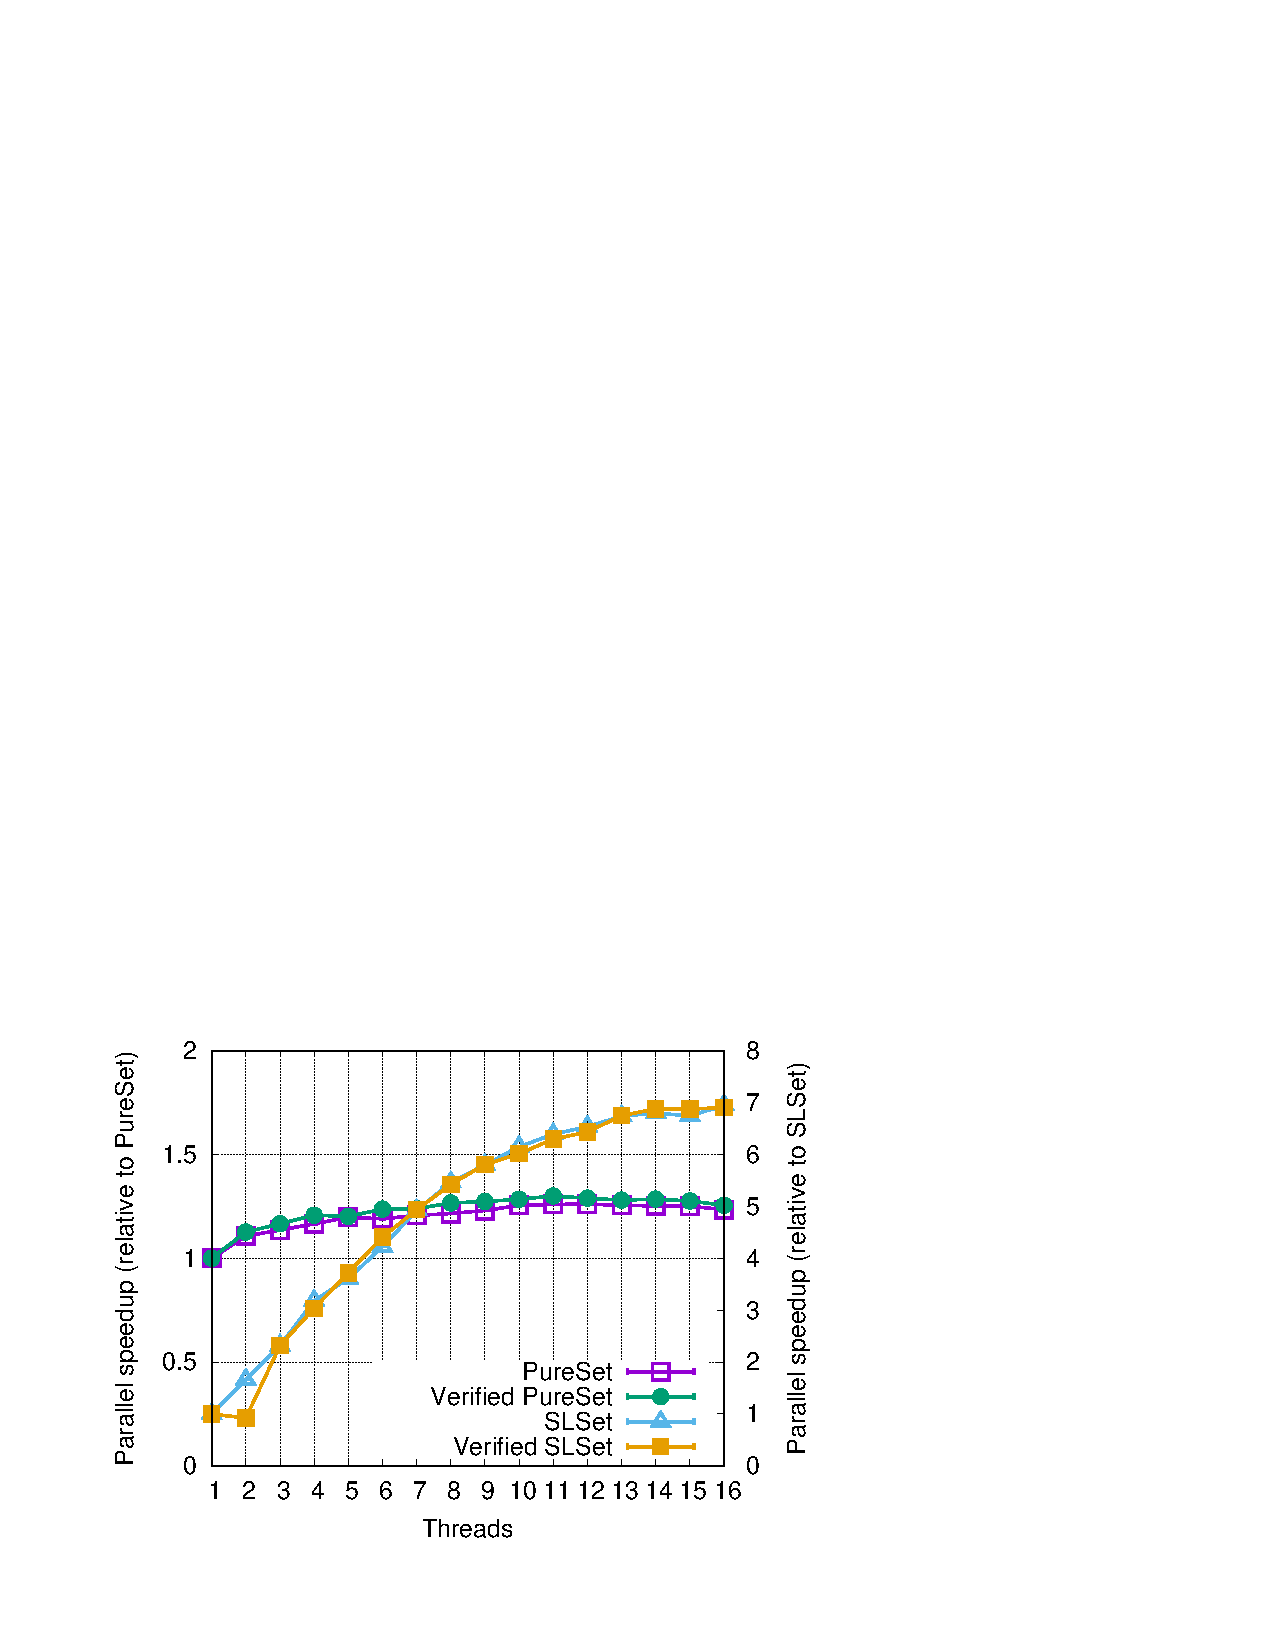
\includegraphics[width=3.7in]{../../data/set/set.pdf}
  \end{center}
  \caption{Parallel speedup for doing 1 million parallel inserts over 10
    iterations, verified and unverified, relative to the unverified version,
    for PureSet and SLSet.}
  \label{fig:set}
\end{figure}

\subsection{\texttt{monad-par}: $n$-body simulation}
\label{sec:nbody}
Next, we verify deterministic behavior of an
$n$-body simulation program that leverages @monad-par@, a Haskell library which
provides deterministic parallelism for pure code \cite{monad-par}.

Each simulated particle is represented by a
type @Body@ that stores its position, velocity, and mass.
%
The function @accel@ computes the relative acceleration
between two bodies:
\begin{mcode}
  accel :: Body -> Body -> Accel
\end{mcode}
where @Accel@ represents the three-dimensional acceleration
\begin{mcode}
  data Accel = $\texttt{Accel}$ Real Real Real
\end{mcode}
%
To compute the total acceleration
of a body @b@ we
(1) compute the relative acceleration between @b@
and each body of the system (@Vec Body@) and
(2) we add each acceleration component.
%
For efficiency, we use a parallel @mapReduce@ for the above
computation that
first \textit{maps} each vector body to get the acceleration relative to @b@
(@accel b@) and then adds each @Accel@ value by pointwise addition.
%
@mapReduce@ is only deterministic if the element is a @VerifiedMonoid@
from \S~\ref{sec:detpar}.
%%
%%To compute the velocity of each body in the simulation
%%we map reduce
%%
%%
%%An $n$-body simulation is used to model the behavior of particles in some system
%%in which forces are acting on the particles. The code which we verify is adapted
%%from an implementation of the all-pairs variant (a traditional, brute-force
%%approach) to $n$-body simulation from \cite{parallel-n-body}. The datatype which
%%we are verifying represents a particle:
%%
%%
\begin{mcode}
  mapReduce :: VerifiedMonoid b => (a -> b) -> Vec a -> b
\end{mcode}
%
To enforce the determinism of an $n$-body simulation, we need to provide a
@VerifiedMonoid@ instance for @Accel@.
%
We can prove that (@Real@, @+@, @0.0@)
is a monoid.
%
By product proof composition, we get a verified monoid instance for
\begin{mcode}
  type Accel' = (Real, (Real, Real))
\end{mcode}
which is isomorphic to @Accel@ (\ie @Iso Accel' Accel@).

Figure~\ref{fig:nbody} shows the results of running two versions of the $n$-body
simulation with 2,048 bodies over 5 iterations, with and without verification,
using floating point doubles for \texttt{Real}\footnote{Floating point numbers
  notoriously violate associativity, but we use this approximation because
  Haskell does net yet have an implementation of {\em
    superaccumulators}~\cite{superaccumulation}.}. Notably, the two programs have almost
identical runtime performance.  This demonstrates that even when verifying code
that is run in a tight loop (like @accel@), we can expect that our programs
will not be slowed down by an unacceptable amount.

\begin{figure}
  \begin{center}
    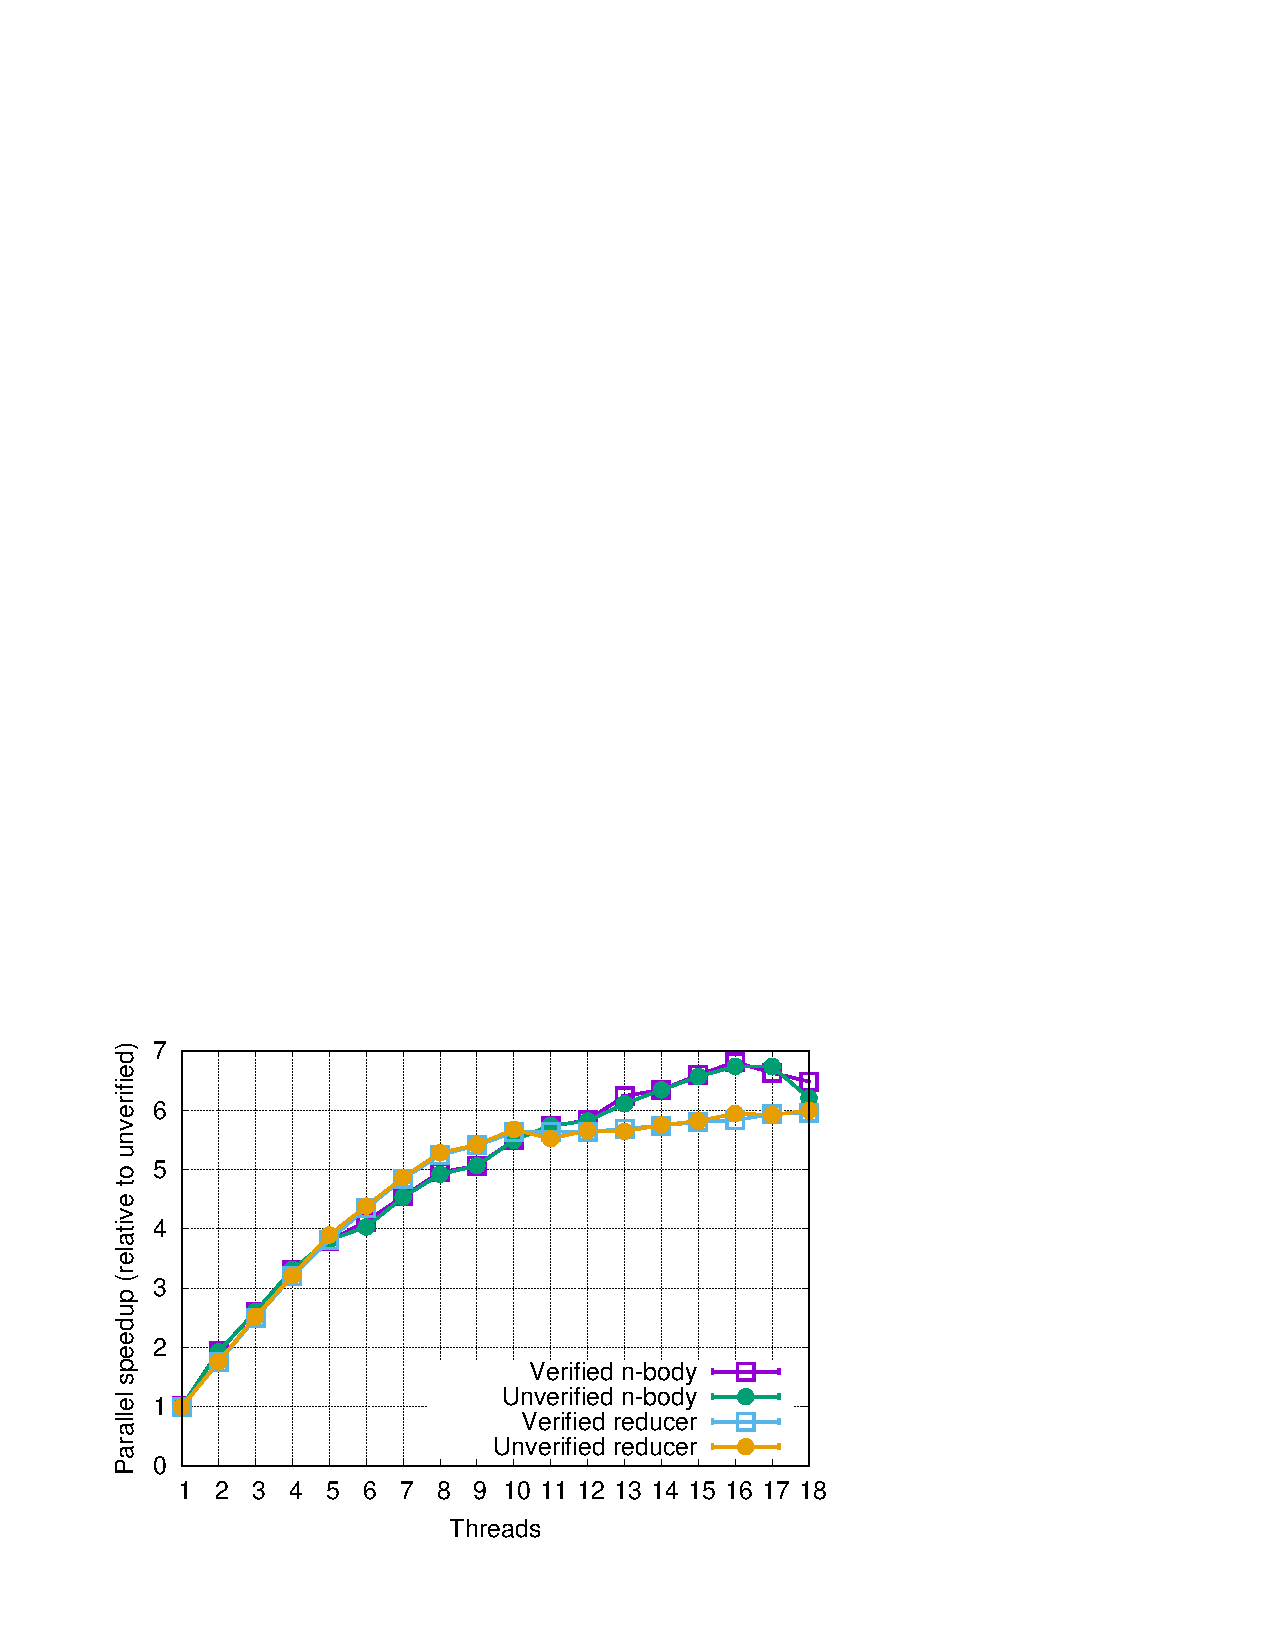
\includegraphics[width=3.7in]{../../data/nbody-reducer/nbody.pdf}
  \end{center}
  \caption{Parallel speedup for doing a parallel $n$-body simulation and
      parallel array reduction. The speedup is relative to the
    unverified version of each respective class of program.}
  \label{fig:nbody}
\end{figure}

\subsection{DPJ: Parallel Reducers}
\label{sec:reducer}
%% Our last benchmark illustrates how one can enforce various deterministic properties
%% that are different from the standard class properties (\ie monoid associativity).
%% For example,
The Deterministic Parallel Java (DPJ) project provides
a deterministic-by-default semantics for the Java programming language~\cite{DPJ}.
%
In DPJ, one can declare a method as @commutative@ and thus {\em assert} that
racing instances of that method result in a deterministic outcome.
For example:
%
% private region AccumRgn, static int sum in AccumRgn;
%% private static commutative synchronized
%%  void updateSum(int n) writes AccumRgn { sum += n; }
\begin{code}
  commutative void updateSum(int n) writes R { sum += n; }
\end{code}
But, DPJ provides no means to formally prove commutativity and thus
determinism of parallel reduction.
In Liquid Haskell, we specified commutativity as an extra proof method
that extends the @VerifiedMonoid@ class.
%
\begin{mcode}
  class VerifiedMonoid a => VerifiedCommutativeMonoid a where
    commutes :: x:a -> y:a -> { x <> y = y <> x }
\end{mcode}
%
Provably commutative appends can be used to deterministically
update a reducer variable, since the result is the same regardless
of the order of appends.
%
We used LVish~\cite{kuper2014freeze} to
encode a reducer variable with a value @a@ and a region @s@
as @RVar s a@.
\begin{mcode}
  newtype RVar s a
\end{mcode}
We specify that safe (\ie deterministic)
parallel updates require provably commutative appending.
\begin{mcode}
  updateRVar :: VerifiedCommutativeMonoid a => a -> RVar s a -> Par s ()
\end{mcode}
%
Following the DPJ program, we used @updateRVar@'s provably deterministic interface
to compute, in parallel, the sum of an array with $3$x$10^9$ elements by updating
a single, global reduction variable using a varying number of threads.
%
Each thread sums segments of an array, sequentially, and updates the variable
with these partial sums.
%
In Figure \ref{fig:nbody}, we compare the verified and unverified versions
of our implementation to observe no appreciable
difference in performance.

\section{Related Work}\label{sec:related}

% We compare refinement reflection to the most closely related
% lines of work in the vast literature on program verification.

\mypara{SMT-Based Verification}
%
SMT-solvers have been extensively used to automate
program verification via Floyd-Hoare logics~\cite{Nelson81}.
%
Our work is inspired by Dafny's Verified
Calculations~\citep{LeinoPolikarpova16},
a framework for proving theorems in
Dafny~\citep{dafny}, but differs in
%
(1)~our use of reflection instead of axiomatization and
(2)~our use of refinements to compose proofs.
%
Dafny, and the related \fstar~\citep{fstar}
which like \toolname, uses types to compose
proofs, offer more automation by translating
recursive functions to SMT axioms.
However, unlike reflection, this axiomatic
approach renders typechecking and verification
undecidable (in theory) and leads to
unpredictability and divergence
(in practice)~\citep{Leino16}.
%\NV{CHECL Relational-F*, Barthe et al, from POPL 2014, and EasyCrypt}

%% In a work more closely related to
%% ours, \fstar uses refinement types
%% for program verification supporting
%% expressiveness of fully dependent types.
%% %
%% As in Dafny, \fstar directly translates
%% recursive functions to axioms in the logic
%% thus suffers from the ``butterfly effect''
%% and allows the user to explicitly write SMT tactics to control it.

%% Leino \etal~\citep{Leino16}
%% name this problem as the ``butterfly
%% effect'', in which minor modifications
%% to the program source cause significant
%% instabilities in verification and propose
%% trigger selection strategies to address it.
%% %
%% We avoid the ``butterfly effect'' by not
%% directly axiomatizing functions into logic.
%% Instead the information about the function's
%% body is exactly captured in function's result
%% type and user needs to explicitly invoke the function to push
%% the function's definition information into the logic.


\mypara{Dependent types}
%
Our work is also inspired by dependently typed
systems like Coq~\citep{coq-book} and
Agda~\citep{agda}.
%
Reflection shows how deep specification
and verification in the style of Coq and Agda
can be \emph{retrofitted} into existing languages
via refinement typing.
%
Furthermore, we can use SMT to significantly
automate reasoning over important theories like
arithmetic, equality and functions.
%
It would be interesting to investigate how
the tactics and sophisticated proof search
of Coq \etc can be adapted to the refinement setting.

% which allow for arbitrary expressiveness of the type system
% in the cost of automatic verification.
%
%% The syntax of \libname's operators is inspired by
%% Equational Reasoning in Agda~\citep{agda}.
%% Here we extended these equational operators
%% to support linear arithmetic and, for example, prove
%% properties of Ackermann function.
%% %
%% Unlike Adga, proof term are explicit in \libname,
%% we do not use heuristics to infer proofs.


%%\mypara{Dependent Types for Non-Terminating Programs}
%%%
%%Zombie~\citep{Zombie, Sjoberg2015} integrates
%%dependent types in non terminating programs
%%and supports automatic reasoning for equality.
%%%
%%Vazou \etal have previously~\citep{Vazou14} shown
%%how Liquid Types can be used to check
%%non-terminating programs.
%%%
%%Reflection makes \toolname at least as
%%expressive as Zombie, \emph{without}
%%having to axiomatize the theory of
%%equality within the type system.
%%%
%%Consequently, in contrast to Zombie,
%%SMT based reflection lets \toolname
%%verify higher-order specifications
%%like @foldr_fusion@.

% which lets us use SMT automation
% to verify deep specifications of
% non-trivial programs.
%
% Our current extension is orthogonal to the
% previous work: our system remains sound as
% long as logical terms provably terminate.
%
% We get automation from SMT solvers for not only
% the theory of equality, but also linear arithmetic.
%
% \NV{Zombie with rewritting does not allow HIGHER ORDER reasoning}

\mypara{Dependent Types in Haskell}
%
Integration of dependent types into Haskell
has been a long standing goal that dates back
to Cayenne~\citep{cayenne}, a Haskell-like,
fully dependent type language with undecidable
type checking.
%
In a recent line of work~\citet{EisenbergS14}
aim to allow fully dependent
programming within Haskell, by making
``type-level programming ... at least as
  expressive as term-level programming''.
%
Our approach differs in two significant ways.
%
First, reflection allows SMT-aided verification,
which drastically simplifies proofs over key theories
like linear arithmetic and equality.
%
Second, refinements are completely erased at run-time.
That is, while both systems automatically lift Haskell
code to either uninterpreted logical functions
or type families, with refinements, the logical
functions are not accessible at run-time and
promotion cannot affect the semantics of
the program.
%
As an advantage (resp. disadvantage), refinements
cannot degrade (resp. optimize)
the performance of programs.

\mypara{Proving Equational Properties}
% of Haskell Programs}
%
Several authors have proposed tools for proving
(equational) properties of (functional) programs.
%
Systems~\citet{sousa16} and~\citet{KobayashiRelational15}
extend classical safety verification algorithms,
respectively based on Floyd-Hoare logic and Refinement Types,
to the setting of relational or $k$-safety properties
that are assertions over $k$-traces of a program.
%
Thus, these methods can automatically prove that
certain functions are associative, commutative \etc.
but are restricted to first-order properties and
are not programmer-extensible.
%
Zeno~\citep{ZENO} generates proofs by term
rewriting and Halo~\citep{HALO} uses an axiomatic
encoding to verify contracts.
%
Both the above are automatic, but unpredictable and not
programmer-extensible, hence, have been limited to
far simpler properties than the ones checked here.
%
HERMIT~\citep{Farmer15} proves equalities by rewriting
the GHC core language, guided by user specified scripts.
%
In contrast, our proofs are simply Haskell programs,
we can use SMT solvers to automate reasoning, and,
most importantly, we can connect the validity of
proofs with the semantics of the programs.

% \RJ{say: hermit does typeclass laws}
%
% \NV{TO ADD Naoki and class laws for TFP}
%
%% Compared to these systems, our proofs are
%% expressed as Haskell programs and do not
%% require the user to learn a different
%% tactic languages.
%% %
%% Moreover, our system is more general
%% as it allows for both equational
%% and linear arithmetic proofs.
%% %
%% On the other hand, \libname requires
%% explicit proofs and does not currently
%% support any automatic heuristics.

\mypara{Deterministic Parallelism}
%
Deterministic parallelism has plenty of theory but relatively few practical
implementations.  Early discoveries were based on limited producer-consumer
communication, such as single-assignment variables \cite{Tesler-1968,IStructures}, Kahn
process networks~\cite{kahn-1974}, and synchronous dataflow~\cite{lee-sdf}.
Other models use synchronous updates to shared state, as in
Esterel~\cite{synchronous-overview} or PRAM.  Finally, work on type systems for
permissions management \cite{permission-types,habanero-java-permissions},
supports the development of {\em non-interfering} parallel programs that access
disjoint subsets of the heap in parallel.  Parallel functional programming is
also non-interfering~\cite{manticore,multicore-ghc}.
%
Irrespective of which theory is used to support deterministic parallel
programming, practical implementations such as Cilk~\cite{cilk} or Intel
CnC~\cite{cnc} are limited by host languages with type systems insufficient to
limit side effects, much less prove associativity.  Conversely, dependently
typed languages like Agda and Idris do not have parallel programming APIs and
runtime systems.

% synchronous languages such as Esterel




\section{Conclusions and Future Work}

We have shown how refinement reflection---namely
reflecting the definitions of functions in their
output refinements---can be used to convert a
legacy programming language, like Haskell,
into a theorem prover.
%
Reflection ensures that (refinement) type checking
stays decidable and predictable via careful design
of the logic and proof combinators.
%
Reflection enables programmers working with
the highly tuned libraries, compilers and
run-times of legacy languages to specify
and verify arbitrary properties of their
code simply by writing programs in the
legacy language.
%
Our evaluation shows that refinement reflection
lets us prove deep specifications of a variety
of implementations, for example, the determinism
of fast parallel programming libraries, and also
identifies two important avenues for research.

First, while our proofs are often elegant
and readable, they can sometimes be cumbersome.
For example, in the proof of associativity of
the monadic bind operator for the @Reader@ monad
three out of eight (extensional) equalities required
explanations, some nested under multiple
$\lambda$-abstractions. Thus, it would be
valuable to explore how to extend the notions
of tactics, proof search, and automation
to the setting of legacy languages.
%
Similarly, while our approach to $\alpha$- and
$\beta$-equivalence is sound, we do not know
if it is \emph{complete}. We conjecture it is,
due to the fact that our refinement terms
are from the simply typed lambda calculus (STLC).
Thus, it would be interesting to use the
normalization of STLC to develop a sound
and complete system for SMT-based type-level
computation and use it to automate proofs
predictably.

Second, while Haskell's separation of pure
and effectful code undoubtedly makes it
easier to implement refinement reflection,
we believe that the technique, like
refinement typing in general, is orthogonal
to purity.
In particular, by carefully mediating
between the interaction of pure and
impure code using methods like
permissions, uniqueness \etc
refinement type systems have been
developed for legacy languages
like C \cite{LiquidPOPL10},
JavaScript \cite{Chugh2012, Vekris16},
and Racket \cite{RefinedRacket}
and so it would be interesting
to see how to extend refinement
reflection to other legacy languages.


%% \subsection*{Acknowledgements}

{
\bibliographystyle{plain}
\bibliography{sw}
}

\ifthenelse{\equal{\isTechReport}{true}}
{
\appendix
   \section{Implementation: \href{https://github.com/ucsd-progsys/liquidhaskell/tree/popl17}{Liquid Haskell}}

Refinement Reflection is fully implemented in
Liquid Haskell and will be included in the next release.
%
The implementation can be found in the
%
\href{https://git.io/vvARo}{Liquid Haskell GitHub repository},
%
all the benchmarks of \S~\ref{sec:overview} and~\S~\ref{sec:evaluation}
are included in the
%
\href{https://git.io/vXMKb}{tests},
the benchmarks of \S~\ref{sec:set}
are in the
\href{https://git.io/vXMKX}{LVars repo},
and the rest benchmarks of \S~\ref{sec:eval-parallelism}
are in the
\href{https://git.io/vXMKa}{verified-instances} repo.

%
Next, we describe the file
%
\href{https://github.com/ucsd-progsys/liquidhaskell/blob/pldi17/benchmarks/pldi17/pos/Proves.hs}{Proves.hs},
%
the library of proof combinators used by our benchmarks
and discuss known limitations of our implementation.


\renewcommand\libname{\ensuremath{\texttt{Proves}}\xspace}

\subsection{\libname: The Proof Combinators Library}
\label{subsec:library}

In this section we present \libname,
a Haskell library used to structure proof terms.
%
\libname is inspired by Equational Reasoning Data Types
in Adga~\citep{agdaequational}, providing operators to
construct proofs for equality and linear arithmetic in Haskell.
%
The constructed proofs are checked by an SMT-solver via Liquid Types.

\spara{Proof terms} are defined in \libname as a type alias for unit,
a data type that curries no run-time information
%
\begin{code}
  type Proof = ()
\end{code}
%
Proof types are refined to express theorems about program functions.
%
For example, the following @Proof@ type expresses that
@fib 2 == 1@
%
\begin{code}
  fib2 :: () -> {v:Proof | fib 2 == 1}
\end{code}
%
We simplify the above type by omitting the irrelevant
basic type @Proof@ and variable @v@
%
\begin{code}
  fib2 :: () -> { fib 2 == 1 }
\end{code}
%

\libname provides primitives to construct proof terms
by casting expressions to proofs.
%
To resemble mathematical proofs,
we make this casting post-fix.
%
We write @p *** QED@ to cast @p@ to a proof term,
by defining two operators @QED@ and @***@ as
%
\begin{code}
  data QED = QED

  (***) :: a -> QED -> Proof
  _ *** _  = ()
\end{code}

\spara{Proof construction.}
%
To construct proof terms, \libname
provides a proof constructor @op.@
for logical operators of the theory of
linear arithmetic and equality:
$\{=, \not =, \leq, <, \geq, > \} \in \odot$.
@op. x y@ ensures that $x \odot y$ holds, and returns @x@
%
\begin{code}
  op.:: x:a -> y:{a| x op y} -> {v:a| v==x}
  op. x _ = x

  -- for example
  ==.:: x:a -> y:{a| x==y} -> {v:a| v==x}
\end{code}
%
For instance, using @==.@
we construct a proof, in terms of Haskell code,
that @fib 2 == 1@:
%
\begin{code}
  fib2 _
    =   fib 2
    ==. fib 1 + fib 0
    ==. 1
    *** QED
\end{code} %$

\spara{Reusing proofs: Proofs as optional arguments.}
%
Often, proofs require reusing existing proof terms.
%
For example, to prove @fib 3 == 2@ we can reuse the above
@fib2@ proof.
%
We extend the proof combinators, to receive
an \textit{optional} third argument of @Proof@ type.
%
\begin{code}
  op.:: x:a -> y:a -> {x op y} -> {v:a|v==x}
  op. x _ _ = x
\end{code}
%
@op. x y p@ returns @x@ while the third argument @p@
explicitly proves $x \odot y$.

\spara{Optional Arguments.}
%
The proof term argument is optional.
To implement optional arguments in Haskell we use the standard technique
where for each operator @op!@ we define a type class @Optop@
that takes as input two expressions @a@ and returns a result @r@,
which will be instantiated with either the result value @r:=a@
or a function form a proof to the result @r:=Proof ->  a@.
%
\begin{code}
  class Optop a r where
    (op.) :: a -> a -> r
\end{code}
%
When no explicit proof argument is required,
the result type is just an @y:a@ that curries the proof @x op y@
%
\begin{code}
  instance Optop a a where
  (op.) :: x:a->y:{a| x op y}->{v:a | v==x }
  (op.) x _ = x
\end{code}
%
Note that Haskell's type inference~\citep{Sulzmann06}
requires both type class parameters @a@ and @r@ to be constrainted at class instance
matching time.
%
In most our examples, the result type parameter @r@ is not constrained
at instance matching time, thus
due to the Open World Assumption
the matching instance could not be determined.
%
To address the above, we used another common Haskell trick,
of generalizing the instance to type arguments @a@ and @b@ and then
constraint @a@ and @b@ to be equal @a~b@.
%
This generalization allows the instance to always match and
imposed the equality constraint after matching.
%
\begin{code}
  instance (a~b)=>Optop a b where
  (op.) :: x:a->y:{x op y}->{v:b | v==x }
  (op.) x _ = x
\end{code}


\begin{comment}
Explanation of (a~b) requirement

Function `foo` has the signature:

  foo :: Foo a r => a -> r

During type inference, the term `foo _5 True` gives rise to the wanted constraint:

WC = Foo Int (Bool -> b)
and the term has type: (foo _5 True) :: b

The top-level instance gives you the bidirectional CHR (simplification rule, if you
want to learn more about this check out "Understanding Functional Dependencies via
Constraint Handling Rules"):

  CHR: (a ~ b) <==> Foo a (Bool -> b)

Now, using the rule, you can replace your wanted constraint with (Int ~ b). This you
can now discharge by instantiating `b' to `Bool'. You may feel that instantiating `b'
is "random" but it is not. At this point is like HM, where you generate equality
constraints and search for a valid solution, and both `a' and `b' are universally
quantified.

The fact that the instance was picked is also not random: Your original instance head
imposes a non-structural restriction (non-linear pattern), so it is too restrictive,
but at the same time disallows you to give another similar instance to cover the
remaining similar cases (Foo a (Bool -> b) which would match the rest of the cases
where the `a's are not the same is no longer allowed, since they would overlap. Note
that GHC allows them both --even without OverlappingInstances enabled-- but this is
a bug #11605 :P). By being too restrictive, it cannot be picked (a and b have to be
checked for equality when matching, and during inference, this information is not there.
That is why the `bar' with signature `Int -> Bool' did not have this problem, indirectly
it fixes `b' to `Int' --and `a' is already `Int'-- so it can match).

  Foo a (Bool -> a) -- Your original instance head
  Foo a (Bool -> b) -- The updated instance head

Instead, your new instance head is the most general, and it matches ANYWAY, even without
knowing `b'.
\end{comment}
%
To explicitly provide a proof argument,
the result type @r@ is instantiated to @r:= Proof -> a@.
%
For the same instance matching restrictions as above,
the type is further generalized to return some @b@
that is constraint to be equal to @a@.
%
\begin{code}
  instance (a~b)=>Optop a (Proof->b) where
  (op.) :: x:a->y:a->{x op y}->{v:b | v==x }
  (op.) x _ _ = x
\end{code}
%
As a concrete example, we define the equality operator @==.@
via the type class @OptEq@ as
\begin{code}
  class OptEq a r where
   (==.):: a -> a -> r

  instance (a~b)=>OptEq a b where
   (==.)::x:a->y:{a|x==y}->{v:b|v==x}
   (==.) x _ = x

  instance (a~b)=>OptEq a (Proof->b) where
   (==.)::x:a->y:a->{x==y}->{v:b|v==x}
   (==.) x _ _ = x
\end{code}

\spara{Explanation Operator.}
%
The ``explanation operator'' @(?)@, or @($\because$)@,
is used to better structure the proofs.
%
@(?)@ is an infix operator with same fixity as @(op.)@
that allows for the equivalence
%
@ x op. y ? p == (op.) x y p@
%
\begin{code}
  (?) :: (Proof -> a) -> Proof -> a
  f ? y = f y
\end{code}

\spara{Putting it all together}
%
Using the above operators,
we prove that @fib 3 == 2@,
reusing the previous proof of @fib 2 == 1@,
in a Haskell term that resembles mathematical proofs
%
\begin{code}
  fib3 :: () ->  {fib 3 == 2}
  fib3 _
    =   fib 3
    ==. fib 2 + fib 1
    ==. 2             ? fib2 ()
    *** QED
\end{code}


\spara{Unverified Operators}
All operators in \libname, but two are implemented in Haskell
with implementations verified by Liquid Haskell.
%
The ''unsound`` operators are the assume
(1). @(==?)@ that eases proof construction by assuming equalities, to be proven later
and (2). @(=*)@ extentional proof equality.

\spara{Assume Operator} @(==?)@ eases proof construction by
assuming equalities while the proof is in process.
%
It is not implemented in that its body is @undefined@.
%
Thus, if we run proof terms including assume operator, the proof will merely crash
(instead of returning @()@).
%
Proofs including the assume operator are not considered complete,
as via assume operator any statement can be proven,

\spara{Function Extensional Equality}
Unlike the assume operator that is undefined and
included in unfinished thus unsound proofs,
the functions extensionality is included in valid proofs
that assume function extensionality, an axioms that is assumed,
as it cannot be proven by our logic.

To allow function equality via extensionality,
we provide the user with a function comparison operator
that for each function @f@ and @g@ it transforms a proof
that for every argument @x@, @f x = g x@ to a proof
on function equality @f = g@.
\begin{code}
(=*) :: Arg a => f:(a -> b) -> g:(a -> b)
     -> p:(x:a -> {f x = g x})
     -> {f = g}
\end{code}
%
The function @(=*)@ is not implemented in the library:
it returns () and its type is assumed.
%
But soundness of its usage requires the argument type variable @a@
to be constrained by a type class constraint @Arg a@,
for both operational and type theoretic reasons.
%

From \textit{operational} point of view,
an implementation of @(=*)@ would require checking
equality of @f x = g x@ \textit{forall} arguments @x@ of type @a@.
%
This equality would hold due to the proof argument @p@.
%
The only missing point is a way to enumerate all the argument @a@,
but this could be provided by a method of the type clas @Arg a@.
%
Yet, we have not implement @(=*)@ because we do not know how to
provide such an implementation that can provably satisfy @(=*)@'s type.

From \textit{type theoretic} point of view,
the type variable argument @a@
appears only on negative positions.
%
Liquid type inference is smart enough to infer that
since @a@ appears only negative @(=*)@ cannot use any @a@
and thus will not call any of its argument arguments @f@, @g@, nor the @p@.
%
Thus, at each call site of @(=*)@ the type variable `a` is instantiated
with the refinement type @{v:a | false}@ indicating dead-code
(since @a@s will not be used by the callee.)
%
Refining the argument @x:a@ with false at each call-site though
leads to unsoundness, as each proof argument @p@ is a valid proof under
the false assumption.
%
What Liquid inference cannot predict is our intention to call
@f@, @g@ and @p@ at \textit{every possible argument}.
%
This information is capture by the type class constraint @Arg a@
that (as discussed before~\citep{Vazou13}) states that methods of
the type class
@Arg a@ may create values of type @a@, thus,
due to lack of information on the values that are created by the
methods of @Arg a@, @a@ can only be refined with @True@.

With extensional equality, we can prove
that @\x -> x@ is equal to @\x -> id x@,
by providing an explicit explanation that
if we call both these functions with the same
argument @x@, they return the same result, for each @x@.
%
\begin{mcode}
 safe :: Arg a => a
       -> {(\x -> id x) = (\x -> x)}
 safe _  = (\x -> x)
         =*(\x -> id x) $\because$ (exp ())

 exp :: Arg a => a -> x:a
     -> {(\x -> id x) x = (\x -> x) x}
 exp _ x =  id x
         ==. x
         *** QED
\end{mcode}
%
Note that the result of @exp@
is an equality of the redexes
@(\x -> id x) x@ and @((\x -> x) x@.
%
Extentional function equality requires
as argument an equality on such redexes.
%
Via $\beta$ equality instantiations,
both such redexes will automatically reduce,
requiring @exp@ to prove @id x = x@,
with is direct.

Admittedly, proving function equality via extensionality
is requires a cumbersome indirect proof.
%
For each function equality in the main proof
one needs to define an explanation function
that proves the equality for every argument.


\subsection{Engineering Limitations}
The theory of refinement reflection is fully implemented in Liquid Haskell.
%
Yet, to make this extension \textit{usable} in \textit{real world applications}
there are four known engineering limitations that need to be addressed.
%
All these limitations seem straightforward to address
and we plan to fix them soon.

\spara{The language of refinements}
is typed lambda calculus. That is the types of the lambda arguments are
explicitly specified
instead of being inferred.
%
As another minor limitation, the refinement language parser
requires the argument to be enclosed in parenthesis
in applications where the function is not a variable.
%
Thus the Haskell expression
@(\x -> x) e@ should be written as @(\x:a -> x) (e)@
in the refinement logic,

\spara{Class instances methods} can not be reflected.
%
Instead, the methods we want to use in the theorems/propositions
should be defined as Haskell functions.
%
This restriction has two major implications.
%
Firstly, we can not verify correctness of library provided
instances but we need to redifine them ourselves.
%
Secondly, we cannot really verify class instances with class preconditions.
%
For example, during verification of monoid associativity of the Maybe instance
\begin{code}
  instance (Monoid a) => Monoid (Maybe a)
\end{code}
%
there is this @Monoid a@ class constraint assumption we needed to raise to
proceed verification.

\spara{Only user defined data types}
can currently used in verification.
%
The reason for this limitation is that
reflection of case expressions
requires checker and projector measures for each
data type used in reflected functions.
%
Thus, not only should these data types be defined in
the verified module, but also should be
be injected in the logic by providing a refined version of
the definition that can (or may not) be trivially refined.

For example, to reflect a function that uses
@Peano@ numbers, the Haskell \textit{and} the refined @Peano@
definitions should be provided
%
\begin{code}
data Peano = Z | S Peano

{-@ data Peano [toInt]
     = Z
     | S {prev :: Peano}
  @-}
\end{code}
%
Note that the termination function @toInt@
that maps @Peano@ numbers to natural numbers
is also crucial for soundness of reflection.

\spara{There is no module support.}
All reflected definitions,
including, measures (automatically generated checkers and selector,
but also the classic lifted Haskell functions to measures)
and the reflected types of the reflected functions,
are not exposed outside of the module they are defined.
%
Thus all definitions and propositions should exist in the same module.

   \section{Refinement Reflection: \corelan: Extended Version with Proofs}
\label{sec:appendix:formalism}
\label{sec:appendix:types-reflection}

Our first step towards formalizing refinement
reflection is a core calculus \corelan with an
\emph{undecidable} type system based on
denotational semantics.
We show how the soundness of the type system
allows us to \emph{prove theorems} using \corelan.

%
%% Note that \smtlan programs are a subset of
%% \corelan programs derivations
%%
%% a subset of \corelan where the that forms a
%% decidable logic of
%% refinements, and use it to obtain \corelan with
%% decidable SMT-based algorithmic typing.

\subsection{Syntax}
\begin{figure}[t!]
\centering
$$
\begin{array}{rrcl}
\emphbf{Operators} \quad
  & \odot
  & ::= & = \spmid  <
\\[0.03in]

\emphbf{Constants} \quad
  & c
  & ::=
  & \land \spmid \lnot \spmid \odot \spmid +,-,\dots  \\
  && \spmid & \etrue\spmid \efalse \spmid 0, 1,-1, \dots
\\[0.03in]

\emphbf{Values} \quad
  & w & ::=&  c
             \spmid \efun{x}{\typ}{e} \spmid D\ \overline{w}
\\[0.03in]

\emphbf{Expressions} \quad
  & e & ::=    & w \spmid x \spmid \eapp{e}{e}      \\
  &   & \spmid & \ecase{x}{e}{\dc}{\overline{x}}{e}
  %% &   & \spmid & \eletb{x}{\gtyp}{e}{e}
\\[0.03in]

\emphbf{Binders} \quad
  & \bd & ::= & e \spmid \eletb{x}{\gtyp}{\bd}{\bd}
\\[0.03in]

\emphbf{Program} \quad
  & \prog & ::= & \bd \spmid \erefb{x}{\gtyp}{e}{\prog}
\\[0.03in]

% \emphbf{Logical Labels} \quad
%  & L & ::= & \la \spmid \lm
%\\[0.03in]

\emphbf{Basic Types} \quad
  & \btyp
  & ::=
  & \tint \spmid \tbool \spmid T
\\[0.03in]

\emphbf{Refined Types} \quad
  & \typ
  & ::=      & \tref{v}{\btyp}{\reft} \spmid \tfun{x}{\typ}{\typ}
\\[0.05in]
\end{array}
$$
\caption{\textbf{Syntax of \corelan}}
\label{fig:appendix:syntax}
\end{figure}

\begin{figure}[t!]
\centering

\emphbf{Contexts}\hfill{{$\fbox{\textit{C}}$}}
$$
\begin{array}{rcl}
  C & ::=    & \bullet \\
    & \spmid & C\ e \spmid c\ C \spmid D\ \overline{e}\ C\ \overline{e}\\
    & \spmid & \ecase{y}{C}{\dc_i}{\overline{x}}{e_i}
  \\[0.03in]
\end{array}
$$

\emphbf{Reductions}\hfill{{$\fbox{\goesto{\prog}{\prog'}}$}}
$$
\begin{array}{rcl}
C[\prog]
  & \hookrightarrow
  & C[\prog'],\quad \text{if}\ \goesto{\prog}{\prog'}
  \\
{c\ v}
  & \hookrightarrow
  & {\ceval{c}{v}}
  \\
{({\efun{x}{\typ}{e})}\ {e'}}
  & \hookrightarrow
  & {\SUBST{e}{x}{e'}}
  \\
{\ecase{y}{\dc_j\ \overline{e}}{\dc_i}{\overline{x_i}}{e_i}}
  & \hookrightarrow
  & {\SUBST{\SUBST{e_j}{y}{\dc_j\ \overline{e}}}{\overline{x_i}}{\overline{e}}}
  \\
{\erefb{x}{\gtyp}{e}{\prog}}
  & \hookrightarrow
  & {\SUBST{\prog}{x}{\efix{(\efun{x}{\gtyp}{e})}}}
  \\
{\eletb{x}{\gtyp}{\bd_x}{\bd}}
  & \hookrightarrow
  % & {\SUBST{\prog}{x}{e}}
  & {\SUBST{\bd}{x}{\efix{(\efun{x}{\gtyp}{\bd_x})}}}
  \\
%% {\eletrec{x}{e_x}{\gtyp}{[L]}{\prog}}
  %% & \hookrightarrow
  %% & {\SUBST{\prog}{x}{\efix{\efun{x}{\gtyp}{e_x}}}}
  %% \\
{\efix{\prog}}
  & \hookrightarrow
  & {\prog\ (\efix{\prog})}
\end{array}
$$
\caption{\textbf{Operational Semantics of \corelan}}
\label{fig:semantics}
\end{figure}

%
Figure~\ref{fig:appendix:syntax} summarizes the syntax of \corelan,
which is essentially the calculus \undeclang~\cite{Vazou14}
with explicit recursion and a special $\erefname$ binding form
to denote terms that are reflected into the refinement logic.
%
In \corelan refinements $r$ are arbitrary expressions $e$
(hence $r ::= e$ in Figure~\ref{fig:appendix:syntax}).
%
This choice allows us to prove preservation and progress,
but renders typechecking undecidable.
%
In \S~\ref{sec:appendix:algorithmic} we will see how to recover
decidability by soundly approximating refinements.

The syntactic elements of \corelan are layered into
primitive constants, values, expressions, binders
and programs.

\mypara{Constants}
The primitive constants of \corelan
include all the primitive logical
operators $\op$, here, the set $\{ =, <\}$.
%
Moreover, they include the
primitive booleans $\etrue$, $\efalse$,
integers $\mathtt{-1}, \mathtt{0}$, $\mathtt{1}$, \etc,
and logical operators $\mathtt{\land}$, $\mathtt{\lor}$, $\mathtt{\lnot}$, \etc.

\mypara{Data Constructors}
%
We encode data constructors as special constants.
% Each data type has an equality predicate $\haseq{T}$
% that is true only if values of type $T$ can be finitely compared.
For example the data type \tintlist, which represents
finite lists of integers, has two data constructors: $\dnull$ (``nil'')
and $\dcons$ (``cons'').
% and satisfies $\haseq{\tintlist}$.

%% NV Arity is not used anywhere
%%Each data type has an arity $\arity{T}$ that represents
%%the exact number of data constructors that return
%%a value of type $T$.
%
%%For example the data type \tintlist, which represents
%%lists of integers, has two data constructors: $\dnull$ (``nil'')
%%and $\dcons$ (``cons'') and so has arity $2$.


\mypara{Values \& Expressions}
%
The values of \corelan include
constants, $\lambda$-abstractions
$\efun{x}{\typ}{e}$, and fully
applied data constructors $D$
that wrap values.
%
The expressions of \corelan
include values and variables $x$,
applications $\eapp{e}{e}$, and
$\mathtt{case}$ expressions.

\mypara{Binders \& Programs}
%
A \emph{binder} $\bd$ is a series of possibly recursive
let definitions, followed by an expression.
%
A \emph{program} \prog is a series of $\erefname$
definitions, each of which names a function
that can be reflected into the refinement
logic, followed by a binder.
%
The stratification of programs via binders
is required so that arbitrary recursive definitions
are allowed but cannot be inserted into the logic
via refinements or reflection.
%
(We \emph{can} allow non-recursive $\mathtt{let}$
binders in $e$, but omit them for simplicity.)

\subsection{Operational Semantics}

Figure~\ref{fig:appendix:syntax} summarizes the small
step contextual $\beta$-reduction semantics for
\corelan.
%
%%There are two points to note.
%%%
%%First, we allow for reductions under
%%data constructors, and thus, values may
%%be further reduced.
%%%
%%Second, for simplicity, we treat both
%%$\eletname$ and $\erefname$ as possibly
%%recursive (\ie $\mathtt{let\ rec}$) binders.
%% Note that, for simplicity, we treat each
%% $\eletname$ as a possibly
%% recursive (\ie $\mathtt{let\ rec}$) binder.
%
We write \evalj{e}{e'}{j} if there exist
$e_1,\ldots,e_j$ such that $e$ is $e_1$,
$e'$ is $e_j$ and $\forall i,j, 1 \leq i < j$,
we have $\evals{e_i}{e_{i+1}}$.
%
We write $\evalsto{e}{e'}$ if there exists
some finite $j$ such that $\evalj{e}{e'}{j}$.
%
We define $\betaeq{}{}$ to be the reflexive,
symmetric, transitive closure of $\evals{}{}$.

\mypara{Constants} Application of a constant requires the
argument be reduced to a value; in a single step the
expression is reduced to the output of the primitive
constant operation.
%
For example, consider $=$, the primitive equality
operator on integers.
%
We have $\ceval{=}{n} \defeq =_n$
where $\ceval{=_n}{m}$ equals \etrue
iff $m$ is the same as $n$.
%
%\mypara{Equality}
%
We assume that the equality operator
is defined \emph{for all} values,
and, for functions, is defined as
extensional equality.
%
That is, for all
$f$ and
$f'$
we have
$\evals{(f = f')}{\etrue}
  \quad \mbox{iff} \quad
  \forall v.\ \betaeq{f\ v}{f'\ v}$.
%
We assume source \emph{terms} only contain implementable equalities
over non-function types; the above only appears in \emph{refinements}
and allows us to state and prove facts about extensional
equality~\S~\ref{subsec:extensionality}.
%% % \RJ{CHECK}

%%That is, for all
%%$f \defeq \efun{x}{\typ}{e}$ and
%%$f' \defeq \efun{x}{\typ}{e'}$
%%we have
%%$$\evals{(f = f')}{\etrue}
%%  \quad \mbox{iff} \quad
%%  \forall v.\ \evalsto{(\SUBST{e}{x}{v} = \SUBST{e'}{x}{v})}{\etrue}
%%$$


\subsection{Types}

\corelan types include basic types, which are \emph{refined} with predicates,
and dependent function types.
%
\emph{Basic types} \btyp comprise integers, booleans, and a family of data-types
$T$ (representing lists, trees \etc.)
%
For example the data type \tintlist represents lists of integers.
%
We refine basic types with predicates (boolean valued expressions \refa) to obtain
\emph{basic refinement types} $\tref{v}{\btyp}{\refa}$.
%
Finally, we have dependent \emph{function types} $\tfun{x}{\typ_x}{\typ}$
where the input $x$ has the type $\typ_x$ and the output $\typ$ may
refer to the input binder $x$.
%
We write $\btyp$ to abbreviate $\tref{v}{\btyp}{\etrue}$,
and \tfunbasic{\typ_x}{\typ} to abbreviate \tfun{x}{\typ_x}{\typ} if
$x$ does not appear in $\typ$.
%
We use $r$ to refer to refinements.


\mypara{Denotations}
%
Each type $\typ$ \emph{denotes} a set of expressions $\interp{\typ}$,
that are defined via the dynamic semantics~\cite{Knowles10}.
%
Let $\shape{\typ}$ be the type we get if we erase all refinements
from $\typ$ and $\bhastype{}{e}{\shape{\typ}}$ be the
standard typing relation for the typed lambda calculus.
%
Then, we define the denotation of types as:
\begin{align*}
\interp{\tref{x}{\btyp}{r}} \defeq &
    \{e \mid  \bhastype{}{e}{\btyp},
              \mbox{ if } \evalsto{e}{w}
              \mbox{ then } \evalsto{r\subst{x}{w}}{\etrue} \}\\
\interp{\tfun{x}{\typ_x}{\typ}} \defeq &
    \{e \mid  \bhastype{}{e}{\shape{\tfunbasic{\typ_x}{\typ}}},
              \forall e_x \in \interp{\typ_x}.\ \eapp{e}{e_x} \in \interp{\typ\subst{x}{e_x}}
    \}
\end{align*}


\mypara{Constants}
For each constant $c$ we define its type \constty{c}
such that $c \in \interp{\constty{c}}$.
%
For example,
%
$$
\begin{array}{lcl}
\constty{3} &\doteq& \tref{v}{\tint}{v = 3}\\
\constty{+} &\doteq& \tfun{\ttx}{\tint}{\tfun{\tty}{\tint}{\tref{v}{\tint}{v = x + y}}}\\
\constty{\leq} &\doteq& \tfun{\ttx}{\tint}{\tfun{\tty}{\tint}{\tref{v}{\tbool}{v \Leftrightarrow x \leq y}}}\\
\end{array}
$$
%
So, by definition we get the constant typing lemma
%
\begin{lemma}{[Constant Typing]}\label{lemma:constants}
Every constant $c \in \interp{\constty{c}}$.
\end{lemma}
%
Thus, if $\constty{c} \defeq \tfun{x}{\typ_x}{\typ}$,
then for every value $w \in \interp{\typ_x}$, we require
$\ceval{c}{w} \in \interp{\typ\subst{x}{w}}$.

%% \mypara{Equality}
%% The equality predicate
%% $\haseq{B}$, is defined to be true for \tint and \tbool,
%% and for each type constructor $T$
%% whose values can be finitely compared.
%% %
%% So, by definition we get the equality lemma
%% %
%% \begin{lemma}{[Equality]}\label{lemma:equality}
%% If $\haseq{B}$ then for each value $\bhastype{\emptyset}{w}{B}$
%% \evalsto{w = w}{\etrue}
%% \end{lemma}

\subsection{Refinement Reflection}
\label{subsec:appendix:logicalannotations}
%
The simple, but key idea in our work is to
\emph{strengthen} the output type of functions
with a refinement that \emph{reflects} the
definition of the function in the logic.
%
We do this by treating each
%
$\erefname$-binder:
%
${\erefb{f}{\gtyp}{e}{\prog}}$
%
as a $\eletname$-binder:
%
${\eletb{f}{\exacttype{\gtyp}{e}}{e}{\prog}}$
%
during type checking (rule $\rtreflect$ in Figure~\ref{fig:typing}).

\mypara{Reflection}
%
We write \exacttype{\typ}{e} for the \emph{reflection}
of term $e$ into the type $\typ$,  defined by strengthening
\typ as:
%
$$
\begin{array}{lcl}
\exacttype{\tref{v}{\btyp}{r}}{e}
  & \defeq
  & \tref{v}{\btyp}{r \land v = e}\\
\exacttype{\tfun{x}{\typ_x}{\typ}}{\efun{y}{}{e}}
  & \defeq
  & \tfun{x}{\typ_x}{\exacttype{\typ}{e\subst{y}{x}}}
\end{array}
$$
%
As an example, recall from \S~\ref{sec:overview}
that the "reflect fib " strengthens the type of
"fib" with the reflected refinement "fibP".
%% NV In Overview, we have fibP v n = v = fib n && fibR v n
%% NV Here we get the reflection part (fibR v n)
%% NV which we can verify
%% NV at each fix invocation we also get the v = fib n portion
%% NV via the exact rule
%% NV We can not add the v = fib n as a port condition, because
%% NV we cannot prove it.


\mypara{Consequences for Verification}
%
Reflection has two consequences for verification.
%
First, the reflected refinement is \emph{not trusted};
it is itself verified (as a valid output type)
during type checking.
%
Second, instead of being tethered to quantifier
instantiation heuristics or having to program
``triggers'' as in Dafny~\citep{dafny} or
\fstar~\citep{fstar}
%
the programmer can predictably ``unfold'' the
definition of the function during a proof simply
by ``calling'' the function, which we have found
to be a very natural way of structuring
proofs~\S~\ref{sec:evaluation}.


\subsection{Refining \& Reflecting Data Constructors with Measures}
\label{subsec:appendix:measures}
\label{subsec:list}

% We reuse the notion of \emph{measures}~\cite{Vazou14}
% to reflect functions over datatypes into the refinement
% logic.

We assume that each data type is equipped with
a set of \emph{measures} which are \emph{unary}
functions whose (1)~domain is the data type, and
(2)~body is a single case-expression over the
datatype~\cite{Vazou14}:
%
$$\emeasb{f}
         {\gtyp}
         {\efun{x}{\typ}{\ecase{y}{x}{\dc_i}{\overline{z}}{e_i}}}$$
%
For example, "len" measures the size of an $\tintlist$:
%
\begin{code}
  measure len :: [Int] -> Nat
  len = \x -> case x of
                []     -> 0
                (x:xs) -> 1 + len xs
\end{code}

\mypara{Checking and Projection}
%
We assume the existence of measures that
\emph{check} the top-level constructor,
and \emph{project} their individual fields.
%
%\NV{Remove this pointer since we removed the text}
In \S~\ref{subsec:appendix:embedding} we show how to
use these measures to reflect functions over
datatypes.
%
% Such measures are straightforward to generate
% automatically from the data-type definition.)
%
For example, for lists, we assume the existence of measures:
%
\begin{code}
  isNil []      = True
  isNil (x:xs)  = False

  isCons (x:xs) = True
  isCons []     = False

  sel1 (x:xs)   = x
  sel2 (x:xs)   = xs
\end{code}

\mypara{Refining Data Constructors with Measures}
%
We use measures to strengthen the types
of data constructors, and we use these
strengthened types during construction
and destruction (pattern-matching).
%
Let:
%
(1)~$\dc$ be a data constructor,
   with \emph{unrefined} type
   $\tfun{\overline{x}}{\overline{\gtyp}}{T}$
%
(2)~the $i$-th measure definition with
   domain $T$ is:
%
$$\emeasb{f_i}
         {\gtyp}
         {\efun{x}{\typ}{\ecase{y}{x}{\dc}{\overline{z}}{e_{i}}}}
$$
%
Then, the refined type of $\dc$ is defined:
$$
\constty{\dc} \defeq
   \tfun{\overline{x}}
        {\overline{\typ}}
        {\tref{v}{T}{ \wedge_i f_i\ v = \SUBST{e_{i}}{\overline{z}}{\overline{x}}}}
$$

Thus, each data constructor's output type is refined to reflect
the definition of each of its measures.
%
For example, we use the measures "len", "isNil", "isCons", "sel1",
and "sel2" to strengthen the types of $\dnull$ and $\dcons$ to:
%
\begin{align*}
\constty{\dnull}  \defeq & \tref{v}{\tintlist}{r_{\dnull}} \\
\constty{\dcons}  \defeq & \tfun{x}{\tint}
                                   {\tfun{\mathit{xs}}
                                         {\tintlist}
                                         {\tref{v}{\tintlist}{r_\dcons}}}
\intertext{where the output refinements are}
r_{\dnull} \defeq &\ \mathtt{len}\ v = 0
             \land  \mathtt{isNil}\ v
             \land  \lnot \mathtt{isCons}\ v \\
r_{\dcons} \defeq &\ \mathtt{len}\ v = 1 + \mathtt{len}\ \mathit{xs}
             \land  \lnot \mathtt{isNil}\ v
             \land  \mathtt{isCons}\ v \\
             \land & \  \mathtt{sel1}\ v = x
             \land  \mathtt{sel2}\ v = \mathit{xs}
\end{align*}
%
It is easy to prove that Lemma~\ref{lemma:constants}
holds for data constructors, by construction.
%
For example, $\mathtt{len}\ \dnull = 0$ evaluates to $\tttrue$.


%%
%% The above annotation \emph{strengthens} the types of data constructors
%% $\dc_i$ to reflect the
%% behavior of $f$:
%%
%%
%% \preproc{\eletrecoptsmall{f}{\efun{x}{\typ}{\ecase{y}{x}{\dc_i}{\overline{z}}{e_i}}}{\gtyp}{M}{\prog}}
%%
%% %
%% Where \exacttypefun{f}{\gtyp}{e} strengthens the result $v$ of the type \typ to exactly
%% describe that $f\ v = e$:
%% %
%% \begin{align*}
%% \exacttypefun{f}{\tref{v}{\btyp}{r}}{e} &= \tref{v}{\btyp}{r \land f\ v = e}\\
%% \exacttypefun{f}{\tfun{x}{\typ_x}{\typ}}{\efun{y}{}{e}} &=\tfun{x}{\typ_x}{\exacttype{\typ}{e\subst{y}{x}}}
%% \end{align*}

\subsection{Typing Rules}
\begin{figure}[!t]
\emphbf{Typing}\hfill{\fbox{\hastype{\env}{\prog}{\typ}}}\\
$$
\inference{
	\tbind{x}{\gtyp}\in\env
}{
	\hastype{\env}{x}{\gtyp}
}[\rtvar]
\qquad
\inference{
}{
	\hastype{\env}{c}{\constty{c}}
}[\rtconst]
$$

$$
\inference{
	\hastype{\env}{\prog}{\typ'} &
	\issubtype{\env}{\typ'}{\typ}
}{
	\hastype{\env}{\prog}{\typ}
}[\rtsub]
$$
$$
\inference{
    % \haseq{\btyp} &
	\hastype{\env}{e}{\tref{v}{\btyp}{\reft_r}}
}{
	\hastype{\env}{e}{\tref{v}{\btyp}{\reft_r\land v = e}}
}[\rtexact]
$$
$$
\inference{
	\hastype{\env, \tbind{x}{\typ_x}}{e}{\typ}
}{
	\hastype{\env}{\efun{x}{\typ}{e}}{\tfun{x}{\typ_x}{\typ}}
}[\rtfun]
$$

$$
\inference{
	\hastype{\env}{e_1}{(\tfun{x}{\typ_x}{\typ})} &&
	\hastype{\env}{e_2}{\typ_x}
}{
	\hastype{\env}{e_1\ e_2}{\typ}
}[\rtapp]
$$

$$
\inference
	{\hastype{\env, \tbind{x}{\gtyp_x}}{\bd_x}{\gtyp_x} &
	 \iswellformed{\env, \tbind{x}{\gtyp_x}}{\typ_x} \\
	 \hastype{\env, \tbind{x}{\gtyp_x}}{\bd}{\gtyp} &
	 \iswellformed{\env}{\typ}}
	{\hastype{\env}{\eletb{x}{\gtyp_x}{\bd_x}{\bd}}{\typ}}
	[\rtlet]
$$

$$
\inference
	{\hastype{\env}
	 				 {\eletb{f}{\exacttype{\gtyp_f}{e}}{e}{\prog}}
					 {\typ}
	}
	{\hastype{\env}
					 {\erefb{f}{\gtyp_f}{e}{\prog}}
					 {\typ}
	}[\rtreflect]
$$

$$
\inference{
	\hastype{\env}{e}{\tref{v}{T}{e_r}} & \iswellformed{\env}{\typ} \\
	& \forall i. \constty{\dc_i} = \tfunbasic{\overline{\tbind{y_j}{\typ_j}}}{\tref{v}{T}{e_{r_i}}} \\
	& \hastype{\env, \overline{\tbind{y_j}{\typ_j}}, \tbind{x}{\tref{v}{T}{e_r \land e_{r_i}}} }{e_i}{\typ}
}{
	\hastype{\env}{\ecase{x}{e}{\dc_i}{\overline{y_i}}{e_i}}{\typ}
}[\rtcase]
$$
\emphbf{Well Formedness}\hfill{\fbox{\iswellformed{\env}{\typ}}}\\

$$
\inference{
  \hastype{\env,\tbind{v}{\btyp}}{\refa}{\tbool^{\tlabel}}
}{
	\iswellformed{\env}{\tref{v}{\btyp}{\refa}}
}[\rwbase]
$$
$$
\inference{
	\iswellformed{\env}{\typ_x} &
	\iswellformed{\env,\tbind{x}{\typ_x}}{\typ}
}{
	\iswellformed{\env}{\tfun{x}{\typ_x}{\typ}}
}[\rwfun]
$$

\emphbf{Subtyping}\hfill{\fbox{\issubtype{\env}{\typ_1}{\typ_2}}}\\

$$
\inference{
\env' \defeq \env,\tbind{v}{\{\btyp^\tlabel | \refa\}} \\
\tologicshort{\env'}{\refa'}{\tbool}{\pred'}{}{}{} &
\smtvalid{\vcond{\env'}{\pred'}}
%%	\forall \sub\in\interp{\env}.
%%	\interp{\applysub{\sub}{\tref{v}{\btyp}{\refa_1}}}
%%	\subseteq
%%	\interp{\applysub{\sub}{\tref{v}{\btyp}{\refa_2}}}
}{
	\issubtype{\env}{\tref{v}{\btyp}{\refa}}{\tref{v}{\btyp}{\refa'}}
}[\rsubbase]
$$

$$
\inference{
	\issubtype{\env}{\typ_x'}{\typ_x} &
	\issubtype{\env,\tbind{x}{\typ_x'}}{\typ}{\typ'}
}{
	\issubtype{\env}{\tfun{x}{\typ_x}{\typ}}{\tfun{x}{\typ_x'}{\typ'}}
}[\rsubfun]
$$
\caption{Typing of \corelan}
\label{fig:typing}
\end{figure}
%
Next, we present the type-checking
judgments and rules of \corelan.

\mypara{Environments and Closing Substitutions}
A \emph{type environment} $\env$ is a sequence of type bindings
$\tbind{x_1}{\typ_1},\ldots,\tbind{x_n}{\typ_n}$. An environment
denotes a set of \emph{closing substitutions} $\sto$ which are
sequences of expression bindings:
$\gbind{x_1}{e_1}, \ldots, \gbind{x_n}{e_n}$ such that:
$$
\interp{\env} \defeq  \{\sto \mid \forall \tbind{x}{\typ} \in \Env.
                                    \sto(x) \in \interp{\applysub{\sto}{\typ}} \}
$$

\mypara{Judgments}
We use environments to define three kinds of
rules: Well-formedness, Subtyping,
and Typing~\citep{Knowles10,Vazou14}.
%
%\mypara{Well-formedness}
A judgment \iswellformed{\env}{\typ} states that
the refinement type $\typ$ is well-formed in
the environment $\env$.
%
Intuitively, the type $\typ$ is well-formed if all
the refinements in $\typ$ are $\tbool$-typed in $\env$.
%
%\mypara{Subtyping}
A judgment \issubtype{\env}{\typ_1}{\typ_2} states
that the type $\typ_1$ is a subtype of %the type
$\typ_2$ in the environment $\env$.
%
Informally, $\typ_1$ is a subtype of $\typ_2$ if, when
the free variables of $\typ_1$ and $\typ_2$
are bound tomeasures expressions described by $\env$,
the denotation of $\typ_1$
is \emph{contained in} the denotation of $\typ_2$.
%
Subtyping of basic types reduces to denotational containment checking.
%
%\mypara{Implication}
%%A judgment \issubref{\Env}{p_1}{p_2} states
%%that the predicate $p_1$ \emph{implies}
%%the predicate $p_2$ in the environment $\Env$.
%
That is, for any closing substitution $\sto$
in the denotation of $\env$, for every expression $e$,
if $e \in \interp{\applysub{\sto}{\typ_1}}$ then
$ e \in \interp{\applysub{\sto}{\typ_2}}$.
%
%\mypara{Typing}
A judgment \hastype{\env}{\prog}{\typ} states that
the program $\prog$ has the type $\typ$ in
the environment $\env$.
That is, when the free variables in $\prog$ are
bound to expressions described by $\env$, the
program $\prog$ will evaluate to a value
described by $\typ$.

\mypara{Rules}
%
All but three of the rules are standard~\cite{Knowles10,Vazou14}.
%
First, rule \rtreflect is used to strengthen the type of each
reflected binder with its definition, as described previously
in \S~\ref{subsec:appendix:logicalannotations}.
%
% \NV{FIX:Eq}
% applies only to expressions that can be finitely compared
% (\ie whose type satisfies the \haseq{B} predicate) and
Second, rule \rtexact strengthens the expression with
a singleton type equating the value and the expression
(\ie reflecting the expression in the type).
%
This is a generalization of the ``selfification'' rules
from \cite{Ou2004,Knowles10}, and is required to
equate the reflected functions with their definitions.
%
For example, the application $(\fib\ 1)$ is typed as
${\tref{v}{\tint}{\fibdef\ v\ 1 \wedge v = \fib\ 1}}$ where
the first conjunct comes from the (reflection-strengthened)
output refinement of \fib~\S~\ref{sec:overview}, and
the second conjunct comes from rule~\rtexact.
%
Finally, rule \rtfix is used to type the intermediate
$\texttt{fix}$ expressions that appear, not in the
surface language but as intermediate terms in the
operational semantics.

\mypara{Soundness}
Following \undeclang~\citep{Vazou14}, we can show that
evaluation preserves typing and that typing implies
denotational inclusion.
%
\begin{theorem}{[Soundness of \corelan]}\label{thm:appendix:safety}
\begin{itemize}
\item\textbf{Denotations}
If $\hastype{\env}{\prog}{\typ}$ then
$\forall \sto\in \interp{\env}. \applysub{\sto}{\prog} \in \interp{\applysub{\sto}{\typ}}$.
\item\textbf{Preservation}
If \hastype{\emptyset}{\prog}{\typ}
       and $\evalsto{\prog}{w}$ then $\hastype{\emptyset}{w}{\typ}$.
\end{itemize}
\end{theorem}

\subsection{From Programs \& Types to Propositions \& Proofs}

The denotational soundness Theorem~\ref{thm:appendix:safety}
lets us interpret well typed programs as proofs of
propositions.

%\NV{say that definition is a context that will be used later}
\mypara{``Definitions''}
A \emph{definition} $\defn$ is a sequence of reflected binders:
%
$$\defn \ ::= \ \bullet \spmid \erefb{x}{\gtyp}{e}{\defn}$$
%
A \emph{definition's environment} $\env(\defn)$ comprises
its binders and their reflected types:
%
\begin{align*}
\aenv(\bullet)                    \defeq & \emptyset \\
\aenv(\erefb{f}{\gtyp}{e}{\defn}) \defeq & (f, \exacttype{\gtyp}{e}),\ \env(\defn) \\
\end{align*}
%
A \emph{definition's substitution} $\sto(\defn)$ maps each binder
to its definition:
%
\begin{align*}
\sto(\bullet)                     \defeq & \emptysto \\
\sto(\erefb{f}{\gtyp}{e}{\defn})  \defeq & \extendsto{f}{\efix{f}\ e}{\sto(\defn)}
\end{align*}

\mypara{``Propositions''}
%
A \emph{proposition} is a type
%
$$\tbind{x_1}{\typ_1} \rightarrow \ldots
  \rightarrow \tbind{x_n}{\typ_n}
  \rightarrow \tref{v}{\tunit}{\ppn}$$
%
For brevity, we abbreviate propositions like the above to
%
$\tfun{\overline{x}}{\overline{\typ}}{\ttref{\ppn}}$
%
and we call $\ppn$ the \emph{proposition's refinement}.
%
For simplicity we assume that $\freevars{\typ_i} = \emptyset$.

\mypara{``Validity''}
%
%\NV{add termination: proofs should provably terminates}

A proposition $\tfun{\overline{x}}{\overline{\typ}}{\ttref{\ppn}}$
is \emph{valid under} $\defn$ if
%
$$\forall \overline{w} \in \interp{\overline{\typ}}.\
  \evalsto{\applysub{\sto(\defn)}{\SUBST{\ppn}{\overline{x}}{\overline{w}}}}{\etrue}$$
%
That is, the proposition is valid if its refinement
evaluates to $\etrue$ for every (well typed)
interpretation for its parameters $\overline{x}$
under $\defn$.

\mypara{``Proofs''}
%
A binder $\bd$ \emph{proves} a proposition $\gtyp$ under $\defn$ if
$$\hastype{\emptyset}{\defn[\eletb{x}{\typ}{\bd}{\eunit}]}{\tunit}$$
%
That is, if the binder $\bd$ has the proposition's type $\gtyp$
under the definition $\defn$'s environment.

\begin{theorem}{[Proofs]} \label{thm:validity}
If $\bd$ proves $\typ$ under $\defn$ then $\typ$ is valid under $d$.
\end{theorem}

\begin{proof}
As $\bd$ proves $\typ$ under $\defn$, we have
%
\begin{align}
\hastype{\emptyset}{\defn[\eletb{x}{\typ}{\bd}{\eunit}]}{\tunit}
\label{pf:1} \\
%
\intertext{By Theorem~\ref{thm:appendix:safety} on \ref{pf:1} we get}
%
\sto(\defn) \in \interp{\env(\defn)} \label{pf:2}\\
%
\intertext{Furthermore,  by the typing rules \ref{pf:1}
implies $\hastype{\env(\defn)}{\bd}{\typ}$ and hence, via Theorem~\ref{thm:appendix:safety}}
%
\forall \sub \in \interp{\env(\defn)}.\ \applysub{\sub}{\bd} \in \interp{\applysub{\sub}{\typ}}
\label{pf:3} \\
\intertext{Together, \ref{pf:2} and \ref{pf:3} imply}
\applysub{\sto(\defn)}{\bd} \in \interp{\applysub{\sto(\defn)}{\typ}}
\label{pf:4}
\intertext{By the definition of type denotations, we have}
%
\interp{\applysub{\sto(\defn)}{\typ}}
  \defeq \{ f\ |\ \typ \mbox{ is valid under}\ \defn\}
  \label{pf:5}
\end{align}
By \ref{pf:4}, the above set is not empty, and hence $\typ$ is valid under $\defn$.
\end{proof}


%%%%%  \begin{definition}[Theorem]
%%%%%  Let $\aenv=\aenv(\prog)$ be the set of axioms for some program \prog.
%%%%%  Then
%%%%%  $\typ\defeq\tbind{x_1}{\typ_1} \rightarrow \dots \rightarrow \tbind{x_n}{\typ_n} \rightarrow \ttreft{v}{\btyp}{\refa}$
%%%%%  is a theorem if
%%%%%  $\freevars{\refa} \subseteq \{x_1, \dots, x_n\} \cup \domain{\aenv}$,
%%%%%  and for simplicity $\freevars{\typ_i} = \emptyset$.
%%%%%
%%%%%  Moreover, every expression $e'$ such that  \hastype{\aenv}{e'}{\typ}
%%%%%  provides a proof of the theorem $\typ$ with respect to the definitions in \prog.
%%%%%  \end{definition}
%%%%%  %
%%%%%  In other words, any expression $e'$ provides an evidence that the theorem expressed
%%%%%  by \typ holds.
%%%%%  The above definition is an instance of the Curry-Howard correspondence,
%%%%%  where programs as interpreted as proofs or the theorems expressed by their types.
%%%%%  %
%%%%%  %% Moreover, since the proof of the theorem is any expression $e'$ with type $\typ$
%%%%%  %% the definition states that our proof system is proof irrelevant.
%%%%%
%%%%%  \begin{theorem}
%%%%%  Let $\aenv=\aenv(\prog)$.
%%%%%  For every theorem
%%%%%  $\typ \equiv \tbind{x_1}{\typ_1} \rightarrow \dots \rightarrow \tbind{x_n}{\typ_n} \rightarrow \ttreft{v}{\btyp}{\refa}$
%%%%%  with a proof $e_\typ$ with respect to $p$,
%%%%%  then $\forall x_1\in\interp{\typ_1},\dots, x_n\in\interp{\typ_n}. \evalsto{\applysub{\Theta_\aenv(\prog)}{\refa}}{\etrue}$.
%%%%%  \end{theorem}
%%%%%  \begin{myproof}
%%%%%  Since \hastype{\aenv}{e_\typ}{\typ}
%%%%%  $\forall \sub \in \interp{\aenv}.
%%%%%  \applysub{\sub}{e_\typ} \in \interp{\applysub{\sub}{\typ}}
%%%%%  $.
%%%%%  %
%%%%%  Since \prog type checks
%%%%%  we have $\Theta_\aenv(\prog)\in\interp{\aenv}$, thus
%%%%%  $\applysub{\Theta_\aenv(\prog)}{\refa} \in \interp{\applysub{\Theta_\aenv(\prog)}{\typ}}$.
%%%%%  %
%%%%%  By the Definition of Type Denotations we have
%%%%%  $\interp{\typ} =  \{f |\forall x_1\in\interp{\typ_1},\dots, x_n\in\interp{\typ_n}. \evalsto{\applysub{\Theta_\aenv(\prog)}{\refa}}{\etrue} \}$.
%%%%%  %
%%%%%  But $e_\typ$ is a witness that the set \interp{\typ} is not empty, thus
%%%%%  $\forall x_1\in\interp{\typ_1},\dots, x_n\in\interp{\typ_n}. \evalsto{\applysub{\Theta_\aenv(\prog)}{\refa}}{\etrue}$.
%%%%%  \end{myproof}

%% Theta_\aenv(\eletrec{f}{e}{\gtyp}{L}{\prog})
 %% & = (f, \efix{f}\ e),\aenv(p) \\
%% \Theta_\aenv(\elet{f}{e}{\gtyp}{L}{\prog})
 %% & = (f, e),\aenv(p) \\
%% \Theta_\aenv(\eletrecopt{f}{e}{\gtyp}{}{\prog})
 %% & = \Theta_\aenv(p) \\
%% \Theta_\aenv(e) &= \emptyset
%% \end{align*}

%% A proposition is \emph{well-formed} under $\defn$ if
%% $\freevars{\refa} \subseteq \{x_1, \dots, x_n\} \cup \domain{\aenv}$,


\mypara{Example: Fibonacci is increasing}
%
In \S~\ref{sec:overview} we verified that
under a definition $\defn$ that includes \fibname,
the term \fibincrname proves
$${\tfun{n}{\tnat}{\ttref{\fib{n} \leq \fib{(n+1)}}}}$$
%
Thus, by Theorem~\ref{thm:validity} we get
%that the \fib{}, as defined in $\defn$ is increasing
%
%$$
%\forall n\in\interp{\tnat}. \evalsto{\fib{n} \leq \fib{(n+1)}}{\etrue}
%$$
%Equivalently
$$
\forall n. \evalsto{0 \leq n}{\etrue} \Rightarrow \evalsto{\fib{n} \leq \fib{(n+1)}}{\etrue}
$$

   \section{Proof of Soundness}

We prove Theorem~\ref{thm:safety}
of \S~\ref{sec:appendix:types-reflection}
by reduction to Soundness of \undeclang~\citep{Vazou14}. 

\begin{theorem}{[Denotations]}~\label{tech:thm:denotations}
If $\hastype{\env}{\prog}{\typ}$ then
$\forall \sto\in \interp{\env}. \applysub{\sto}{\prog} \in \interp{\applysub{\sto}{\typ}}$.
\end{theorem}
\begin{proof}
We use the proof from~\citep{Vazou14-tech} and specifically Lemma 4
that is identical to the statement we need to prove. 
%
Since the proof proceeds by induction in the type derivation, 
we need to ensure that all the modified rules satisfy the statement. 
\begin{itemize}
\item\rtexact
 Assume 
 	\hastype{\env}{e}{\tref{v}{\btyp}{\reft_r\land v = e}}.
 By inversion
	\hastype{\env}{e}{\tref{v}{\btyp}{\reft_r}}(1). 
 By (1) and IH we get 
 $\forall \sto\in \interp{\env}. 
   \applysub{\sto}{e} \in \interp{\applysub{\sto}{\tref{v}{\btyp}{\reft_r}}}$.
 We fix a $\sto\in \interp{\env}$
 We get that if \evalsto{\applysub{\sto}{e}}{w}, 
 then $\evalsto{\applysub{\sto}{\reft_r}\subst{v}{w}}{\etrue}$.  
 By the Definition of $=$ we get that 
 $\evalsto{w = w}{\etrue}$. 
 Since $\evalsto{\applysub{\sto}{(v = e)}\subst{v}{w}}{w = w}$, 
 then $\evalsto{\applysub{\sto}{(\reft_r\land v = e)}\subst{v}{w}}{\etrue}$.  
 Thus
   $\applysub{\sto}{e} \in \interp{\applysub{\sto}{\tref{v}{\btyp}{\reft_r\land v = e}}}$
  and since this holds for any fixed $\sto$,  
 $\forall \sto\in \interp{\env}. 
   \applysub{\sto}{e} \in \interp{\applysub{\sto}{\tref{v}{\btyp}{\reft_r\land v = e}}}$.
\item\rtlet
  Assume 
	\hastype{\env}{\eletb{x}{\gtyp_x}{e_x}{\prog}}{\typ}.  
  By inversion
	\hastype{\env, \tbind{x}{\gtyp_x}}{e_x}{\gtyp_x} (1), 
	\hastype{\env, \tbind{x}{\gtyp_x}}{\prog}{\gtyp} (2), and
    \iswellformed{\env}{\typ} (3). 
 By IH 
	$\forall \sto\in \interp{\env, \tbind{x}{\gtyp_x}}. 
	\applysub{\sto}{e_x} \in \interp{\applysub{\sto}{\gtyp_x}}$ (1')
	$\forall \sto\in \interp{\env, \tbind{x}{\gtyp_x}}. 
	\applysub{\sto}{\prog} \in \interp{\applysub{\sto}{\gtyp}}$ (2'). 
 By (1') and by the type of $\efix{}$ 
	$\forall \sto\in \interp{\env, \tbind{x}{\gtyp_x}}. 
	\applysub{\sto}{\efix{x}\ e_x} \in \interp{\applysub{\sto}{\gtyp_x}}$. 
 By which,  (2') and (3)
	$\forall \sto\in \interp{\env}. 
	\applysub{\sto}{\SUBST{\prog}{x}{\efix{x}\ {e_x}}} \in \interp{\applysub{\sto}{\gtyp}}$.  
%% \NV{CHECK}
\item\rtreflect
  Assume 
  \hastype{\env}{\erefb{f}{\gtyp_f}{e}{\prog}}
			    {\typ}. 
  By inversion, 
    \hastype{\env}{\eletb{f}{\exacttype{\gtyp_f}{e}}{e}{\prog}}
			     {\typ}. 
  By IH, 
 	$\forall \sto\in \interp{\env}. 
	\applysub{\sto}{\eletb{f}{\exacttype{\gtyp_f}{e}}{e}{\prog}} \in \interp{\applysub{\sto}{\gtyp}}$.  
  Since denotations are closed under evaluation, 
	$\forall \sto\in \interp{\env}. 
	\applysub{\sto}{\erefb{f}{\exacttype{\gtyp_f}{e}}{e}{\prog}} \in \interp{\applysub{\sto}{\gtyp}}$.  

\item\rtfix
  In Theorem 8.3 from~\citep{Vazou14-tech} (and using the textbook proofs from~\citep{PLC})
  we proved that for each type $\typ$, $\efix{}_\typ \in \interp{(\typ \rightarrow \typ) \rightarrow \typ}$.
\end{itemize}
\end{proof}

\begin{theorem}{[Preservation]}
If \hastype{\emptyset}{\prog}{\typ}
       and $\evalsto{\prog}{w}$ then $\hastype{\emptyset}{w}{\typ}$.
\end{theorem}
\begin{proof}
In~\citep{Vazou14-tech} proof proceeds by iterative application 
of Type Preservation Lemma 7. 
%
Thus, it suffices to ensure Type Preservation in \corelan, which 
it true by the following Lemma.
\end{proof}

\begin{lemma}
If \hastype{\emptyset}{\prog}{\typ}
       and $\evals{\prog}{\prog'}$ then $\hastype{\emptyset}{\prog'}{\typ}$.
\end{lemma}
\begin{proof}
Since Type Preservation in \undeclang is proved by induction on the type derivation tree, 
we need to ensure that all the modified rules satisfy the statement. 
\begin{itemize}
\item\rtexact
 Assume 
 	\hastype{\emptyset}{\prog}{\tref{v}{\btyp}{\reft_r\land v = \prog}}.
 By inversion
	\hastype{\emptyset}{\prog}{\tref{v}{\btyp}{\reft_r}}.
 By IH we get 
	\hastype{\emptyset}{\prog'}{\tref{v}{\btyp}{\reft_r}}.
 By rule \rtexact we get 
 	\hastype{\emptyset}{\prog'}{\tref{v}{\btyp}{\reft_r\land v = \prog'}}.
 Since subtyping is closed under evaluation, we get 
 	\issubtype{\emptyset}{\tref{v}{\btyp}{\reft_r\land v = \prog'}}
 	                {\tref{v}{\btyp}{\reft_r\land v = \prog}}.
 By rule \rtsub we get 
 	\hastype{\emptyset}{\prog'}{\tref{v}{\btyp}{\reft_r\land v = \prog}}.

\item\rtlet
  Assume 
	\hastype{\emptyset}{\eletb{x}{\gtyp_x}{e_x}{\prog}}{\typ}.
 By inversion, 
   \hastype{\tbind{x}{\gtyp_x}}{e_x}{\gtyp_x}  (1), 
   \hastype{\tbind{x}{\gtyp_x}}{\prog}{\gtyp} (2), and
   \iswellformed{\env}{\typ} (3). 
 By rule \rtfix
   \hastype{\tbind{x}{\gtyp_x}}{\efix{x}\ {e_x}}{\gtyp_x}  (1').
 By (1'), (2) and Lemma 6 of~\citep{Vazou14-tech}, we get 
   \hastype{}{\SUBST{\prog}{x}{\efix{x}\ {e_x}}}{\SUBST{\gtyp}{x}{\efix{x}\ e_x}}. 
 By (3)
   $ \SUBST{\gtyp}{x}{\efix{x}\ e_x} \equiv \gtyp$.    
 Since 
   $\prog' \equiv \SUBST{\prog}{x}{\efix{x}\ {e_x}}$, 
 we have 
 \hastype{\emptyset}{\prog'}{\gtyp}. 

\item\rtreflect
  Assume 
	\hastype{\emptyset}{\erefb{x}{\gtyp_x}{e_x}{\prog}}{\typ}.
 By double inversion, with $\gtyp_x' \equiv \exacttype{\gtyp_x}{e_x} $; 
   \hastype{\tbind{x}{\gtyp_x'}}{e_x}{\gtyp_x'}  (1), 
   \hastype{\tbind{x}{\gtyp_x'}}{\prog}{\gtyp} (2), and
   \iswellformed{\env}{\typ} (3). 
 By rule \rtfix
   \hastype{\tbind{x}{\gtyp_x'}}{\efix{x}\ {e_x}}{\gtyp_x'}  (1').
 By (1'), (2) and Lemma 6 of~\citep{Vazou14-tech}, we get 
   \hastype{}{\SUBST{\prog}{x}{\efix{x}\ {e_x}}}{\SUBST{\gtyp}{x}{\efix{x}\ e_x}}. 
 By (3)
   $ \SUBST{\gtyp}{x}{\efix{x}\ e_x} \equiv \gtyp$.    
 Since 
   $\prog' \equiv \SUBST{\prog}{x}{\efix{x}\ {e_x}}$, 
 we have 
 \hastype{\emptyset}{\prog'}{\gtyp}. 

\item\rtfix
  This case cannot occur, as $\efix{}$ does not evaluate to any program. 
\end{itemize}
\end{proof}

   \section{Algorithmic Checking \smtlan: Extended Version}
\label{sec:appendix:algorithmic}

Next, we describe \smtlan, a conservative approximation
of \corelan where the undecidable type subsumption rule
is replaced with a decidable one, yielding an SMT-based
algorithmic type system that enjoys the same soundness
guarantees.

\subsection{The SMT logic \smtlan}

\begin{figure}[t!]
\centering
$$
\begin{array}{rrcl}
\emphbf{Predicates} \quad
  & \pred & ::= &
    \pred \binop \pred \spmid
    \unop \pred \\
  && \spmid & n \spmid b \spmid x \spmid \dc \spmid  x\ \overline{\pred}\\
%%  && \spmid & \forall \overline{\tbind{x}{\sort}}. \pred
  && \spmid & \eif{\pred}{\pred}{\pred}
\\[0.03in]

\emphbf{Integers} \quad
  & n
  & ::= & 0, -1, 1, \dots
\\[0.03in]

\emphbf{Booleans} \quad
  & b
  & ::= & \etrue \spmid \efalse
\\[0.03in]

\emphbf{Bin Operators} \quad
  & \binop
  & ::= & = \spmid < \spmid \land \spmid + \spmid - \spmid \dots
\\[0.03in]

\emphbf{Un Operators} \quad
  & \unop
  & ::= & \lnot \spmid \dots 
\\[0.03in]

\emphbf{Model} \quad
  & \sigma
  & ::= & \sigma, (x:\pred) \spmid \emptyset
\\[0.03in]

\emphbf{Sort Arguments} \quad
  & \sort_a
  & ::= & \tint \spmid \tbool \spmid \tuniv 
         \spmid \tsmtfun{\sort_a}{\sort_a}
\\[0.03in]
\emphbf{Sorts} \quad
  & \sort
  & ::=  & \sort_a \rightarrow \sort
\end{array}
$$
\caption{\textbf{Syntax of \smtlan}}
\label{fig:appendix:smtsyntax}
\end{figure}


\mypara{Syntax: Terms \& Sorts}
%
Figure~\ref{fig:appendix:smtsyntax} summarizes the syntax
of \smtlan, the \emph{sorted} (SMT-)
decidable logic of quantifier-free equality,
uninterpreted functions and linear
arithmetic (QF-EUFLIA) ~\citep{Nelson81,SMTLIB2}.
%
The \emph{terms} of \smtlan include
integers $n$,
booleans $b$,
variables $x$,
data constructors $\dc$ (encoded as constants),
fully applied unary \unop and binary \binop operators,
and application $x\ \overline{\pred}$ of an uninterpreted function $x$.
%
The \emph{sorts} of \smtlan include built-in
integer \tint and \tbool for representing
integers and booleans.
%
%% NV reflected functions and measures are first order
%% NV because
%% NV 1. they can be partially applied
%% NV 2. they can be passed as arguments
The interpreted functions of \smtlan, \eg
the logical constants $=$ and $<$,
%% NV and the uninterpreted functions app and lam
%% NV but we have not introduced these yet
have the function sort $\sort \rightarrow \sort$.
%
Other functional values in \corelan, \eg
reflected \corelan functions and
$\lambda$-expressions, are represented as
first-order values with
uninterpreted sort \tsmtfun{\sort}{\sort}.
%
%%The uninterpreted functions of \smtlan, which
%%correspond to reflected \corelan functions,
%%have the function sort $\sort \rightarrow \sort$.
%%%
%%Other functional values in \corelan, \eg
%%$\lambda$-expressions, are represented as
%%first-order values in \smtlan with
%%uninterpreted sort \tsmtfun{\sort}{\sort}.
%%%
The universal sort \tuniv represents all other values.

\mypara{Semantics: Satisfaction \& Validity}
%
An assignment $\sigma$ is a mapping from
variables to terms
%
${\sigma \defeq \{ \assignto{x_1}{\pred_1}, \ldots, \assignto{x_n}{\pred_n} \}}$.
%
We write
%
${\sigma \models \pred}$
%
if the assignment $\sigma$ is a
\emph{model of} $\pred$, intuitively
if $\sigma\ \pred$ ``is true''~\cite{Nelson81}.
%
A predicate $\pred$ \emph{is satisfiable} if
there exists ${\sigma\models\pred}$.
%
A predicate $\pred$ \emph{is valid} if
for all assignments ${\sigma\models\pred}$.


\subsection{Transforming \corelan into \smtlan}
%
\label{subsec:appendix:embedding}

\newcommand\emptyaxioms{\ensuremath{\emptyset}\xspace}
\newcommand\andaxioms[2]{\ensuremath{{#1}\cup {#2}}\xspace}

\begin{figure}
\emphbf{Transformation}\hfill{\fbox{\tologicshort{\Gamma}{e}{\typ}{\pred}{\sort}{\smtenv}{\axioms}}}
$$
\inference{
}{
	\tologicshort{\env}{b}{\tbool}{b}{\tbool}{\emptyset}{\emptyaxioms}
}[\lgbool]
\qquad
\inference{
}{
	\tologicshort{\env}{n}{\tint}{n}{\tint}{\emptyset}{\emptyaxioms}
}[\lgint]
$$

$$
\inference{
    \tologicshort{\env}{e_1}{\typ}{\pred_1}{\embed{\typ}}{\smtenv}{\axioms_1} &
    \tologicshort{\env}{e_2}{\typ}{\pred_2}{\embed{\typ}}{\smtenv}{\axioms_2}
}{
	\tologicshort{\env}{e_1\binop e_2}{\tbool}{\pred_1 \binop\pred_2}{\tbool}{\smtenv}{\andaxioms{\axioms_1}{\axioms_2}}
}[\lgbinGEN]
$$

$$
\inference{
	\tologicshort{\env}{e}{\tbool}{\pred}{\tbool}{\smtenv}{\axioms}
}{
	\tologicshort{\env}{\unop e}{\tbool}{\unop\pred}{\tbool}{\smtenv}{\axioms}
}[\lgun]
\qquad
\inference{
}{
	\tologicshort{\env}{x}{\env(x)}{x}{\embed{\env(x)}}{\emptyset}{\emptyaxioms}
}[\lgvar]
$$

$$
\inference{
}{
	\tologicshort{\env}{c}{\constty{\odot}}{\smtvar{c}}{\embed{\constty{\odot}}}{\emptyset}{\emptyaxioms}
}[\lgpop]
\qquad
\inference{
}{
	\tologicshort{\env}{\dc}{\constty{\dc}}{\smtvar{\dc}}{\embed{\constty{\dc}}}{\emptyset}{\emptyaxioms}
}[\lgdc]
$$


%%$$
%%\inference{
%%  	\axioms_{f_1} = \forall \tbind{x}{\sort_x}.\smtappname{\sort_x}{\sort}\ f\ x = \pred \\
%%  	\axioms_{f_2} = \forall \tbind{g}{\sort'},\tbind{x}{\sort_x}.
%%  	\smtappname{\sort_x}{\sort}\ f\ x = \smtappname{\sort_x}{\sort}\ g\ x \Rightarrow f = g \\
%% 	f\ \text{fresh} &
%% 	\sort' = \embed{\tfun{x}{\typ_x}{\typ}} &
%% 	\sort  = \embed{\typ} &
%% 	\sort_x = \embed{\typ_x} \\
%% 	\tologicshort{\env,\tbind{x}{\typ_x}}{e}{\typ}{\pred}{\sort}{\smtenv, \tbind{x}{\sort_x}}{\axioms} &
%% 	\hastype{\env}{(\efun{x}{}{e})}{(\tfun{x}{\typ_x}{\typ})}\\
%%}{
%%	\tologicshort{\env}{\efun{x}{}{e}}{(\tfun{x}{\typ_x}{\typ})}
%%	        {f}{\sort'}{\smtenv, \tbind{f}{\sort'}}{\andaxioms{\{\axioms_{f_1}, \axioms_{f_2}\}}{\axioms}}
%%}[\lgfun]
%%$$

$$
\inference{
    \tologicshort{\env, \tbind{x}{\typ_x}}{e}{}{\pred}{}{}{} &
  	\hastype{\env}{(\efun{x}{}{e})}{(\tfun{x}{\typ_x}{\typ})}\\
}{
	\tologicshort{\env}{\efun{x}{}{e}}{(\tfun{x}{\typ_x}{\typ})}
	        {\smtlamname{\embed{\typ_x}}{\embed{\typ}}\ {x}\ {\pred}}
	        {\sort'}{\smtenv, \tbind{f}{\sort'}}{\andaxioms{\{\axioms_{f_1}, \axioms_{f_2}\}}{\axioms}}
}[\lgfun]
$$

$$
\inference{
	\tologicshort{\env}{e'}{\typ_x}{\pred'}{\embed{\typ_x}}{\smtenv}{\axioms'}
	&
	\tologicshort{\env}{e}{\tfun{x}{\typ_x}{\typ}}{\pred}{\tsmtfun{\embed{\typ_x}}{\embed{\typ}}}{\smtenv}{\axioms}
	& 
	\hastype{\env}{e}{{\typ_x}\rightarrow{\typ}}
}{
	\tologicshort{\env}{e\ e'}{\typ}{\smtappname{\embed{\typ_x}}{\embed{\typ}}\ {\pred}\ {\pred'}}{\embed{\typ}}{\smtenv}{\andaxioms{\axioms}{\axioms'}}
}[\lgapp]
$$


$$
\inference{
	\tologicshort{\env}{e}{\tbool}{\pred}{\tbool}{\smtenv}{\axioms} & 
	\tologicshort{\env}{e_i\subst{x}{e}}{\typ}{\pred_i}{\embed{\typ}}{\smtenv}{\axioms_i}
}{
	\tologicshorttwolines{\env}{\ecaseexp{x}{e}{\etrue \rightarrow e_1; \efalse \rightarrow e_2}}{\typ}
	 {\eif{\pred}{\pred_1}{\pred_2}}{\embed{\typ}}{\smtenv}{\andaxioms{\axioms}{\axioms_i}}
}[\lgcaseBool]
$$

$$
\inference{
	\tologicshort{\env}{e}{\typ_e}{\pred}{\embed{\typ_e}}{\smtenv}{\axioms}\\
	\tologicshort{\env}{e_i\subst{\overline{y_i}}{\overline{\selector{\dc_i}{}\ x}}\subst{x}{e}}{\typ}{\pred_i}{\embed{\typ}}{\smtenv}{\axioms_i}
}{
	\tologicshorttwolines{\env}{\ecase{x}{e}{\dc_i}{\overline{y_i}}{e_i}}{\typ}
	 {\eif{\smtappname{}{}\ \checkdc{\dc_1}\ \pred}{\pred_1}{\ldots} \ \mathtt{else}\ \pred_n}{\embed{\typ}}{\smtenv}
	 {\andaxioms{\axioms}{\axioms_i}}
}[\lgcase]
$$
\caption{\textbf{Transforming \corelan terms into \smtlan.}}
\label{fig:defunc}
\end{figure}

%
The judgment
\tologicshort{\env}{e}{\typ}{\pred}{\sort}{\smtenv}{\axioms}
states that a $\corelan$ term $e$ is transformed,
under an environment $\env$, into a
$\smtlan$ term $\pred$.
%
The transformation rules are summarized in Figure~\ref{fig:defunc}.

\mypara{Embedding Types}
%
We embed \corelan types into \smtlan sorts as:
%
$$
\begin{array}{rclcrcl}
\embed{\tint}                       & \defeq &  \tint &  &
\embed{T}                           & \defeq &  \tuniv \\
\embed{\tbool}                      & \defeq &  \tbool & &
\embed{\tfun{x}{\typ_x}{\typ}} & \defeq & \tsmtfun{\embed{\typ_x}}{\embed{\typ}}
\end{array}
$$
%%%The embedding extends to typing environments:
%%%% by embedding the types of the environment
%%%$$
%%%\embedsort{\{\tbind{x_1}{\typ_1}, \dots, \tbind{x_n}{\typ_n}\}}
%%%  \defeq
%%%  \{\tbind{x_1}{\embed{\typ_1}}, \dots, \tbind{x_n}{\embed{\typ_n}}
%%%  \}
%%%$$

\mypara{Embedding Constants}
%
Elements shared on both \corelan and \smtlan
translate to themselves.
%
These elements include
booleans (\lgbool),
integers (\lgint),
variables (\lgvar),
binary (\lgbinGEN)
and unary (\lgun)
operators.
%
SMT solvers do not support currying,
and so in \smtlan, all function symbols
must be fully applied.
%
Thus, we assume that all applications
to primitive constants and data
constructors are \emph{saturated},
%% NV eta converted
\ie fully applied, \eg by converting
source level terms like "(+ 1)" to
"(\z -> z + 1)".
%

%%% Thus, to translate \corelan's partially applied operators,
%%% we define an uninterpreted function
%%% $$
%%% \tbind{\smtvar{c}}{\embed{\constty{c}}}
%%% $$
%%% for every functional constant $c$ in \corelan.
%%% %
%%% For example, $+ 1$ will be translated to application of $\smtvar{+}$ to $1$, while
%%% $1+2$ will be translated to the identical $1+2$.

%%\spara{Lambda Lifting}
%%%
%%Since \smtlan does not support $\lambda$-functions.
%%the translation lifts function to axiomatized variables.
%%%
%%Rule~\lgfun
%%translates the term $\efun{x}{\typ}{e}$ to
%%a fresh variable $f$ that satisfies two axioms:
%%(1). $\beta$-reduction,
%%that is $f$ applied to $x$ is equal to $e$, and
%%(2). extentionality,
%%that is for every other function $g$ and argument $x$,
%%if $f$ applied to $x$ is equal to $g$ applied to $x$,
%%then $f = g$.

\mypara{Embedding Functions}
%
As \smtlan is a first-order logic, we
embed $\lambda$-abstraction and application
using the uninterpreted functions
\smtlamname{}{} and \smtappname{}{}.
%
We embed $\lambda$-abstractions
using $\smtlamname{}{}$ as shown in rule~\lgfun.
%
The term $\efun{x}{}{e}$ of type
${\typ_x \rightarrow \typ}$ is transformed
to
${\smtlamname{\sort_x}{\sort}\ x\ \pred}$
of sort
${\tsmtfun{\sort_x}{\sort}}$, where
%
$\sort_x$ and $\sort$ are respectively
$\embed{\typ_x}$ and $\embed{\typ}$,
%
${\smtlamname{\sort_x}{\sort}}$
is a special uninterpreted function
of sort
${\sort_x \rightarrow \sort\rightarrow\tsmtfun{\sort_x}{\sort}}$,
and
$x$ of sort $\sort_x$ and $r$ of sort $\sort$ are
the embedding of the binder and body, respectively.
%
As $\smtlamname{}{}$ is just an SMT-function,
it \emph{does not} create a binding for $x$.
%
Instead, the binder $x$ is renamed to
a \emph{fresh} name pre-declared in
the SMT environment.


\mypara{Embedding Applications}
%
Dually, we embed applications via
defunctionalization~\citep{Reynolds72}
using an uninterpreted \emph{apply}
function
$\smtappname{}{}$ as shown in rule~\lgapp.
%
The term ${e\ e'}$, where $e$ and $e'$ have
types ${\typ_x \rightarrow \typ}$ and $\typ_x$,
is transformed to
${\tbind{\smtappname{\sort_x}{\sort}\ \pred\ \pred'}{\sort}}$
where
%
$\sort$ and $\sort_x$ are respectively $\embed{\typ}$ and $\embed{\typ_x}$,
the
${\smtappname{\sort_x}{\sort}}$
is a special uninterpreted function of sort
${\tsmtfun{\sort_x}{\sort} \rightarrow \sort_x \rightarrow \sort}$,
and
$\pred$ and $\pred'$ are the respective translations of $e$ and $e'$.


\mypara{Embedding Data Types}
%
Rule~\lgdc translates each data constructor to a
predefined \smtlan constant ${\smtvar{\dc}}$ of
sort ${\embed{\constty{\dc}}}$.
%
Let $\dc_i$ be a non-boolean data constructor such that
$$
\constty{\dc_i} \defeq \typ_{i,1} \rightarrow \dots \rightarrow \typ_{i,n} \rightarrow \typ
$$
Then the \emph{check function}
${\checkdc{{\dc_i}}}$ has the sort
$\tsmtfun{\embed{\typ}}{\tbool}$,
and the \emph{select function}
${\selector{\dc}{i,j}}$ has the sort
$\tsmtfun{\embed{\typ}}{\embed{\typ_{i,j}}}$.
%
Rule~\lgcase translates case-expressions
of \corelan into nested $\mathtt{if}$
terms in \smtlan, by using the check
functions in the guards, and the
select functions for the binders
of each case.
%
%\mypara{Reflecting DataTypes}
%
% The above approach  makes it straightforward
% to reflect functions over datatypes into \smtlan.
%
For example, following the above, the body of the list append function
%
%%% reflect (++) :: xs:[Int] -> ys:[Int] -> [Int]
\begin{code}
  []     ++ ys = ys
  (x:xs) ++ ys = x : (xs ++ ys)
\end{code}
%
is reflected into the \smtlan refinement:
%
$$
\ite{\mathtt{isNil}\ \mathit{xs}}
    {\mathit{ys}}
    {\mathtt{sel1}\ \mathit{xs}\
       \dcons\
       (\mathtt{sel2}\ \mathit{xs} \ \mathtt{++}\  \mathit{ys})}
$$
%
We favor selectors to the axiomatic translation of
HALO~\citep{HALO} and \fstar~\cite{fstar} to avoid
universally quantified formulas and the resulting
instantiation unpredictability.

%% $$
%% \tbind{\checkdc{\dc}}{\embed{\typ \rightarrow \tbool}}
%% \ \text{with}\ \constty{\dc} = \typ_1 \rightarrow \dots \rightarrow \typ_n\rightarrow\typ
%% $$
%% and the field selector is used to substitute the data constructor quantified variables $\overline{y_i}$:
%% eg. if \dc is [] then i == 0
%%     if \dc is (:) :: a -> [a] -> [a] then
%%         \dc_1 = head :: [a] -> a
%%         \dc_2 = tail :: [a] -> [a]
%% $$
%% \tbind
      %% {\embed{\typ \rightarrow \typ_i}}
%% \ \text{with}\ \constty{\dc} = \typ_1 \rightarrow \dots \rightarrow \typ_n\rightarrow\typ, i \leq n
%% $$
%% %
%% For example, the body of the "length" function from~\S~\ref{sec:examples}
%% translates to the condition $\eif{\isN\ xs}{0}{1+\texttt{length} (\etail\ xs)}$,
%% as $\etail \defeq \selector{\dcons}{2}$.

\subsection{Correctness of Translation}

Informally, the translation relation $\tologicshort{\env}{e}{}{\pred}{}{}{}$
is correct in the sense that if $e$ is a terminating boolean expression
then $e$ reduces to \etrue \textit{iff} $\pred$ is SMT-satisfiable
by a model that respects $\beta$-equivalence.

%%\mypara{Type Preservation}
%%%
%%The \emph{initial environment} \smtenvinit
%%maps the uninterpreted symbols used
%%by the translation, namely
%%%
%%$\smtlamname{}{}$,
%%$\smtappname{}{}$,
%%$\smtvar{\dc}$,
%%$\checkdc{{\dc_i}}$,
%%$\selector{\dc}{{i,j}}$
%%and fresh binder names $x$ used  in $\smtlamname{}{}$
%%to their respective sorts.
%%%
%%The judgment $\smthastype{\smtenv}{\pred}{\sort}$ states
%%that the term $\pred$ has sort $\sort$ in environment
%%$\smtenv$. (We omit the standard derivation rules
%%for brevity.)
%%%
%%The translation is type (sort) preserving.
%%
%%\begin{lemma}
%%%  [Type Transformation]
%%If \tologicshort{\env}{e}{\typ}{p}{\sort}{\smtenv}{\axioms},
%%and \hastype{\env}{e}{\typ}, then
%%\smthastype{\smtenvinit, \embedsort{\env}}{p}{\embed{\typ}}.
%%\end{lemma}
%%
%%% are defined in the
%%% %
%%% Thus, \smtenvinit includes
%%% $$
%%% \begin{array}{rcll}
%%% \smtvar{c}  &\colon &\embed{\constty{c}}
  %%% &\forall c\in \corelan\\
%%% \smtlamname{\sort_x}{\sort}&\colon&\sort_x \rightarrow \sort\rightarrow\tsmtfun{\sort_x}{\sort}
  %%% &\forall \sort_x, \sort\in \smtlan\\
%%% \smtappname{\sort_x}{\sort}&\colon&\tsmtfun{\sort_x}{\sort} \rightarrow \sort_x \rightarrow \sort
  %%% &\forall \sort_x, \sort\in \smtlan\\
%%% \smtvar{\dc}&\colon&\embed{\constty{\dc}}
  %%% &\forall\dc\in\corelan\\
%%% \checkdc{\dc}&\colon&\embed{T \rightarrow \tbool}
  %%% &\forall \dc\in \corelan\ \text{of data type}\ T \\
%%% \selector{\dc}{i}&\colon&\embed{T \rightarrow \typ_i}
  %%% &\forall \dc\in \corelan\ \text{of data type}\ T \\
  %%% &&&\text{and}\ i\text{-th argument}\ \typ_i \\
%%% {x} & \colon&{\sort}&\text{for each lambda argument} \\
%%% \end{array}
%%% $$


% \mypara{Lifted Substitutions}


%
%% as defined
%% in~\citep{Vazou15} remove bottoms from expressions
%% in substitutions and translate via
%% \tologic{\emptyset}{\star}{}{\star}{}{}{}
%% to a set of models $\sigma \in \theta^\perp$
%% where each bottom maps to
%% %
%%
%% Such models $\sigma \in \theta^\perp$
%% map variables in $\theta$ to values
%% in the logic, without providing
%% interpretations for the
%% $\smtlamname{}{}$ and $\smtappname{}{}$.

%\NV{below we use substitution in lambda s which is not formally defined}
%
\begin{definition}[$\beta$-Model]\label{def:beta-model}
A $\beta-$model $\bmodel$ is an extension of a model $\sigma$
where $\smtlamname{}{}$ and $\smtappname{}{}$
satisfy the axioms of $\beta$-equivalence:
$$
\begin{array}{rcl}
\forall x\ y\ e. \smtlamname{}{}\ x\ e
  & = & \smtlamname{}{}\ y\ (e\subst{x}{y}) \\
\forall x\ e_x\ e. (\smtappname{}{}\ (\smtlamname{}{}\ x\ e)\ e_x
  & = &  e\subst{x}{e_x}
\end{array}
$$
\end{definition}

\mypara{Semantics Preservation}
%
We define the translation of a \corelan term
into \smtlan under the empty environment as
${\embed{e} \defeq \pred}$
if ${\tologicshort{\emptyset}{\refa}{}{\pred}{}{}{}}$.
%
A \emph{lifted substitution}
$\theta^\perp$ is a set of models $\sigma$
where each ``bottom'' in the substitution
$\theta$ is mapped to an arbitrary logical
value of the respective sort~\citep{Vazou14}.
%
We connect the semantics of \corelan and translated
\smtlan via the following theorems:
% terms can connect evaluation of boolean
% \corelan expression to \smtlan predicates.

\begin{theorem}\label{thm:embedding-general}
If ${\tologicshort{\env}{\refa}{}{\pred}{}{}{}}$,
then for every ${\sub\in\interp{\env}}$
and every ${\sigma\in {\sub^\perp}}$,
if $\evalsto{\applysub{\sub^\perp}{\refa}}{v}$
then $\sigma^\beta \models \pred = \embed{v}$.
\end{theorem}

% For Boolean expressions we specialize the above to

\begin{corollary}\label{thm:appendix:embedding}
If ${\hastype{\env}{\refa}{\tbool}}$, $e$ reduces to a value and
${\tologicshort{\env}{\refa}{\tbool}{\pred}{\tbool}{\smtenv}{\axioms}}$,
then for every ${\sub\in\interp{\env}}$
and every ${\sigma\in {\sub^\perp}}$,
$\evalsto{\applysub{\sub^\perp}{\refa}}{\etrue}$ iff
$\sigma^\beta \models \pred$.
\end{corollary}



\subsection{Decidable Type Checking}
\begin{figure}[t!]
\centering
$$
\begin{array}{rrcl}
\emphbf{Refined Types} \quad
  & \typ
  & ::=   & \tref{v}{\btyp^{[\tlabel]}}{\reft} \spmid \tfun{x}{\typ}{\typ}
\\[0.10in]
\end{array}
$$
\emphbf{Well Formedness}\hfill{\fbox{\aiswellformed{\env}{\typ}}}\\
$$
\inference{
  \ahastype{\env,\tbind{v}{\btyp}}{\refa}{\tbool^{\tlabel}}
}{
  \aiswellformed{\env}{\tref{v}{\btyp}{\refa}}
}[\rwbase]
$$
\emphbf{Subtyping}\hfill{\fbox{\aissubtype{\env}{\typ}{\typ'}}}\\
$$
\inference{
\env' \defeq \env,\tbind{v}{\{\btyp^\tlabel | \refa\}} &
\tologicshort{\env'}{\refa'}{\tbool}{\pred'}{}{}{} &
\smtvalid{\vcond{\env'}{\pred'}}
%
}{
 \aissubtype{\env}{\tref{v}{\btyp}{\refa}}{\tref{v}{\btyp}{\refa'}}
}[\rsubbase]
$$
%%%% %\NV{REVERT TO OLD DEFINITIONS, what is e'?}
%%%% $$
%%%% \inference{
%%%% \tologicshort{\env'}{\refa_1}{\tbool}{\pred_1}{\tbool}{\smtenv_1}{\axioms_1} &
%%%% \tologicshort{\env'}{\refa_2}{\tbool}{\pred_2}{\tbool}{\smtenv_1}{\axioms_1} \\
%%%% % \isvalid{\env,\tbind{v}{\btyp}}{\refa_1}{\refa_2}
%%%% \env' \defeq \env,\tbind{v}{\btyp^\tlabel} &
%%%% % \tologicshort{\env'}{\refa'}{\tbool}{\pred'}{\tbool}{\smtenv'}{\axioms'} &
%%%% \smtvalid{\vcond{\env'}{\pred_1 \Rightarrow \pred_2}}
%%%% %
%%%% }{
  %%%% \aissubtype{\env}{\tref{v}{\btyp}{\refa_1}}{\tref{v}{\btyp}{\refa_2}}
%%%% }[\rsubbase]
%%%% $$
%%% \emphbf{Implication}\hfill{\isvalid{\env}{\refa_1}{\refa_2}}\\
%%% $$
%%% \inference{
  %%% \tologicshort{\env}{\refa_1}{\tbool}{\pred_1}{\tbool}{\smtenv_1}{\axioms_1} &
  %%% \tologicshort{\env}{\refa_2}{\tbool}{\pred_2}{\tbool}{\smtenv_2}{\axioms_i} \\
  %%% \text{is SMT-valid}\ (\embedexpr{\env} \Rightarrow \pred_1 \Rightarrow \pred_2)
%%% }{
  %%% \isvalid{\env}{\refa_1}{\refa_2}
%%% }
%%% $$
%%% \emphbf{Typing}\hfill{\ahastype{\env}{\prog}{\typ}}\\
\caption{\textbf{Algorithmic Typing (other rules in Figs~\ref{fig:appendix:syntax} and \ref{fig:appendix:typing}.)}}
\label{fig:modifications}
\end{figure}

Figure~\ref{fig:modifications} summarizes the modifications required
to obtain decidable type checking.
%
Namely, basic types are extended with labels that track termination
and subtyping is checked via an SMT solver.

\mypara{Termination}
%
Under arbitrary beta-reduction semantics
(which includes lazy evaluation), soundness
of refinement type checking requires checking
termination, for two reasons:
%
(1)~to ensure that refinements cannot diverge, and
(2)~to account for the environment during subtyping~\citep{Vazou14}.
%
We use \tlabel to mark provably terminating
computations, and extend the rules to use
refinements to ensure that if
${\ahastype{\env}{e}{\tref{v}{\btyp^\tlabel}{r}}}$,
then $e$ terminates~\citep{Vazou14}.
%
%% Here we assume termination is checked by an oracle,
%% but we can use refinement types themselves to prove
%% correctness of the termination labeling


\mypara{Verification Conditions}
The \emph{verification condition} (VC)
${\vcond{\env}{\pred}}$
is \emph{valid} only if the set of values
described by $\env$, is subsumed by
the set of values described by $\pred$.
%
$\env$ is embedded into logic by conjoining
(the embeddings of) the refinements of
provably terminating binders~\cite{Vazou14}:
%
%% We only trust refinements of terminating
%% expressions, as every diverging expression
%% can be unsoundly refined \efalse.
%% $$
%% \embed{\env} \defeq
  %% \bigwedge\{ p \mid \tbind{x}{\tref{v}{\btyp^{\tlabel}}{e}} \in \env
   %% \land \tologicshort{\env}{e\subst{v}{x}}{\btyp}{p}{\embed{\btyp}}{\smtenv}{\axioms}
   %% \}
%% $$
\begin{align*}
\embed{\env} \defeq & \bigwedge_{x \in \env} \embed{\env, x} \\
\intertext{where we embed each binder as}
\embed{\env, x} \defeq & \begin{cases}
                           \pred  & \text{if } \env(x)=\tref{v}{\btyp^{\tlabel}}{e},\
                                    \tologicshort{\env}{e\subst{v}{x}}{\btyp}{\pred}{\embed{\btyp}}{\smtenv}{\axioms} \\
                           \etrue & \text{otherwise}.
                         \end{cases}
\end{align*}

%We use the embedding of environment to decidably check subtyping.
%As defined in Figure~\ref{fig:modifications},
%\tref{v}{\btyp}{\refa_1} is subtype of \tref{v}{\btyp}{\refa_1}
%under the environment \env, when
%$\refa_i$ transforms to $\pred_i$ with axioms $\axioms_i$
%and assuming $\embedexpr{\env}$ and the axioms $\axioms_i$
%$\pred_i$ implies $\pred_2$.

\mypara{Subtyping via SMT Validity}
%
We make subtyping, and hence, typing decidable,
by replacing the denotational base subtyping
rule $\rsubbase$ with a conservative,
algorithmic version that uses an SMT
solver to check the validity of the subtyping VC.
%
We use Corollary~\ref{thm:appendix:embedding} to prove
soundness of subtyping. 
%
\begin{lemma}\label{lem:appendix:subtyping} %[Conservative Subtyping]
If {\aissubtype{\env}{\tref{v}{\btyp}{e_1}}{\tref{v}{\btyp}{e_2}}}
then {\issubtype{\env}{\tref{v}{\btyp}{e_1}}{\tref{v}{\btyp}{e_2}}}.
\end{lemma}

%
\mypara{Soundness of \smtlan}
%
Lemma~\ref{lem:appendix:subtyping} directly implies the soundness of \smtlan.
%
\begin{theorem}[Soundness of \smtlan]\label{thm:appendix:soundness-smt}
If \ahastype{\env}{e}{\typ} then \hastype{\env}{e}{\typ}.
\end{theorem}


\begin{comment}
\begin{proof}
By rule \rsubbase, we need to show that
$\forall \sub\in\interp{\env}.
  \interp{\applysub{\sub}{\tref{v}{\btyp}{\refa_1}}}
  \subseteq
  \interp{\applysub{\sub}{\tref{v}{\btyp}{\refa_2}}}$.
%
We fix a $\sub\in\interp{\env}$.
and get that forall bindings
$(\tbind{x_i}{\tref{v}{\btyp^{\downarrow}}{\refa_i}}) \in \env$,
$\evalsto{\applysub{\sub}{e_i\subst{v}{x_i}}}{\etrue}$.

Then need to show that for each $e$,
if $e \in \interp{\applysub{\sub}{\tref{v}{\btyp}{\refa_1}}}$,
then $e \in \interp{\applysub{\sub}{\tref{v}{\btyp}{\refa_2}}}$.

If $e$ diverges then the statement trivially holds.
Assume $\evalsto{e}{w}$.
We need to show that
if $\evalsto{\applysub{\sub}{e_1\subst{v}{w}}}{\etrue}$
then $\evalsto{\applysub{\sub}{e_2\subst{v}{w}}}{\etrue}$.

Let \vsub the lifted substitution that satisfies the above.
Then  by Lemma~\ref{thm:appendix:embedding}
for each model $\bmodel \in \interp{\vsub}$,
$\bmodel\models\pred_i$, and $\bmodel\models q_1$
for
$\tologicshort{\env}{e_i\subst{v}{x_i}}{\btyp}{\pred_i}{\embed{\btyp}}{\smtenv_i}{\axioms_i}$
$\tologicshort{\env}{e_i\subst{v}{w}}{\btyp}{q_i}{\embed{\btyp}}{\smtenv_i}{\beta_i}$.
%
Since \aissubtype{\env}{\tref{v}{\btyp}{e_1}}{\tref{v}{\btyp}{e_2}} we get
$$
\bigwedge_i \pred_i
\Rightarrow q_1 \Rightarrow q_2
$$
thus $\bmodel\models q_2$.
%
By Theorem~\ref{thm:appendix:embedding} we get $\evalsto{\applysub{\sub}{\refa_2\subst{v}{w}}}{\etrue}$.
\end{proof}
\end{comment}

   \section{Soundness of Algorithmic Verification}
%
In this section we prove soundness of Algorithmic verification, 
by proving the theorems of \S~\ref{sec:algorithmic}
by referring to the proofs in~\citep{Vazou14-tech}. 

\subsection{Transformation}

\begin{definition}[Initial Environment]\label{def:initialsmt}
 We define the initial SMT environment \smtenvinit to include
 $$
 \begin{array}{rcll}
 \smtvar{c}  &\colon &\embed{\constty{c}}
   &\forall c\in \corelan\\
 \smtlamname{\sort_x}{\sort}&\colon&\sort_x \rightarrow \sort\rightarrow\tsmtfun{\sort_x}{\sort}
   &\forall \sort_x, \sort\in \smtlan\\
 \smtappname{\sort_x}{\sort}&\colon&\tsmtfun{\sort_x}{\sort} \rightarrow \sort_x \rightarrow \sort
   &\forall \sort_x, \sort\in \smtlan\\
 \smtvar{\dc}&\colon&\embed{\constty{\dc}}
   &\forall\dc\in\corelan\\
 \checkdc{\dc}&\colon&\embed{T \rightarrow \tbool}
   &\forall \dc\in \corelan\ \text{of data type}\ T \\
 \selector{\dc}{i}&\colon&\embed{T \rightarrow \typ_i}
   &\forall \dc\in \corelan\ \text{of data type}\ T \\
   &&&\text{and}\ i\text{-th argument}\ \typ_i \\
 {x^{\sort}_i} & \colon&{\sort}& \forall \sort \in \smtlan \text{and} 1\leq i\leq \maxlamarg\\
 \end{array}
 $$
Where $x^{\sort}_i$ are $\maxlamarg$ global names that only appear as lambda arguments.
\end{definition}


We modify the $\lgfun$ rule to ensure that 
logical abstraction is performed 
using the minimum globally defined lambda argument that is not already abstracted. 
We do so, using the helper function \maxlam{\sort}{\pred}:

\begin{align*}
\maxlam{\sort}{\smtlamname{\sort}{\sort'}\ {x^{\sort}_i}\ \pred} =& \mathtt{max}(i, \maxlam{\sort}{\pred})\\
\maxlam{\sort}{r\ \overline{r}} =& \mathtt{max}(\maxlam{\sort}{\pred, \overline{\pred}}) \\
\maxlam{\sort}{\pred_1 \binop \pred_2} = &  \mathtt{max}(\maxlam{\sort}{\pred_1, \pred_2})\\
\maxlam{\sort}{\unop \pred} =& \maxlam{\sort}{\pred}\\
\maxlam{\sort}{\eif{\pred}{\pred_1}{\pred_2}} =& \mathtt{max}(\maxlam{\sort}{\pred, \pred_1, \pred_2}) \\
\maxlam{\sort}{\pred} =& 0 \\
\end{align*}
$$
\inference{
    i = \maxlam{\embed{\typ_x}}{\pred} & i < \maxlamarg & y = x^{\embed{\typ_x}}_{i+1} \\ 
    \tologicshort{\env, \tbind{y}{\typ_x}}{e\subst{x}{y}}{}{\pred}{}{}{} &
  	\hastype{\env}{(\efun{x}{}{e})}{(\tfun{x}{\typ_x}{\typ})}\\
}{
	\tologicshort{\env}{\efun{x}{}{e}}{}
	        {\smtlamname{\embed{\typ_x}}{\embed{\typ}}\ {y}\ {\pred}}
	        {}{}{}
}[\lgfun]
$$

\begin{lemma}[Type Transformation]
If \tologicshort{\env}{e}{\typ}{p}{\sort}{\smtenv}{\axioms},
and \hastype{\env}{e}{\typ}, then
\smthastype{\smtenvinit, \embed{\env}}{p}{\embed{\typ}}.
\end{lemma}
\begin{proof}
We proceed by induction on the translation
\begin{itemize}
\item \lgbool : Since $\embed{\tbool} = \tbool$,
If \hastype{\env}{b}{\tbool}, then  
\smthastype{\smtenvinit, \embed{\env}}{b}{\embed{\tbool}}.

\item \lgint :  Since $\embed{\tint} = \tint$,
If \hastype{\env}{n}{\tint}, then  
\smthastype{\smtenvinit, \embed{\env}}{n}{\embed{\tint}}.

\item \lgun : 
Since $\hastype{\env}{\lnot\ e}{\typ}$, then it should be 
$\hastype{\env}{e}{\tbool}$ and $\typ \equiv \tbool$.
By IH,  
\smthastype{\smtenvinit, \embed{\env}}{\pred}{\embed{\tbool}}, 
thus 
\smthastype{\smtenvinit, \embed{\env}}{\lnot \pred}{\embed{\tbool}}. 

\item \lgbinGEN
Assume 	
 $\tologicshort{\env}{e_1\binop e_2}{\tbool}{\pred_1 \binop\pred_2}{\tbool}{\smtenv}{\andaxioms{\axioms_1}{\axioms_2}}$.  
By inversion
    \tologicshort{\env}{e_1}{\typ}{\pred_1}{\embed{\typ}}{\smtenv}{\axioms_1}, and
    \tologicshort{\env}{e_2}{\typ}{\pred_2}{\embed{\typ}}{\smtenv}{\axioms_2}.
Since 
  \hastype{\env}{e_1\binop e_2}{\typ}, then 
  \hastype{\env}{e_1}{\typ_1} and  
  \hastype{\env}{e_1}{\typ_2}.
By IH,  
\smthastype{\smtenvinit, \embed{\env}}{\pred_1}{\embed{\typ_1}} and  
\smthastype{\smtenvinit, \embed{\env}}{\pred_2}{\embed{\typ_2}}.
We split cases on $\binop$
\begin{itemize}
\item If $\binop \equiv =$, then 
  $\typ_1 = \typ_2$, thus $\embed{\typ_1} = \embed{\typ_2}$
  and $\embed{\typ} = \typ = \tbool$.

\item If $\binop \equiv <$, then 
  $\typ_1 = \typ_2 = \tint$, thus $\embed{\typ_1} = \embed{\typ_2} = \tint$
  and $\embed{\typ} = \typ = \tbool$.

\item If $\binop \equiv \land$, then 
  $\typ_1 = \typ_2 = \tbool$, thus $\embed{\typ_1} = \embed{\typ_2} = \tbool$
  and $\embed{\typ} = \typ = \tbool$.
\item If $\binop \equiv +$ or $\binop \equiv -$, then 
  $\typ_1 = \typ_2 = \tint$, thus $\embed{\typ_1} = \embed{\typ_2} = \tint$
  and $\embed{\typ} = \typ = \tint$.
\end{itemize}


\item \lgvar : 
Assume 
	\tologicshort{\env}{x}{\env(x)}{x}{\embed{\env(x)}}{\emptyset}{\emptyaxioms}
Then 
   \hastype{\env}{x}{\env (x)} and 
   \smthastype{\smtenvinit, \embed{\env}}{x}{\embed{\env} (x)}.
But by definition 
  $(\embed{\env}) (x) = \embed{\env(x)}$. 

\item \lgpop : 
Assume 
	\tologicshort{\env}{c}{\constty{\odot}}{\smtvar{c}}{\embed{\constty{\odot}}}{\emptyset}{\emptyaxioms}
Also, 
   \hastype{\env}{c}{\constty{c}} and 
   \smthastype{\smtenvinit, \embed{\env}}{\smtvar{c}}{\smtenvinit (\smtvar{c})}.
But by Definition~\ref{def:initialsmt}
  $\smtenvinit (\smtvar{c}) = \embed{\constty{c}}$. 

\item \lgdc : 
Assume 
	\tologicshort{\env}{\dc}{\constty{\dc}}{\smtvar{\dc}}{\embed{\constty{\dc}}}{\emptyset}{\emptyaxioms}
Also, 
   \hastype{\env}{\dc}{\constty{\dc}} and 
   \smthastype{\smtenvinit, \embed{\env}}{\smtvar{\dc}}{\smtenvinit (\smtvar{\dc})}.
But by Definition~\ref{def:initialsmt}
  $\smtenvinit(\smtvar{\dc}) = \embed{\constty{c}}$. 

\item \lgfun : 
Assume 
	\tologicshort{\env}{\efun{x}{}{e}}{(\tfun{x}{\typ_x}{\typ})}
	        {\smtlamname{\embed{\typ_x}}{\embed{\typ}}\ {x^{\embed{\typ_x}}_{i}}\ {\pred}}
	        {\sort'}{\smtenv, \tbind{f}{\sort'}}{\andaxioms{\{\axioms_{f_1}, \axioms_{f_2}\}}{\axioms}}. 
By inversion 
    $i \leq \maxlamarg$
	\tologicshort{\env, \tbind{x^{\embed{\typ_x}}_{i}}{\typ_x}}{e\subst{x}{x^{\embed{\typ_x}}_{i}}}{}{\pred}{}{}{}, and
  	\hastype{\env}{(\efun{x}{}{e})}{(\tfun{x}{\typ_x}{\typ})}.
By the Definition~\ref{def:initialsmt} on $\smtlamname{}{}$, $x^{\sort}_i$ and induction, we get
   \smthastype{\smtenvinit, \embed{\env}}
     {\smtlamname{\embed{\typ_x}}{\embed{\typ}}\ {x^{\embed{\typ_x}}_{i}}\ {\pred}}
     {\tsmtfun{\embed{\typ_x}}{\embed{\typ}}}.
By the definition of the type embeddings we have
$\embed{\tfunbasic{x}{\typ_x}{\typ}} \defeq \tsmtfun{\embed{\typ_x}}{\embed{\typ}}$.


\item \lgapp : 
Assume 
\tologicshort{\env}{e\ e'}{\typ}
  {\smtappname{\embed{\typ_x}}{\embed{\typ}}\ {\pred}\ {\pred'}}{\embed{\typ}}{\smtenv}{\andaxioms{\axioms}{\axioms'}}. 
By inversion, 
	\tologicshort{\env}{e'}{\typ_x}{\pred'}{\embed{\typ_x}}{\smtenv}{\axioms'}, 
	\tologicshort{\env}{e}{\tfun{x}{\typ_x}{\typ}}{\pred}{\tsmtfun{\embed{\typ_x}}{\embed{\typ}}}{\smtenv}{\axioms},
	\hastype{\env}{e}{\tfun{x}{\typ_x}{\typ}}. 
By IH and the type of $\smtappname{}{}$ we get that 
   \smthastype{\smtenvinit, \embed{\env}}
     {\smtappname{\embed{\typ_x}}{\embed{\typ}}\ {\pred}\ {\pred'}}
     {\embed{\typ}}.

\item \lgcaseBool : 
Assume
	\tologicshort{\env}{\ecaseexp{x}{e}{\etrue \rightarrow e_1; \efalse \rightarrow e_2}}{\typ}
	 {\eif{\pred}{\pred_1}{\pred_2}}{\embed{\typ}}{\smtenv}{\andaxioms{\axioms}{\axioms_i}}
Since 
  \hastype{\env}{\ecaseexp{x}{e}{\etrue \rightarrow e_1; \efalse \rightarrow e_2}}{\typ}, then 
  \hastype{\env}{e}{\tbool}, 
  \hastype{\env}{e_1}{\typ}, and
  \hastype{\env}{e_2}{\typ}.
%  
By inversion and IH, 
  \smthastype{\smtenvinit, \embed{\env}}{\pred}{\tbool}, 
  \smthastype{\smtenvinit, \embed{\env}}{\pred_1}{\embed{\typ}}, and
  \smthastype{\smtenvinit, \embed{\env}}{\pred_2}{\embed{\typ}}.
Thus, 
  \smthastype{\smtenvinit, \embed{\env}}{\eif{\pred}{\pred_1}{\pred_2}}{\embed{\typ}}.

\item \lgcase : 
Assume 
	\tologicshort{\env}{\ecase{x}{e}{\dc_i}{\overline{y_i}}{e_i}}{\typ}
	 {\eif{\checkdc{\dc_1}\ \pred}{\pred_1}{\ldots} \ \mathtt{else}\ \pred_n}{\embed{\typ}}{\smtenv}
	 {\andaxioms{\axioms}{\axioms_i}} and
	 \hastype{\env}{\ecase{x}{e}{\dc_i}{\overline{y_i}}{e_i}}{\typ}.
By inversion we get 
	\tologicshort{\env}{e}{\typ_e}{\pred}{\embed{\typ_e}}{\smtenv}{\axioms} and
	\tologicshort{\env}{e_i\subst{\overline{y_i}}{\overline{\selector{\dc_i}{}\ x}}\subst{x}{e}}{\typ}{\pred_i}{\embed{\typ}}{\smtenv}{\axioms_i}.
By IH and the Definition~\ref{def:initialsmt} on the checkers and selectors, we get
  \smthastype{\smtenvinit, \embed{\env}}{\eif{\checkdc{\dc_1}\ \pred}{\pred_1}{\ldots} \ \mathtt{else}\ \pred_n}{\embed{\typ}}.
\end{itemize}
\end{proof}


\newcommand\tsub[1]{\ensuremath{{\theta_{#1}^\perp}}\xspace}
\newcommand\track[2]{\ensuremath{\langle #1; #2\rangle}\xspace}
\begin{theorem}\label{thm:approximation}
If \tologicshort{\env}{\refa}{}{\pred}{}{}{},
then for every substitution $\sub\in\interp{\env}$
and every model $\sigma\in\interp{\theta^\perp}$,
if $\evalsto{\applysub{\theta^\perp}{\refa}}{v}$ then $\sigma^\beta \models \pred = \interp{v}$.
\end{theorem}
\begin{proof}
We proceed using the notion of tracking substitutions from Figure 8 of~\citep{Vazou14-tech}. 
Since $\evalsto{\applysub{\theta^\perp}{\refa}}{v}$, 
there exists a sequence of evaluations via tracked substitutions, 
$$
\track{\tsub{1}}{e_1} \hookrightarrow \dots \track{\tsub{i}}{e_i} \dots \hookrightarrow \track{\tsub{n}}{e_n}
$$
with $\tsub{1}\equiv\tsub{}$, $e_1\equiv e$, and $e_n\equiv v$. 
Moreover, each $e_{i+1}$ is well formed under $\Gamma$, 
thus it has a translation 
$\tologicshort{\Gamma}{\refa_{i+1}}{}{\pred_{i+1}}{}{}{}$. 
%
Thus we can iteratively apply Lemma~\ref{lemma:approximation} $n-1$ times and 
since $v$ is a value the extra variables in $\tsub{n}$ are irrelevant, thus we
get the required
$\sigma^\beta \models \pred = \interp{v}$. 
\end{proof}

For Boolean expressions we specialize the above to
\begin{corollary}\label{corollary:embedding}
If \hastype{\env}{\refa}{\tbool^\downarrow} and
\tologicshort{\env}{\refa}{\tbool}{\pred}{\tbool}{\smtenv}{\axioms},
then for every substitution $\sub\in\interp{\env}$
and every model $\sigma\in\interp{\theta^\perp}$,
$\evalsto{\applysub{\theta^\perp}{\refa}}{\etrue} \iff \sigma^\beta \models \pred $
\end{corollary}
\begin{proof}
We prove the left and right implication separately:
\begin{itemize}
\item $\Rightarrow$
By direct application of Theorem~\ref{thm:approximation} for $v \equiv \etrue$. 

\item $\Leftarrow$ 
Since $\refa$ is terminating, 
$\evalsto{\applysub{\theta^\perp}{\refa}}{v}$. 
with either $v \equiv \etrue$ or $v \equiv \efalse$. 
Assume $v \equiv \efalse$, then by Theorem~\ref{thm:approximation}, 
$\bmodel \models \lnot \pred$, which is a contradiction. 
Thus, $v \equiv \etrue$.
\end{itemize}
\end{proof}


\begin{lemma}[Equivalence Preservation]\label{lemma:approximation}
If \tologicshort{\env}{\refa}{}{\pred}{}{}{},
then for every substitution $\sub\in\interp{\env}$
and every model $\sigma\in\interp{\theta^\perp}$,
if  
$\track{\tsub{}}{\refa}\hookrightarrow\track{\tsub{2}}{\refa_2}$
and
for $\Gamma \subseteq \Gamma_2$ so that $\tsub{2} \in \interp{\Gamma_2}$
and $\bmodel_2\in\interp{\tsub{2}}$,
$\tologicshort{\Gamma_2}{\refa_2}{}{\pred_2}{}{}{}$
then 
$\bmodel \cup (\bmodel_2 \setminus \bmodel) \models \pred = \pred_2$.
\end{lemma}

\begin{proof}
We proceed by case analysis on the derivation 
$\track{\tsub{}}{\refa}\hookrightarrow\track{\tsub{2}}{\refa_2}$.
\begin{itemize}
\item 
Assume
	$\track{\tsub{}}{\refa_1\ \refa_2}\hookrightarrow\track{\tsub{2}}{\refa_1'\ \refa_2}$. 
By inversion 
	$\track{\tsub{}}{\refa_1}\hookrightarrow\track{\tsub{2}}{\refa_1'}$.
Assume
  $\tologicshort{\Gamma}{\refa_1}{}{\pred_1}{}{}{}$, 	
  $\tologicshort{\Gamma}{\refa_2}{}{\pred_2}{}{}{}$, 	
  $\tologicshort{\Gamma_2}{\refa_1'}{}{\pred_1'}{}{}{}$.  	
By IH 
  $\bmodel \cup (\bmodel_2 \setminus \bmodel)
    \models \pred_1 = \pred_1'$, 
thus  
  $\bmodel \cup (\bmodel_2 \setminus \bmodel)
    \models \smapp{\pred_1}{\pred_2} = \smapp{\pred_1'}{\pred_2}$. 
    
\item 
Assume
	$\track{\tsub{}}{c\ \refa}\hookrightarrow\track{\tsub{2}}{c\ \refa'}$. 
By inversion 
	$\track{\tsub{}}{\refa}\hookrightarrow\track{\tsub{2}}{\refa'}$.
Assume
  $\tologicshort{\Gamma}{\refa}{}{\pred}{}{}{}$,	
  $\tologicshort{\Gamma}{\refa'}{}{\pred'}{}{}{}$.  	
By IH 
  $\bmodel \cup (\bmodel_2 \setminus \bmodel)
    \models \pred = \pred'$, 
thus  
  $\bmodel \cup (\bmodel_2 \setminus \bmodel)
    \models \smapp{c}{\pred} = \smapp{c}{\pred'}$. 

\item 
Assume
	$\track{\tsub{}}{\ecase{x}{\refa}{\dc_i}{\overline{y_i}}{e_i}}
	  \hookrightarrow\track
	  {\tsub{2}}{\ecase{x}{\refa'}{\dc_i}{\overline{y_i}}{e_i}}$. 
By inversion 
	$\track{\tsub{}}{\refa}\hookrightarrow\track{\tsub{2}}{\refa'}$.
Assume
  $\tologicshort{\Gamma}{\refa}{}{\pred}{}{}{}$,	
  $\tologicshort{\Gamma}{\refa'}{}{\pred'}{}{}{}$.  	
  $\tologicshort{\env}{e_i\subst{\overline{y_i}}{\overline{\selector{\dc_i}{}\ x}}\subst{x}{e}}{\typ}{\pred_i}{\embed{\typ}}{\smtenv}{\axioms_i}$.
By IH 
  $\bmodel \cup (\bmodel_2 \setminus \bmodel)
    \models \pred = \pred'$, 
thus  
  $\bmodel \cup (\bmodel_2 \setminus \bmodel)
   \models
	 {\eif{\checkdc{\dc_1}\ \pred}{\pred_1}{\ldots} \ \mathtt{else}\ \pred_n}{\embed{\typ}}
 $\\ $=
	 {\eif{\checkdc{\dc_1}\ \pred'}{\pred_1}{\ldots} \ \mathtt{else}\ \pred_n}{\embed{\typ}}
  $.	 

\item 
Assume
	$\track{\tsub{}}{D\ \overline{\refa_i}\ \refa\ \overline{\refa_j}}
	\hookrightarrow\track{\tsub{2}}{D\ \overline{\refa_i}\ \refa'\ \overline{\refa_j}}$. 
By inversion 
	$\track{\tsub{}}{\refa}\hookrightarrow\track{\tsub{2}}{\refa'}$.
Assume
  $\tologicshort{\Gamma}{\refa}{}{\pred}{}{}{}$,	
  $\tologicshort{\Gamma}{\refa_i}{}{\pred_i}{}{}{}$,	
  $\tologicshort{\Gamma}{\refa'}{}{\pred'}{}{}{}$.  	
By IH 
  $\bmodel \cup (\bmodel_2 \setminus \bmodel)
    \models \pred = \pred'$, 
thus  
  $\bmodel \cup (\bmodel_2 \setminus \bmodel)
    \models \smapp{D}{\overline{\pred_i}\ \pred\ \overline{\pred_j}} 
          = \smapp{D}{\overline{\pred_i}\ \pred'\ \overline{\pred_j}}$. 

\item 
Assume
	$\track{\tsub{}}{c\ w}
	\hookrightarrow\track{\tsub{}}{\delta(c, w)}$. 
By the definition of the syntax, $c\ w$ is a fully applied logical operator, thus
  $\bmodel \cup (\bmodel_2 \setminus \bmodel)
    \models {c\ w} = \interp{\delta(c, w)}$

\item 
Assume
	$\track{\tsub{}}{(\efun{x}{}{\refa}) \refa_x}
	\hookrightarrow\track{\tsub{}}{\refa\subst{x}{\refa_x}}$. 
Assume
  $\tologicshort{\Gamma}{\refa}{}{\pred}{}{}{}$,	
  $\tologicshort{\Gamma}{\refa_x}{}{\pred_x}{}{}{}$. 
Since $\bmodel$ is defined to satisfy the $\beta$-reduction axiom, 
  $\bmodel \cup (\bmodel_2 \setminus \bmodel)
    \models \smapp{(\smlam{x}{\refa})}{\pred_x} =\pred\subst{x}{\pred_x}$. 
  
\item 
Assume
	$\track{\tsub{}}{\ecase{x}{D_j\ \overline{e}}{\dc_i}{\overline{y_i}}{e_i}}
	\hookrightarrow\track{\tsub{}}{e_j\subst{x}{D_j\ \overline{e}}\subst{y_i}{\overline{e}}}$. 
Also, let 
  $\tologicshort{\Gamma}{\refa}{}{\pred}{}{}{}$,	
  $\tologicshort{\Gamma}{\refa_i\subst{x}{D_j\ \overline{\refa}}\subst{y_i}{\overline{\refa_i}}}{}{\pred_i}{}{}{}$.
By the axiomatic behavior of the measure selector $\checkdc{\dc_j\ \overline{\pred}}$, we get 
  $\bmodel\models \checkdc{\dc_j\ \overline{\pred}}$.
Thus, 
  $\bmodel
	 {\eif{\checkdc{\dc_1}\ \pred}{\pred_1}{\ldots} \ \mathtt{else}\ \pred_n}
	= \pred_j
  $.


\item 
Assume
	$\track{(x, e_x)\tsub{}}{x}
	\hookrightarrow
	\track{(x, e_x')\tsub{2}}{x}$.
By inversion
	$\track{\tsub{}}{e_x}
	\hookrightarrow
	\track{\tsub{2}}{e_x'}$.
By identity of equality, 
  $(x, \pred_x)\bmodel \cup (\bmodel_2 \setminus \bmodel)
    \models x = x$. 

\item 
Assume
	$\track{(y, e_y)\tsub{}}{x}
	\hookrightarrow
	\track{(y, e_y)\tsub{2}}{e_x}$.
By inversion
	$\track{\tsub{}}{x}
	\hookrightarrow
	\track{\tsub{2}}{e_x}$.
Assume 
  $\tologicshort{\Gamma}{\refa_x}{}{\pred_x}{}{}{}$.
By IH
  $\bmodel \cup (\bmodel_2 \setminus \bmodel)
    \models x = \pred_x$. 
Thus  
  $(y,\pred_y)\bmodel \cup (\bmodel_2 \setminus \bmodel)
    \models x = \pred_x$. 

\item 
Assume
	$\track{(x, w)\tsub{}}{x}
	\hookrightarrow
	\track{(x, w)\tsub{}}{w}$.
Thus  
  $(x,\interp{w})\bmodel 
    \models x = \interp{w}$. 

\item 
Assume
	$\track{(x, D\ \overline{y})\tsub{}}{x}
	\hookrightarrow
	\track{(x, D\ \overline{y})\tsub{}}{D\ \overline{y}}$.
Thus  
  $(x,\smapp{D}{\overline{y}})\bmodel 
    \models x = \smapp{D}{\overline{y}}$. 

\item 
Assume
	$\track{(x, D\ \overline{e})\tsub{}}{x}
	\hookrightarrow
	\track{(x, D\ \overline{y}), \overline{(y_i, e_i)}\tsub{}}{D\ \overline{y}}$.
Assume 
  $\tologicshort{\Gamma}{\refa_i}{}{\pred_i}{}{}{}$.
Thus  
  $(x,\smapp{D}{\overline{y}}), \overline{(y_i, \pred_i)}\bmodel 
    \models x = \smapp{D}{\overline{y}}$. 
\end{itemize}
\end{proof}

\subsection{Soundness of Approximation}
%
\begin{theorem}[Soundness of Algorithmic]
If \ahastype{\env}{e}{\typ} then \hastype{\env}{e}{\typ}.
\end{theorem}
%
\begin{proof}
To prove soundness it suffices to prove that subtyping is appropriately approximated, 
as stated by the following lemma.
\end{proof}

\begin{lemma}
If \aissubtype{\env}{\tref{v}{\btyp}{e_1}}{\tref{v}{\btyp}{e_2}}
then \issubtype{\env}{\tref{v}{\btyp}{e_1}}{\tref{v}{\btyp}{e_2}}.
\end{lemma}
\begin{proof}
By rule \rsubbase, we need to show that
$\forall \sub\in\interp{\env}.
  \interp{\applysub{\sub}{\tref{v}{\btyp}{\refa_1}}}
  \subseteq
  \interp{\applysub{\sub}{\tref{v}{\btyp}{\refa_2}}}$.
%
We fix a $\sub\in\interp{\env}$.
and get that forall bindings
$(\tbind{x_i}{\tref{v}{\btyp^{\downarrow}}{\refa_i}}) \in \env$,
$\evalsto{\applysub{\sub}{e_i\subst{v}{x_i}}}{\etrue}$.

Then need to show that for each $e$,
if $e \in \interp{\applysub{\sub}{\tref{v}{\btyp}{\refa_1}}}$,
then $e \in \interp{\applysub{\sub}{\tref{v}{\btyp}{\refa_2}}}$.

If $e$ diverges then the statement trivially holds.
Assume $\evalsto{e}{w}$.
We need to show that
if $\evalsto{\applysub{\sub}{e_1\subst{v}{w}}}{\etrue}$
then $\evalsto{\applysub{\sub}{e_2\subst{v}{w}}}{\etrue}$.

Let \vsub the lifted substitution that satisfies the above.
Then  by Lemma~\ref{corollary:embedding}
for each model $\bmodel \in \interp{\vsub}$,
$\bmodel\models\pred_i$, and $\bmodel\models q_1$
for
$\tologicshort{\env}{e_i\subst{v}{x_i}}{\btyp}{\pred_i}{\embed{\btyp}}{\smtenv_i}{\axioms_i}$
$\tologicshort{\env}{e_i\subst{v}{w}}{\btyp}{q_i}{\embed{\btyp}}{\smtenv_i}{\beta_i}$.
%
Since \aissubtype{\env}{\tref{v}{\btyp}{e_1}}{\tref{v}{\btyp}{e_2}} we get
$$
\bigwedge_i \pred_i
\Rightarrow q_1 \Rightarrow q_2
$$
thus $\bmodel\models q_2$.
%
By Theorem~\ref{thm:appendix:embedding} we get $\evalsto{\applysub{\sub}{\refa_2\subst{v}{w}}}{\etrue}$.
\end{proof}


   \section{Reasoning About Lambdas}\label{sec:lambdas}

Encoding of $\lambda$-abstractions and applications via
uninterpreted functions, while sound, is \emph{imprecise}
as it makes it hard to prove theorems that require $\alpha$-
and $\beta$-equivalence or extensional equality.
%
Using the universally quantified $\alpha$- and
$\beta$- equivalence axioms would let the type checker
accept more programs, but would render validity, and
hence, type checking undecidable.
%
Next, we identify a middle ground by describing an
not provably complete, but sound and decidable approach to
increase the precision of type checking by
strengthening the VCs with instances of
the $\alpha$- and $\beta$- equivalence axioms
~\S~\ref{subsec:equivalences} and by introducing
a combinator for safely asserting extensional
equality~\S~\ref{subsec:extensionality}.
%
In the sequel, we omit $\smtappname{}{}$
when it is clear from the context.

\subsection{Equivalence}\label{subsec:equivalences}
%
As soundness relies on satisfiability under a
\bmodel  (see Definition~\ref{def:beta-model}),
we can safely \emph{instantiate} the axioms of
$\alpha$- and $\beta$-equivalence on any set of
terms of our choosing and still preserve soundness
(Theorem~\ref{thm:soundness-smt}).
%
That is, instead of checking the validity
of a VC
${p \Rightarrow q}$,
we check the validity of a \emph{strengthened VC},
${a \Rightarrow p \Rightarrow q}$,
where $a$ is a (finite) conjunction
of \emph{equivalence instances}
derived from $p$ and $q$,
as discussed below.

\mypara{Representation Invariant}
%
The lambda binders,
for each SMT sort, are drawn from a
pool of names $x_i$ where the index
$i=1,2,\ldots$.
%
When representing
$\lambda$ terms we enforce
a \emph{normalization invariant}
that for each lambda term
$\slam{x_i}{e}$, the index $i$
% $x_i$
is greater than any lambda
argument appearing in $e$.

\mypara{$\alpha$-instances}
For each syntactic term
${\slam{x_i}{e}}$ and $\lambda$-binder
$x_j$ such that $i < j$ appearing in the VC,
we generate an \emph{$\alpha$-equivalence instance predicate}
(or \emph{$\alpha$-instance}):
$$\slam{x_i}{e} = \slam{x_j}{e \subst{x_i}{x_j}}$$

% , x_i < x_j \leq \maxlamarg$$
%\leq \maxlamarg$
% that follow the ordering
% $i < j \Leftrightarrow x_i < x_j$.
%
% The number of distinct valid lambda
% arguments is determined by the
% maximum number of $\lambda$s
% syntactically in program's refinements.
% In the implementation, we bound
% this number by $\maxlamarg = 7$.
% %
% In practice we only encountered
% 4 nested lambdas when verifying
% monadic left identity of the
% reader monad.

The conjunction of $\alpha$-instances
can be more precise than De Bruijn
representation, as they let the SMT
solver deduce more equalities via
congruence.
%
For example, this VC is needed
to prove the applicative laws for "Reader":
%
$$
d = \slam{x_1}{(\sapp{x}{x_1})}
  \quad
  \Rightarrow
  \quad
  \slam{x_2}{(\sapp{(\slam{x_1}{(\sapp{x}{x_1})})}{x_2})}
  = \slam{x_1}{(\sapp{d}{x_1})}
$$
%
The $\alpha$ instance
%
${\slam{x_1}{(\sapp{d}{x_1})} = \slam{x_2}{(\sapp{d}{x_2})}}$
%
derived from the VC's hypothesis,
combined with congruence immediately
yields the VC's consequence.

\mypara{$\beta$-instances}
%
For each syntactic term $\smapp{(\slam{x}{e})}{e_x}$,
with $e_x$ not containing any $\lambda$-abstractions,
appearing in the VC, we generate a \emph{$\beta$-equivalence
instance predicate} (or \emph{$\beta$-instance}):
$$
\smapp{(\slam{x_i}{e})}{e_x} = \SUBST{e}{x_i}{e_x},
  \mbox{ s.t. } e_x \mbox{ is $\lambda$-free}
$$
%
The $\lambda$-free restriction is a simple way
to enforce that the reduced term ${\SUBST{e}{x_i}{e'}}$
enjoys the representation invariant.
%
%%\NV{This restriction is not implemented, but neither has a normalization function}
%%\RJ{Then why are we discussing it?}
%
For example, consider the following VC
needed to prove that the bind operator for
lists satisfies the monadic associativity law.
%
$$(\sapp{f}{x} \ebind g) = \smapp{(\slam{y}{(\sapp{f}{y} \ebind g)})}{x}$$
%
The right-hand side of the above VC generates
a $\beta$-instance that corresponds directly
to the equality, allowing the SMT solver to
prove the (strengthened) VC.

%% immediately yields
%% $\beta$-equivalence is required in our benchmarks to for example prove
%% monadic associativity for lists.
%% %
%% An intermediate step in the proof is to verify that
%%
%% Assuming that "h x = f x >>= g" the above
%% translates to the logical query
%% $$
%% \sapp{h}{x} = \sapp{(\slam{x_1}{(\sapp{h}{x_1})})}{x}
%% $$
%%
%% The right hand side of the query will fire a
%% $\beta$-equivalence instantiation
%% and the assumption
%% $
%% \sapp{(\slam{x_1}{(\sapp{h}{x_1})})}{x} = \sapp{h}{x}
%% $
%% will be added in the environment, allowing SMT to prove the equivalence.

\mypara{Normalization}
%
The combination of $\alpha$- and $\beta$-instances
is often required to discharge proof obligations.
%
For example, when proving that the bind operator
for the "Reader" monad is associative, we need
to prove the VC:
%
$$\slam{x_2}{(\slam{x_1}{w})} =
  \slam{x_3}{(\smapp{(\slam{x_2}{(\slam{x_1}{w})})}{w})}$$
%
The SMT solver proves the VC via the equalities
corresponding to an $\alpha$ and then $\beta$-instance:
%
$$
\slam{x_2}{(\slam{x_1}{w})}
  \ =_{\alpha}\  \slam{x_3}{(\slam{x_1}{w})} \\
  \ =_{\beta}\  \slam{x_3}{(\smapp{(\slam{x_2}{(\slam{x_1}{w})})}{w})}
$$
%%% of monadic
%%% associativity for the reader monad requires to prove a $\lambda$ equality
%%% simplified to
%%% %
%%% \begin{code}
  %%% w:a -> {(\x y -> w) = (\x -> (\z y -> w) w)}
%%% \end{code}
%%% %
%%% The proof for the above code is "trivial" as
%%% in the logic, the $\lambda$ arguments are renamed to
%%% "(\x2 x1 -> w) = (\x3 -> (\x2 x1 -> w) w)".
%%% Due to $\alpha$- equivalence the
%%% right hand side is equal to
%%% "\x3 x1 -> w".
%%% Due to $\beta$-equivalence we get
%%% "((\x2 x1 -> w) w) = \x1 -> w",
%%% by which and due to congruence axiom
%%% we get the desired equality,
%%% \begin{code}
  %%% \x y -> w               -- lhs
  %%% \x2 x1 -> w             -- representation
  %%% \x3 x1 -> w             -- alpha
  %%% \x3 ->((\x2 x1 -> w) w) -- beta
  %%% \x -> ((\z y -> w) w)   -- rhs
%%% \end{code}

\subsection{Extensionality} \label{subsec:extensionality}

Often, we need to prove that two
functions are equal, given the
definitions of reflected binders.
%
Consider
%
\begin{code}
    reflect id
    id x = x
\end{code}
%
\toolname accepts the proof that
"id x = x" for all "x":
%
\begin{code}
    id_x_eq_x :: x:a -> {id x = x}
    id_x_eq_x = \x -> #id# x =. x ** QED
\end{code}
%
as ``calling'' "id" unfolds its definition,
completing the proof.
%
However, consider this $\eta$-expanded variant of
the above proposition:
%
\begin{code}
    type Id_eq_id = {(\x -> id x) = (\y -> y)}
\end{code}
%
\toolname \emph{rejects} the proof:
%
\begin{code}
    fails :: Id_eq_id
    fails =  (\x -> #id# x) =. (\y -> y) ** QED
\end{code}
%
The invocation of "id" unfolds the
definition, but the resulting equality
refinement "{id x = x}" is \emph{trapped}
under the $\lambda$-abstraction.
%
That is, the equality is absent from the
typing environment at the \emph{top} level,
where the left-hand side term is compared to "\y -> y".
%
% NV LHS reads like LiquidHaskell
Note that the above equality requires
the definition of "id" and hence is
outside the scope of purely the
$\alpha$- and $\beta$-instances.

\mypara{An Exensionality Operator}
%
To allow function equality via
extensionality, we provide the
user with a (family of)
%
\emph{function comparison operator(s)}
that transform an \emph{explanation} "p"
which is a proof that "f x = g x" for every
argument "x", into a proof that "f = g".
%
\begin{mcode}
    =* :: f:(a -> b) -> g:(a -> b) -> exp:(x:a -> {f x = g x}) -> {f = g}
\end{mcode}
%
Of course, "=*" cannot be implemented;
its type is \emph{assumed}. We can use
"=*" to prove "Id_eq_id" by providing
a suitable explanation:
%
\begin{mcode}
    pf_id_id :: Id_eq_id
    pf_id_id = (\y -> y) =* (\x -> id x) $\because$ expl ** QED  where expl = (\x -> #id# x =. x ** QED)
\end{mcode}
%
The explanation is the second argument to $\because$ which has
the following type that syntactically fires $\beta$-instances:
\begin{code}
    x:a -> {(\x -> id x) x = ((\x -> x) x}
\end{code}

%% \begin{comment}
%% While the above operator makes proving function
%% equality via extensionality \emph{possible}
%% it can be somewhat \emph{cumbersome}.
%% %
%% For example, in the proof of associativity of
%% the monadic bind operator for the "Reader"
%% monad three of eight equalities required
%% such explanations, some of which were under
%% nested $\lambda$-abstractions.
%%
%% In future work, it would be interesting to
%% explore wheth
%%
%% This proof style made verification of monadic associativity
%% in reader monad too big as out of the 8 equalities used in
%% the proof three required extentional equality
%% one of which was double wrapped in lambdas.
%%
%% is requires a cumbersome indirect proof.
%% %
%% %% Extentional function equality requires
%% %% as argument an equality on such redexes.
%% %% %
%% %% Via $\beta$ equality instantiations,
%% %% both such redexes will automatically reduce,
%% %% requiring "exp" to prove "id x = x",
%% %% with is direct.
%%
%%
%% For each function equality in the main proof
%% one needs to define an explanation function
%% that proves the equality for every argument.
%% %
%% This proof style made verification of monadic associativity
%% in reader monad too big as out of the 8 equalities used in
%% the proof three required extentional equality
%% one of which was double wrapped in lambdas.
%%
%% \mypara{Soundly Enforcing Function Equality}
%% %
%% The class constraint "Arg a" is needed
%% to address the following subtle issue
%% that arises due to the interaction of
%% parametric polymorphism and subtyping.
%% %
%% Notice that type parameter "a"
%% appears only in \emph{negative}
%% positions.
%% %
%% At any \emph{use} site, we instantiate
%% the signature with \emph{fresh} ref
%% %
%% Thus \emph{without} the class constraint,
%% the signature holds \emph{for all} "a".
%% At a usage site, as the "a" appears only
%% negatively it has no ``lower bound'' (\ie
%% is not the \emph{supertype} of any type)
%% and can be instantiated to "{v:a | false}".
%% %
%% Consequently, via function subtyping,
%% the crucial fact that "f x = g x" is
%% \emph{unsoundly} checked (to trivially hold)
%% under the assumption that "x:{a | False}"
%% which would let us unsoundly prove that
%% \emph{any} two functions are equal!
%%
%% We solve the above problem via the class constraint
%% "(Arg a)" which.
%% %
%% The constraint forces "a" to appear \emph{positively}
%% in the signature, by stipulating that methods of the
%% type class "Arg a" can \emph{create}
%% new values of type "a".
%% %
%% This forces constrains "a" to be instantiated as
%% "{a | True}"~\citep{Vazou13}.
%% \end{comment}

%%% Liquid type inference is smart enough to infer that
%%% since "a" appears only negative "(=..)" cannot use any "a"
%%% and thus will not call any of its argument arguments "f", "g", nor the "p".
%%% %
%%% Thus, at each call site of "(=..)" the type variable `a`
%%%
%%% indicating dead-code (since `a`s will not be used by the callee.)
%%% %
%%% Refining the argument "x:a" with false at each call-site though
%%% leads to unsoundness, as each proof argument "p" is a valid proof under
%%% the false assumption.
%%% %
%%% What Liquid inference cannot predict is our intention to call
%%% "f", "g" and "p" at \textit{every possible argument}.

%% But soundness of its usage requires
%% the argument type variable "a" to be
%% constrained by a type class constraint
%% "Arg a". for both operational and type theoretic reasons.
%%
%% From \textit{operational} point of view,
%% an implementation of "(=..)" would require checking
%% equality of "f x = g x" \textit{forall} arguments "x" of type "a".
%% %
%% This equality would hold due to the proof argument "p".
%% %
%% The only missing point is a way to enumerate all the argument "a",
%% but this could be provided by a method of the type clas "Arg a".
%% %
%% Yet, we have not implement "(==.)" because we do not know how to
%% provide such an implementation that can provably satisfy "(=..)"'s type.

}


\end{document}
